\documentclass[aspectratio=169]{beamer}
\usepackage[utf8]{inputenc}

% beamer user guide:
% https://ctan.mirrors.hoobly.com/macros/latex/contrib/beamer/doc/beameruserguide.pdf

\usetheme{Warsaw}

% === VANDERBILT GOLD ===

% rgb for Vanderbilt gold:
% https://www.vanderbilt.edu/communications/brand/color.php
\definecolor{vandygold}{rgb}{0.84375,0.66796875,0.296875}
\usecolortheme[named=vandygold]{structure}

% === END OF VANDERBILT GOLD ===

\usepackage{subfig}

\newcommand{\msun}{\mathrm{M}_{\odot}}
\newcommand{\mc}{\mathcal}
\newcommand{\s}{\mathrm{s}}
\newcommand{\ms}{\mathrm{ms}}
\newcommand{\chimera}{\textsc{Chimera}}
\newcommand{\pd}[2]{\frac{\partial#1}{\partial#2}}
\newcommand{\mpns}{M_{\textsc{pns}}}
\newcommand{\rpns}{R_{\textsc{pns}}}
\newcommand{\kpc}{\mathrm{kpc}}


% === TITLE PAGE ===

\title[September 21, 2022]%
{Core Collapse Supernova Gravitational Wave Emission for
Progenitors of 9.6, 15, and 25}%$\,\msun$}
\subtitle{Mezzacappa et. al, (2022) [1]}
\author[AJC]{Samuel J. Dunham}
\institute[Vanderbilt University]
{
  Department of Astronomy \\
  Vanderbilt University
}
\date{September 21, 2022}

% === END OF TITLE PAGE ===

% === HEADER ===

% From: https://tex.stackexchange.com/questions/66995/modify-footer-of-slides
%\makeatother
\setbeamertemplate{headline}
{
  \leavevmode
  \hbox{%
  \begin{beamercolorbox}
    [wd=.333\paperwidth,ht=2.25ex,dp=1ex,center]{author in head/foot}
    \usebeamerfont{author in head/foot}\insertsection
  \end{beamercolorbox}%
  \begin{beamercolorbox}
    [wd=.333\paperwidth,ht=2.25ex,dp=1ex,center]{title in head/foot}
    \usebeamerfont{author in head/foot}\insertsubsection
  \end{beamercolorbox}%
  \begin{beamercolorbox}
    [wd=.334\paperwidth,ht=2.25ex,dp=1ex,center]{author in head/foot}
  \end{beamercolorbox}
  }
  \vskip2pt
}
\makeatletter
\setbeamertemplate{navigation symbols}{}

% === END OF HEADER ===

% === FOOTER ===

%\newcommand{\nFrames}{\inserttotalframenumber}
\newcommand{\nFrames}{37}
% From: https://tex.stackexchange.com/questions/66995/modify-footer-of-slides
%\makeatother
\setbeamertemplate{footline}
{
    \leavevmode
    \hbox{%
    \begin{beamercolorbox}
        [wd=.333\paperwidth,ht=2.25ex,dp=1ex,center]{author in head/foot}
        \usebeamerfont{author in head/foot}\insertshorttitle
    \end{beamercolorbox}%
    \begin{beamercolorbox}
        [wd=.333\paperwidth,ht=2.25ex,dp=1ex,center]{title in head/foot}
        \usebeamerfont{title in head/foot}\insertshortauthor
    \end{beamercolorbox}%
    \begin{beamercolorbox}
        [wd=.334\paperwidth,ht=2.25ex,dp=1ex,center]{author in head/foot}
        \usebeamercolor{footline}\insertframenumber{} / \nFrames
    \end{beamercolorbox}
    }
    %\vskip0pt
}
%\makeatletter
%\setbeamertemplate{navigation symbols}{}

% === END OF FOOTER ===

\begin{document} % IGNORE OVERFULL HBOX WARNING

\begin{frame}[plain]
  \titlepage
\end{frame}

%\begin{frame}{Overview}
%  \tableofcontents
%\end{frame}

%-------------------------------------------------------------------------------
\section{Review}
%-------------------------------------------------------------------------------

\subsection{Core-collapse Supernovae (CCSNe)}

\begin{frame}

  \begin{figure}
    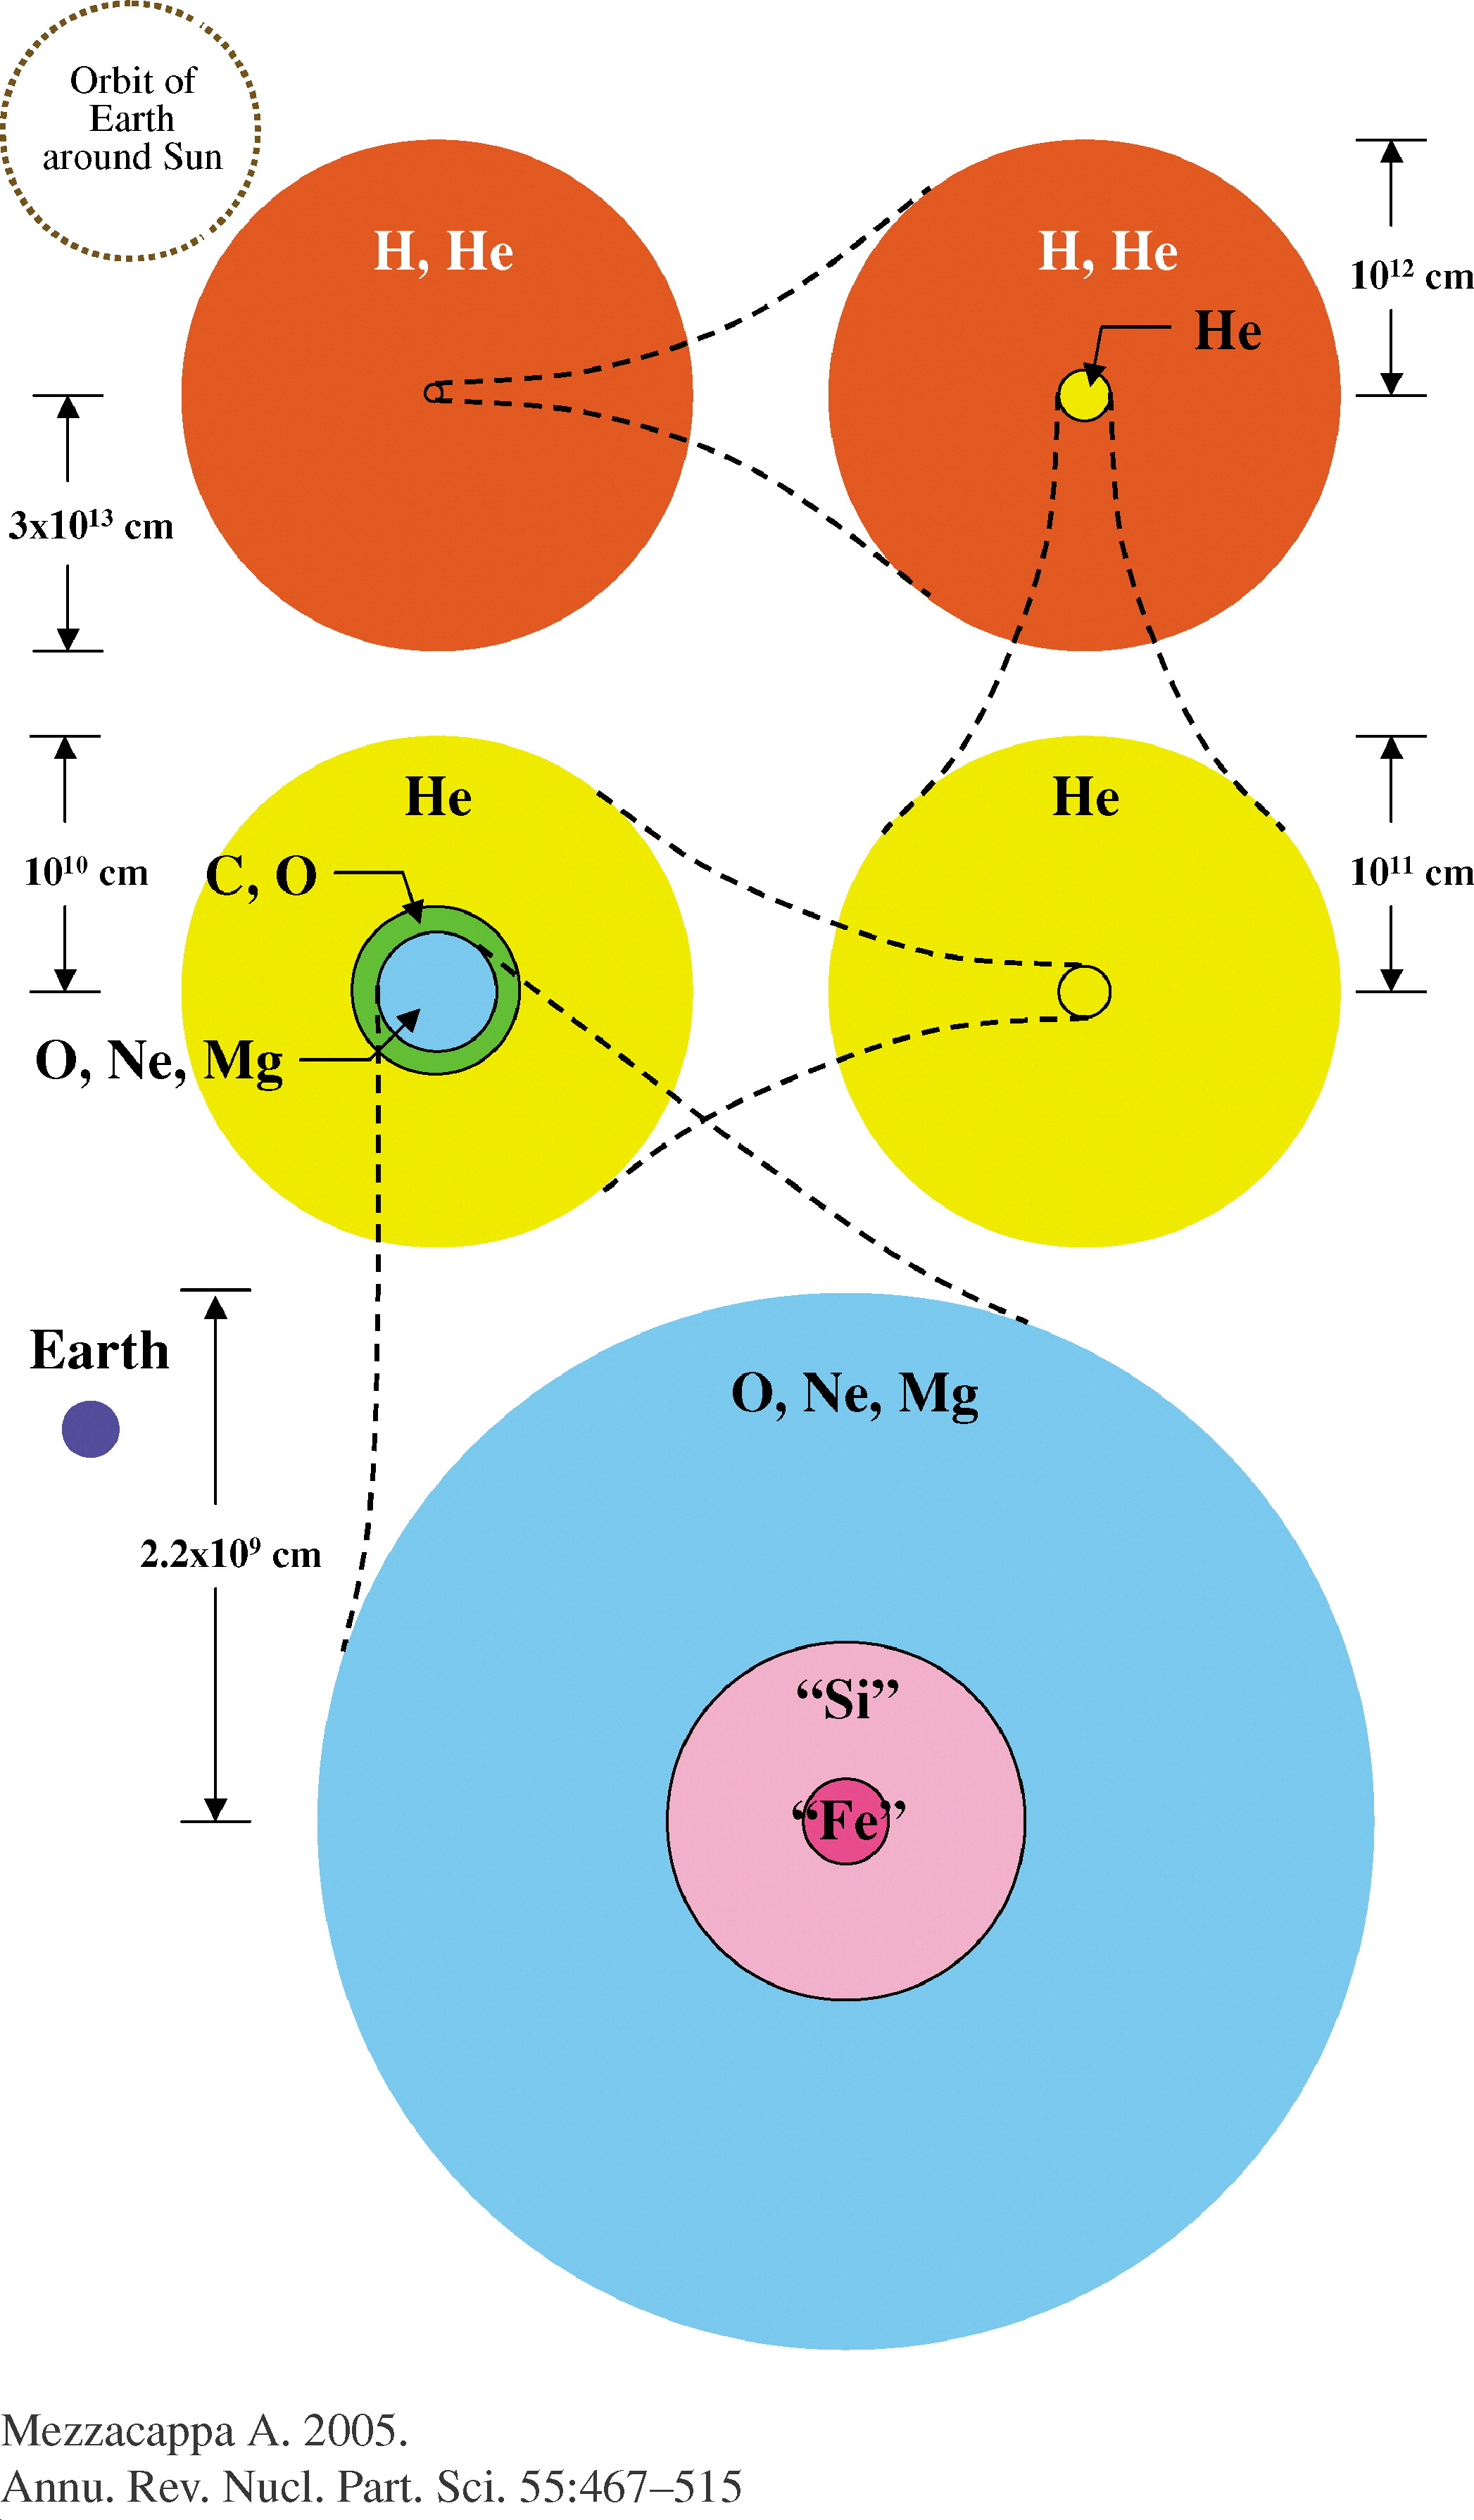
\includegraphics[width=0.25\textwidth]{Figures/onion.jpeg}
  \end{figure}
  Figure from [2]

\end{frame}

\begin{frame}

  \begin{figure}
    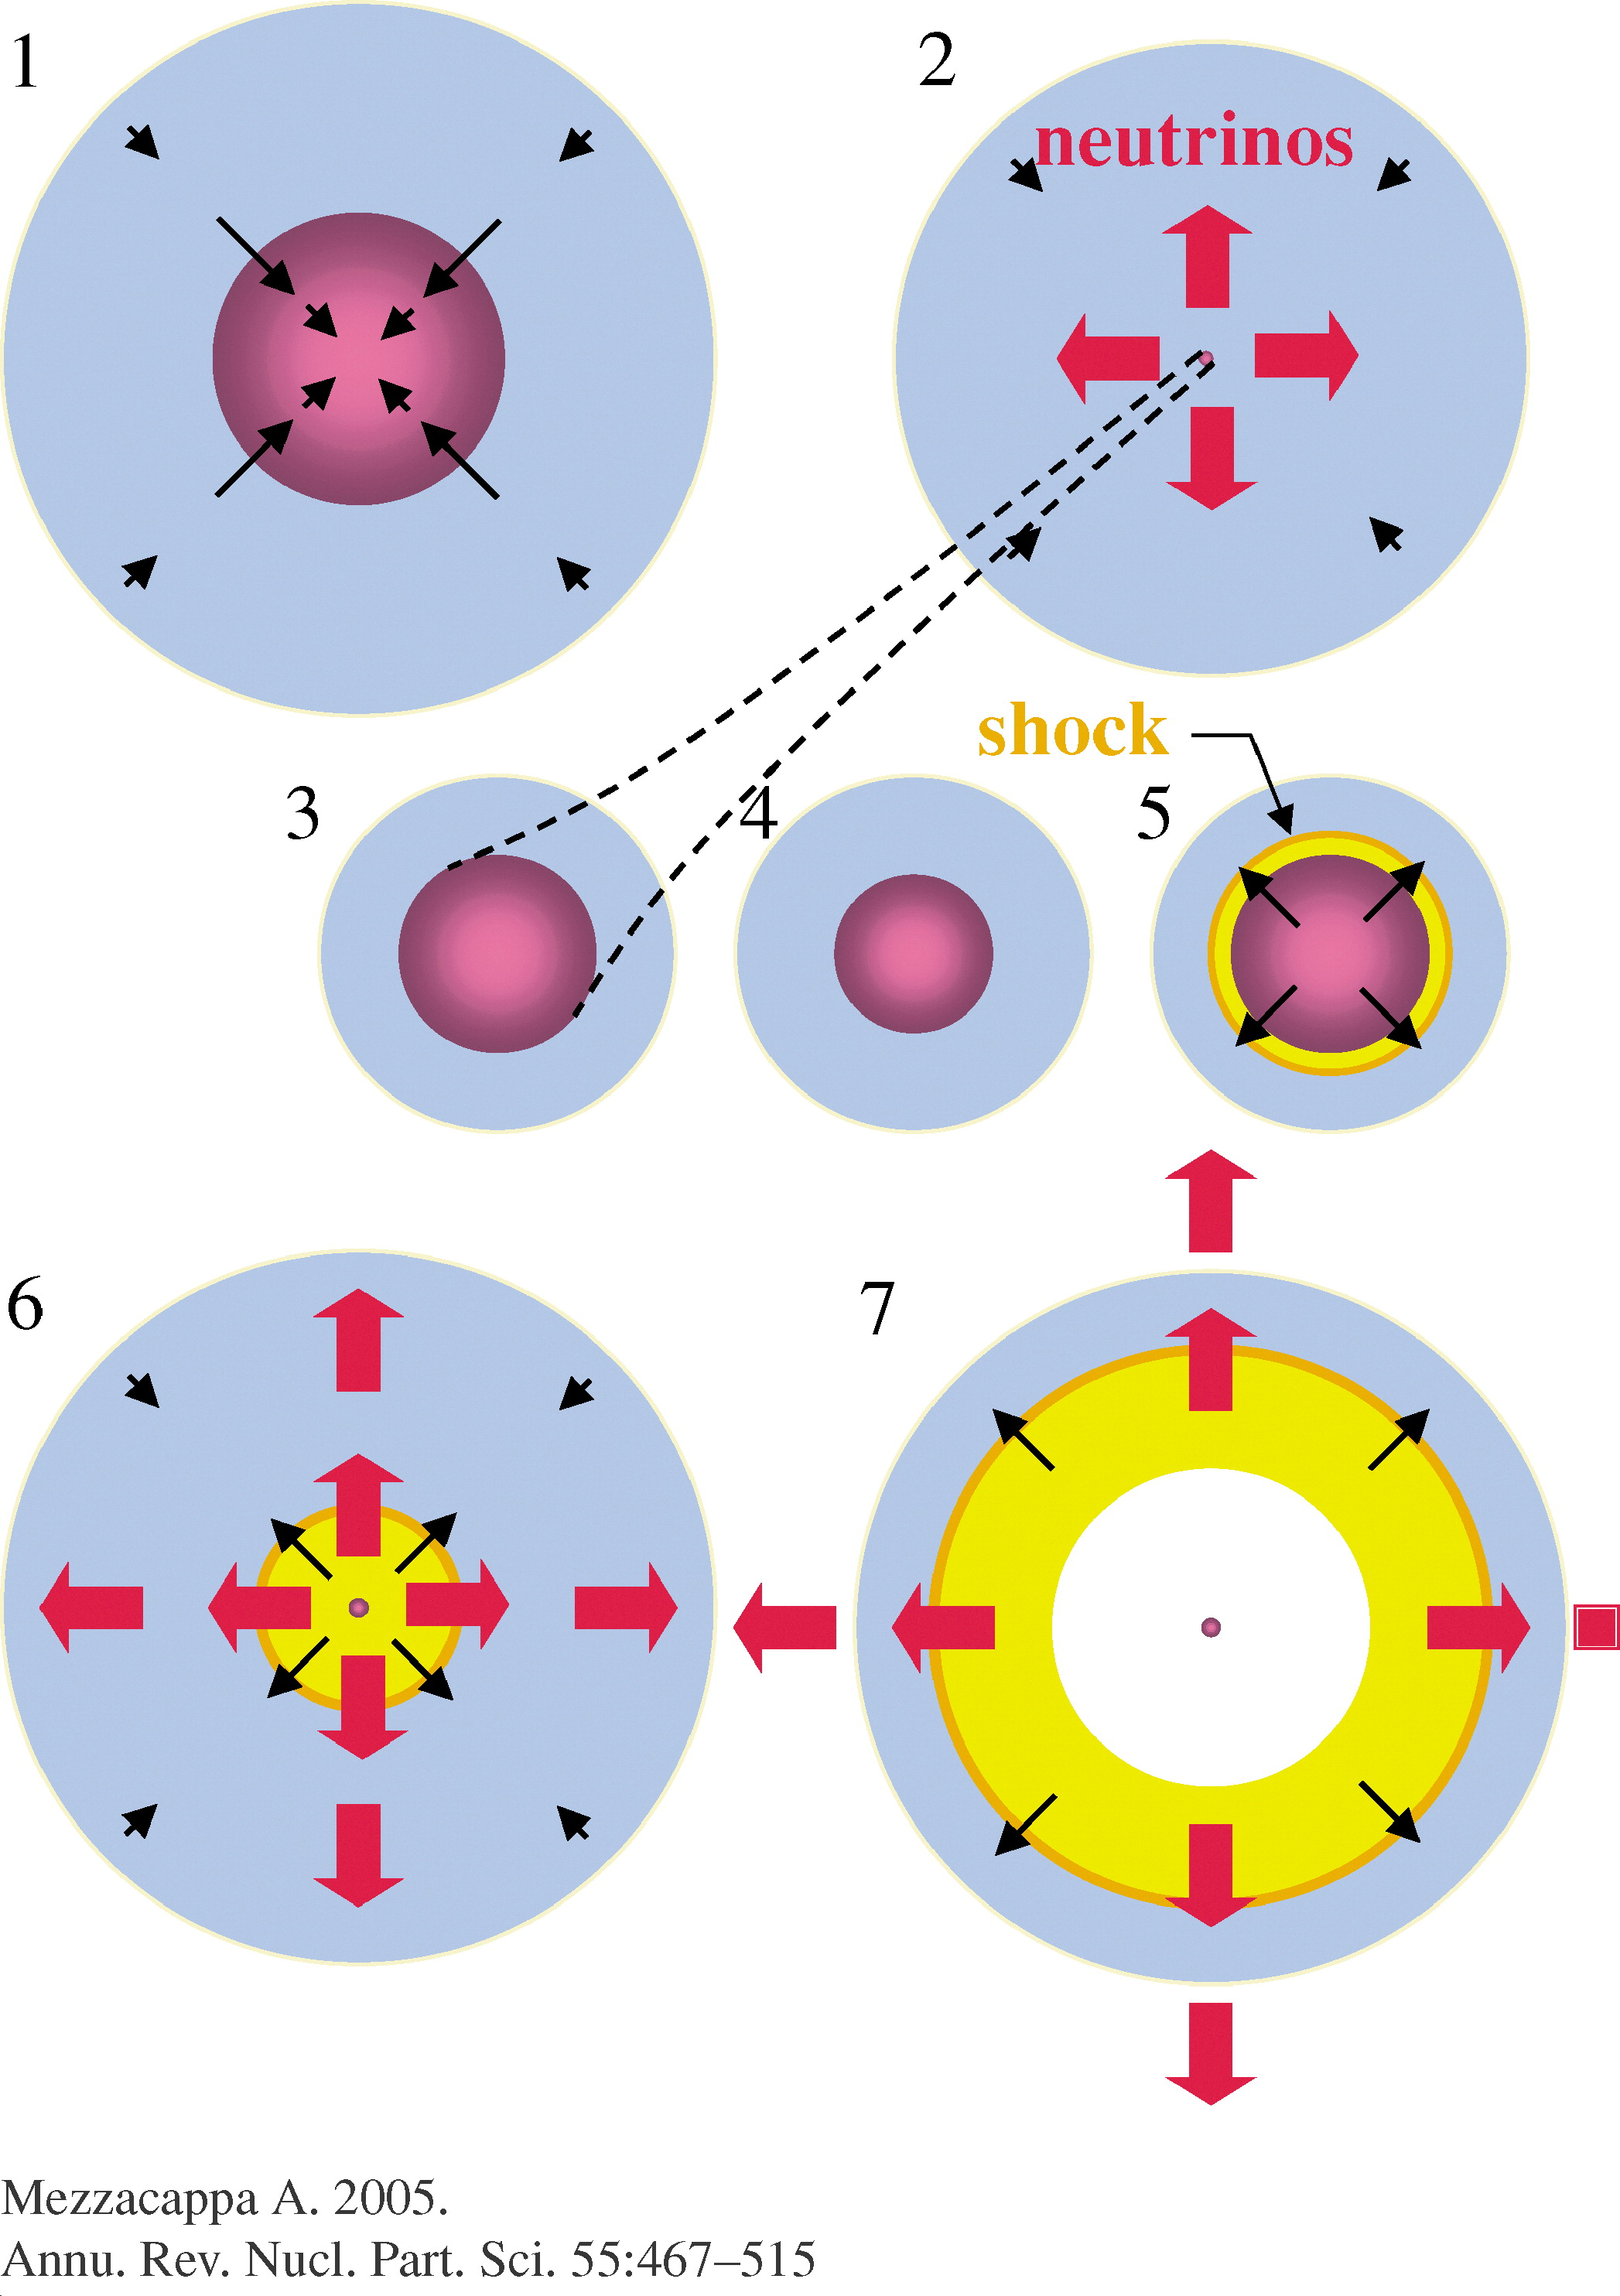
\includegraphics[width=0.3\textwidth]{Figures/explosion.jpeg}
  \end{figure}
  Figure from [2]

\end{frame}

\begin{frame}

  \begin{figure}
    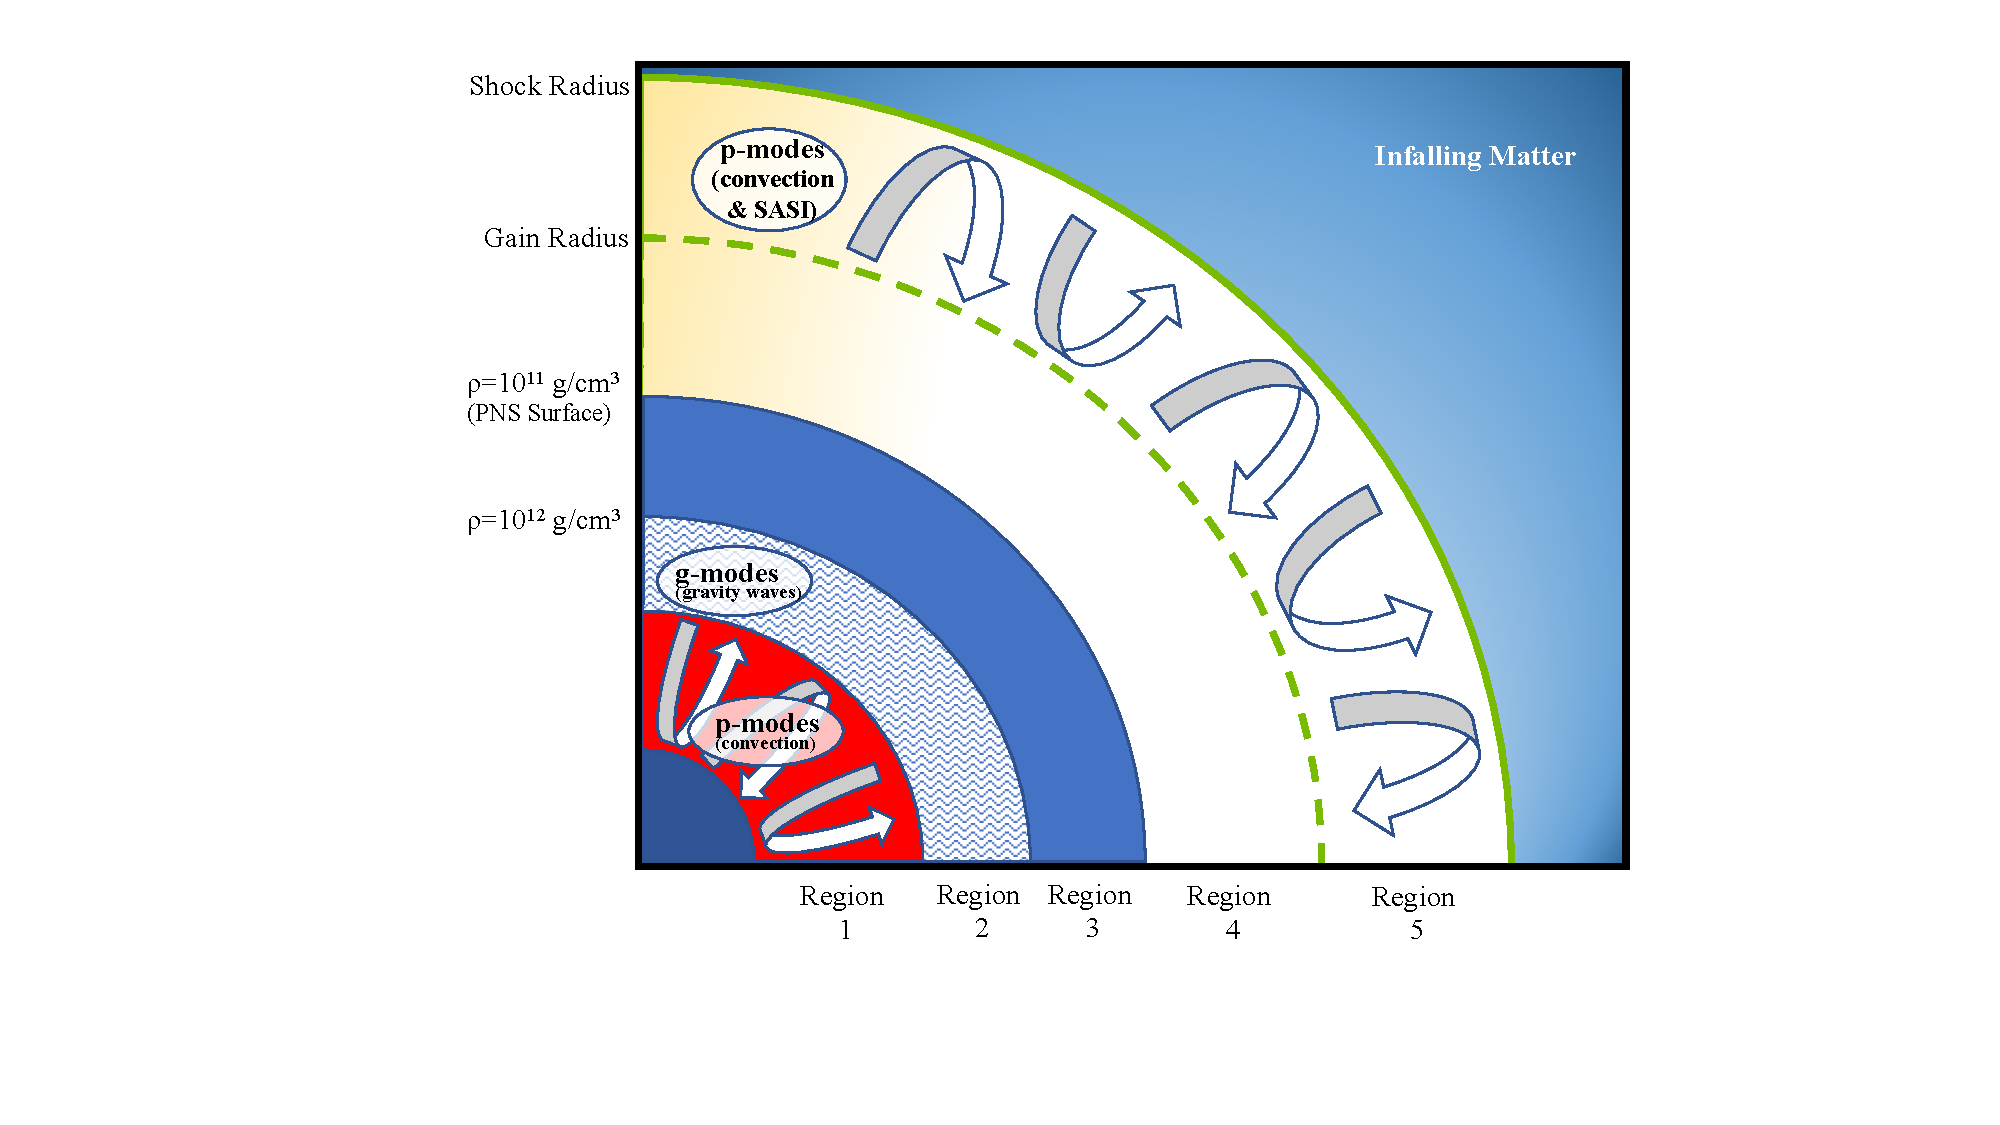
\includegraphics[width=0.6\textwidth]{Figures/regionsCartoon.pdf}
  \end{figure}
  Figure from [3]

\end{frame}

\begin{frame}

  \begin{figure}
    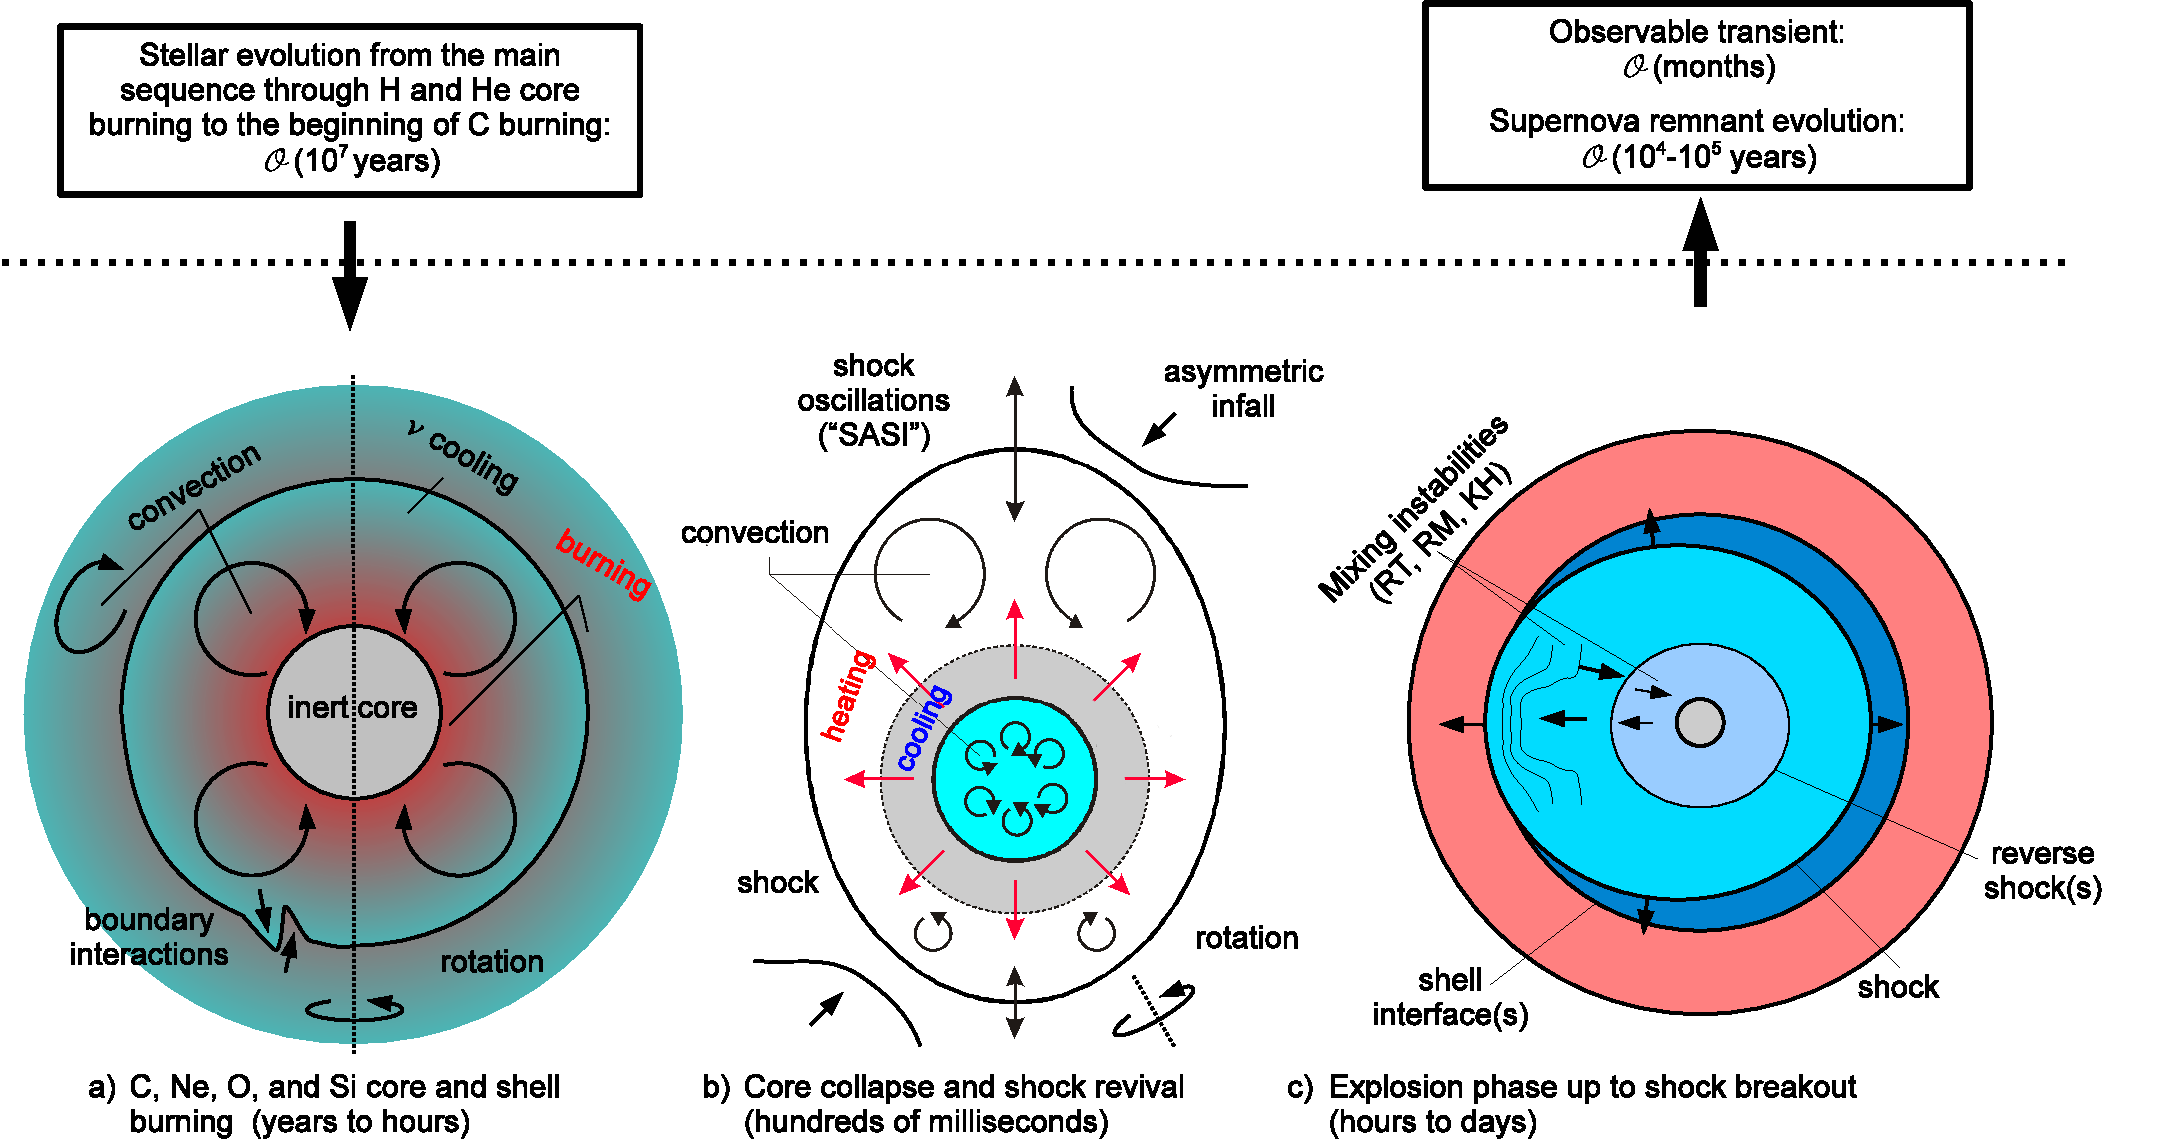
\includegraphics[width=0.8\textwidth]{Figures/asymmetry.pdf}
  \end{figure}
  Figure from [4]

\end{frame}

%-------------------------------------------------------------------------------
\section{Methods}
%-------------------------------------------------------------------------------

\subsection{What They Did}

\begin{frame}

  \textbf{Computed GW-related quantities from three 3D runs with}
  \chimera{}
  \begin{itemize}
    \item Decomposed radial domain into five regions
    \item Computed:
    \begin{itemize}
      \item Strains (``+" and ``$\times$" polarizations)
      \item Spectrograms
      \item Peak frequency evolutions
      \item Luminosities and total energies
      \item Spectra
    \end{itemize}
    \item All Earth-based measurements assume SN distance of $10\,\kpc$
  \end{itemize}

\end{frame}

\begin{frame}

  \begin{columns}[c]

    \column{.5\textwidth} % Left column and width
      \begin{itemize}
        \item MGFLD, RbR+
        \item Newtonian self-gravity + monopole correction
        \item Newtonian hydrodynamics
        \item Yin-Yang grid with $\sim1^{\circ}$
              resolution in $\theta$ and $\varphi$ (Figure from [4])
      \end{itemize}

    \column{.5\textwidth} % Right column and width
      \begin{figure}
        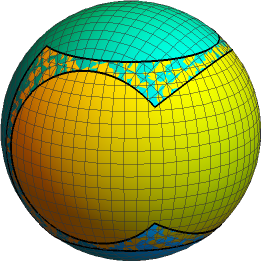
\includegraphics[width=0.8\textwidth]{Figures/yinyang.png}
      \end{figure}

  \end{columns}

\end{frame}

\begin{frame}

  \begin{itemize}
    \item Three masses:
          $M/\msun\in\left\{9.6,15,25\right\}$
    \item D9.6 and D25 had zero metallicity
    \item D15 had Solar metallicity
    \item No rotation
    \item No magnetic fields
  \end{itemize}

\end{frame}

\begin{frame}

  \begin{columns}[c]

    \column{.5\textwidth} % Left column and width
      \begin{figure}
        \textbf{D15}
        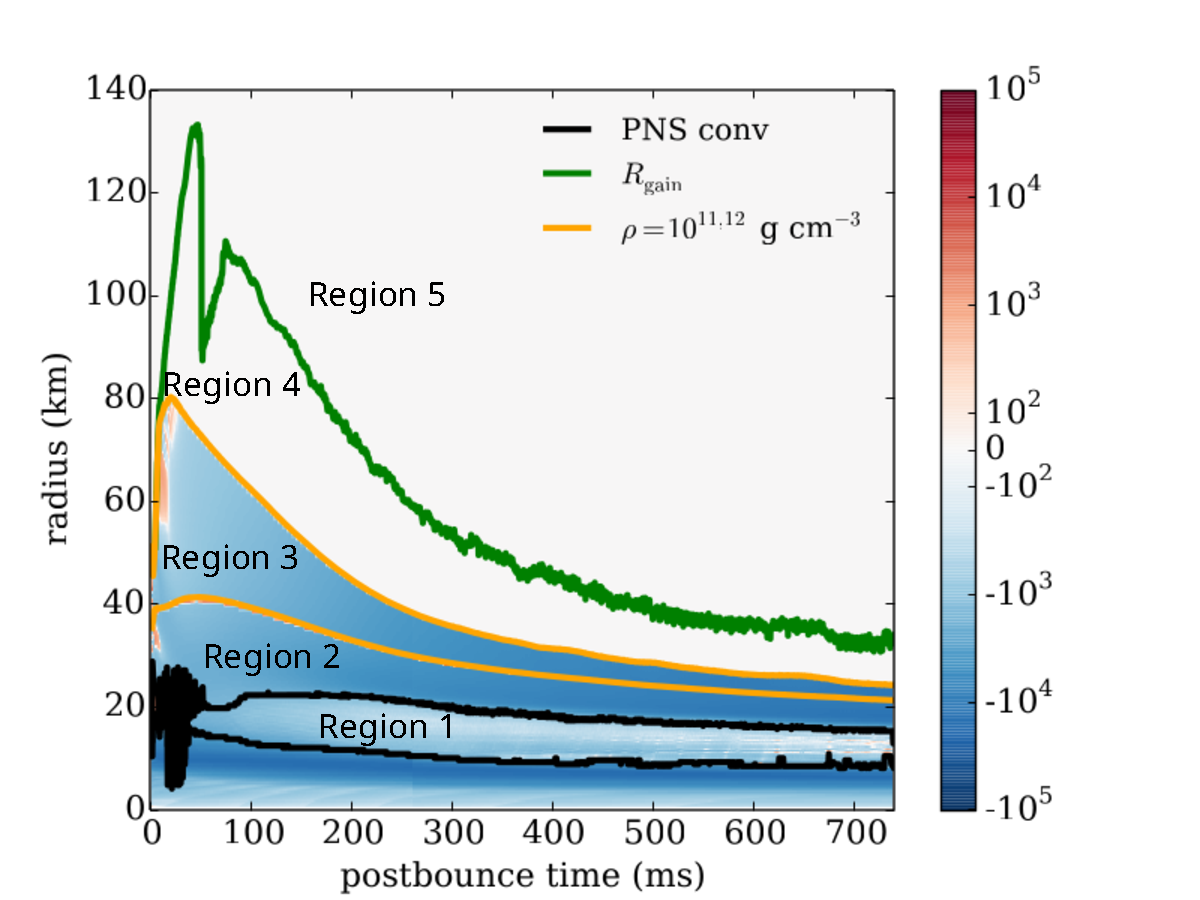
\includegraphics[width=1.1\textwidth]{Figures/D15_regions.pdf}
      \end{figure}

    \column{.5\textwidth} % Right column and width
      \begin{figure}
        \textbf{D25}
        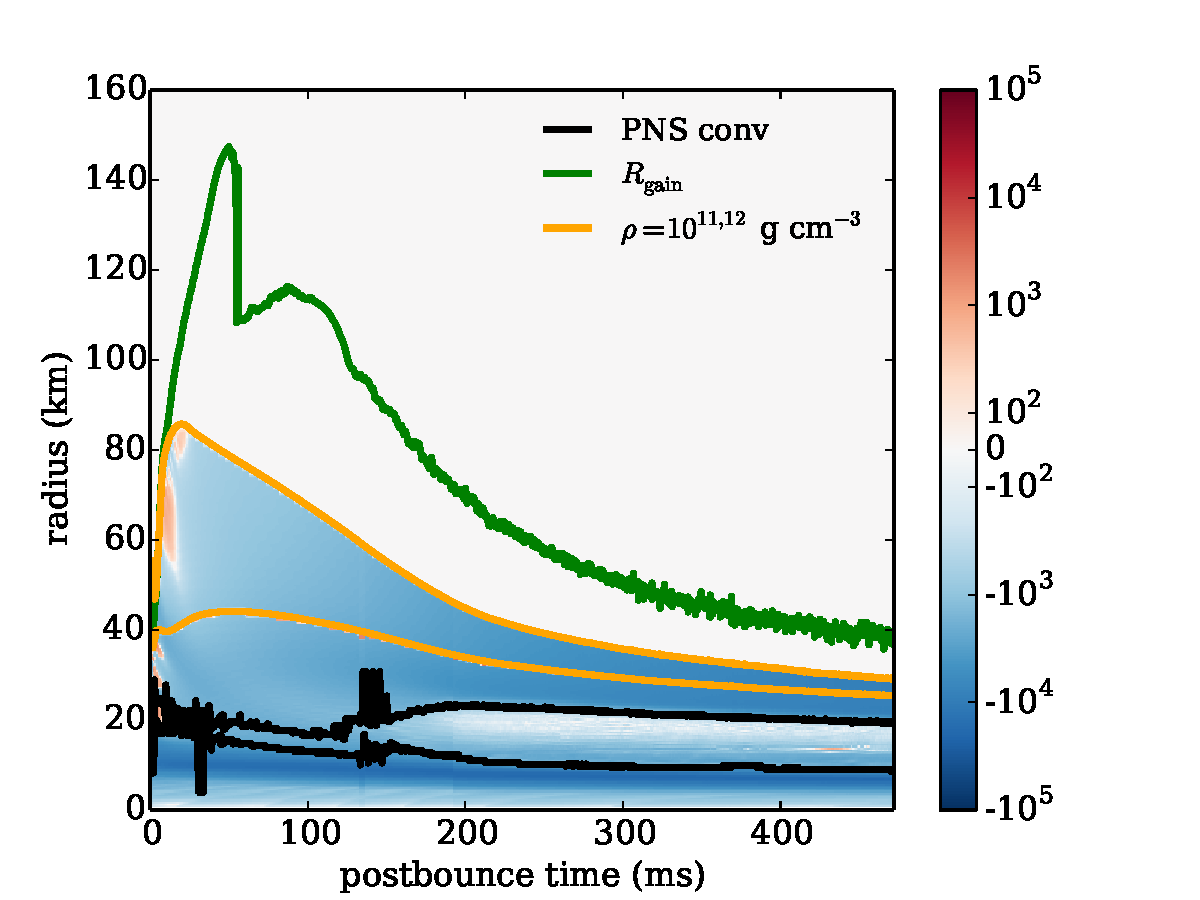
\includegraphics[width=1.1\textwidth]{Figures/D25_regions.pdf}
      \end{figure}

  \end{columns}

\end{frame}

\begin{frame}

  \hspace{16em}\textbf{D9.6}
  \vspace{-0.5em}
  \begin{figure}
    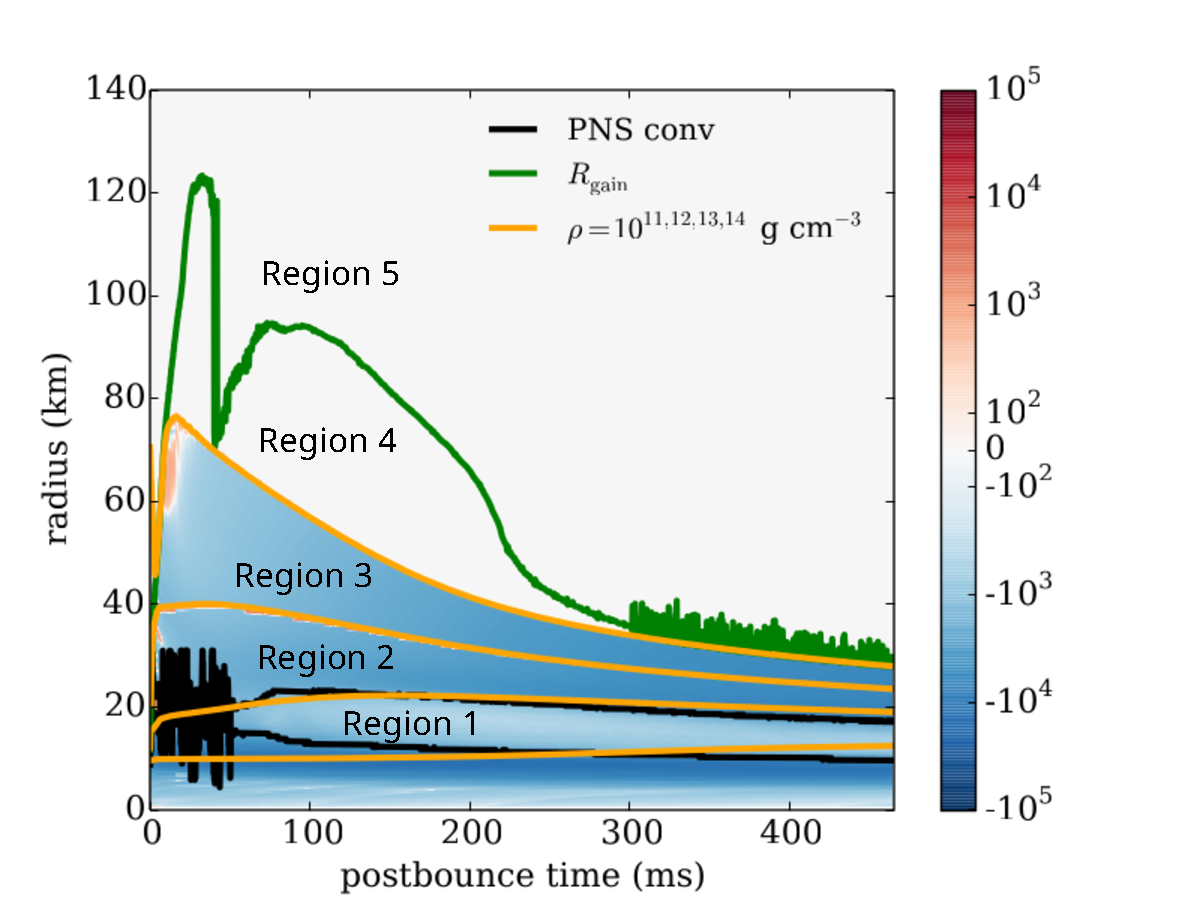
\includegraphics[width=0.6\textwidth]{Figures/D9.6_regions.pdf}
  \end{figure}

\end{frame}

%-------------------------------------------------------------------------------
\section{Results}
%-------------------------------------------------------------------------------

\subsection{Strains}

\begin{frame}

  \hspace{8em}\textbf{D9.6}\hspace{7em}\textbf{D15}\hspace{7em}\textbf{D25}
  \vspace{-1.5em}
  \begin{figure}
    \centering
    \subfloat{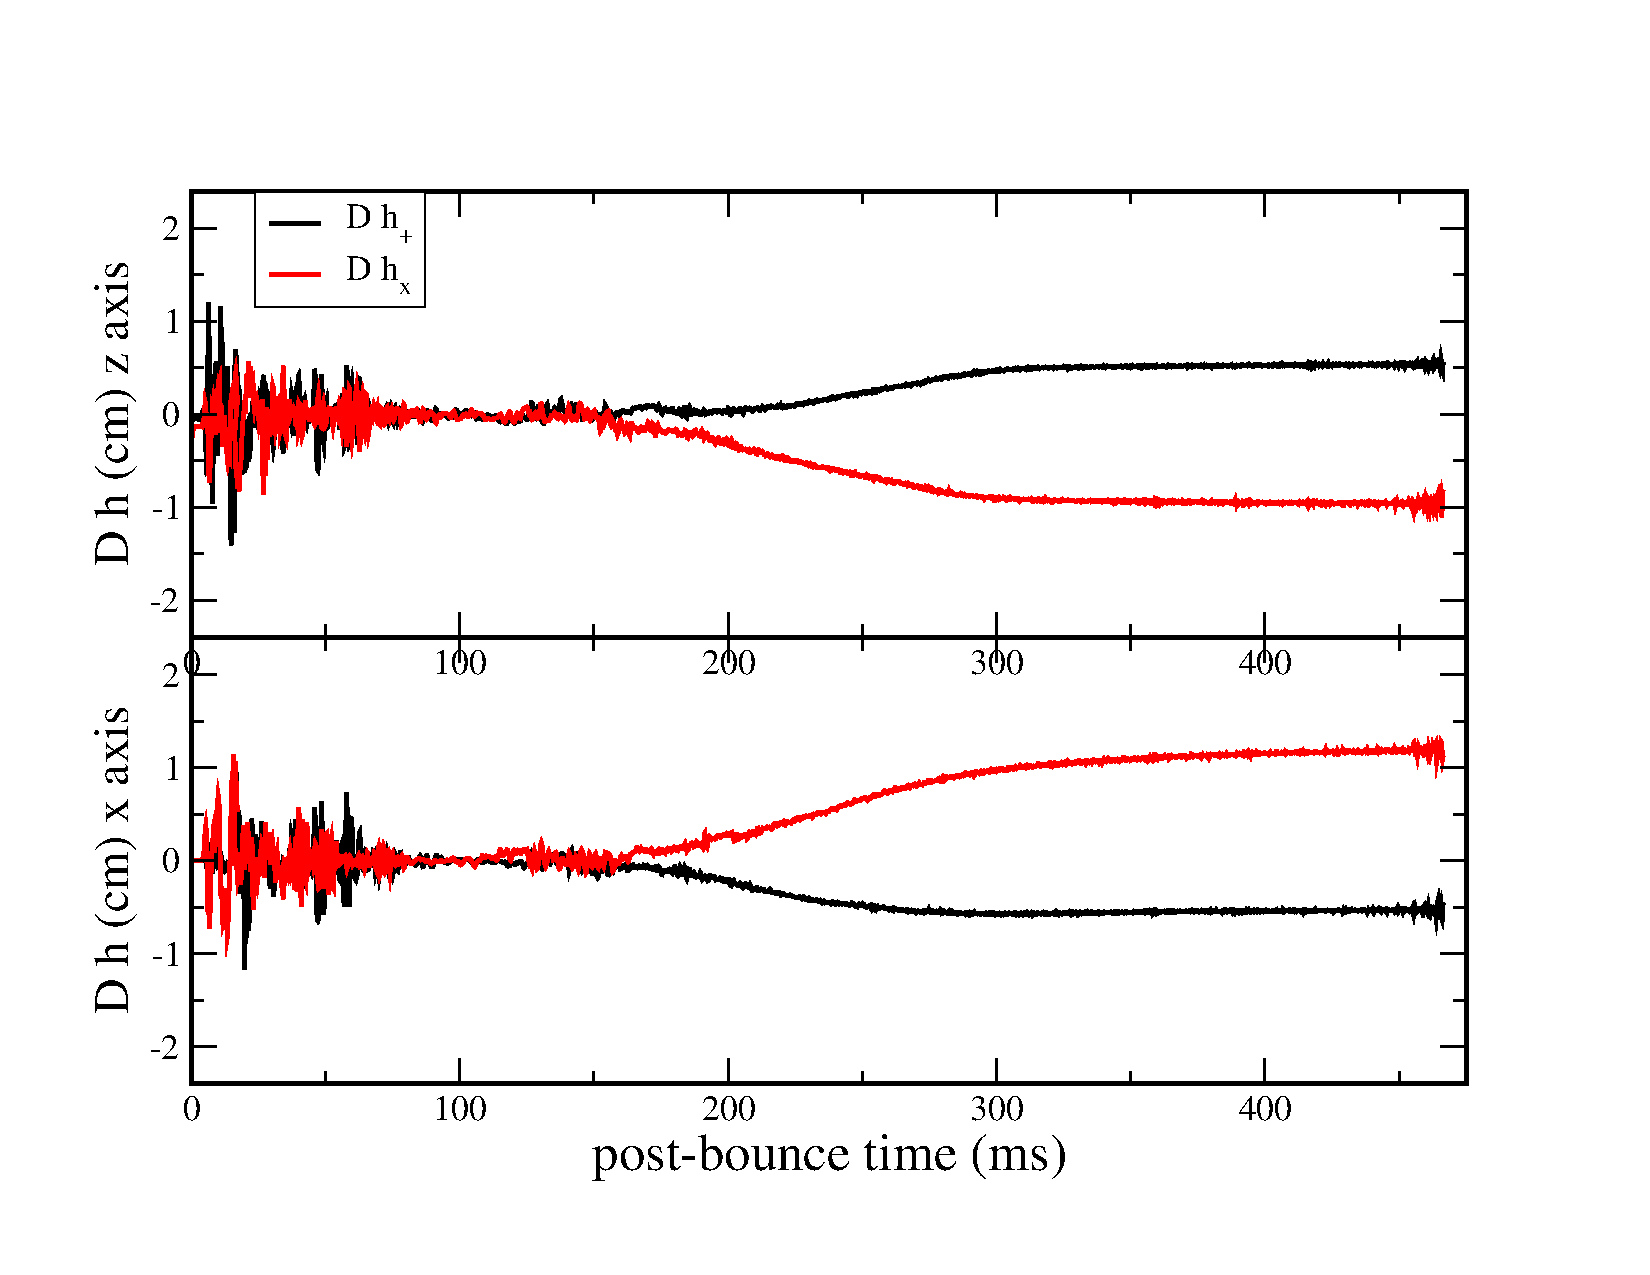
\includegraphics[width=0.25\textwidth]{Figures/D9.6_strain.pdf}}
    \subfloat{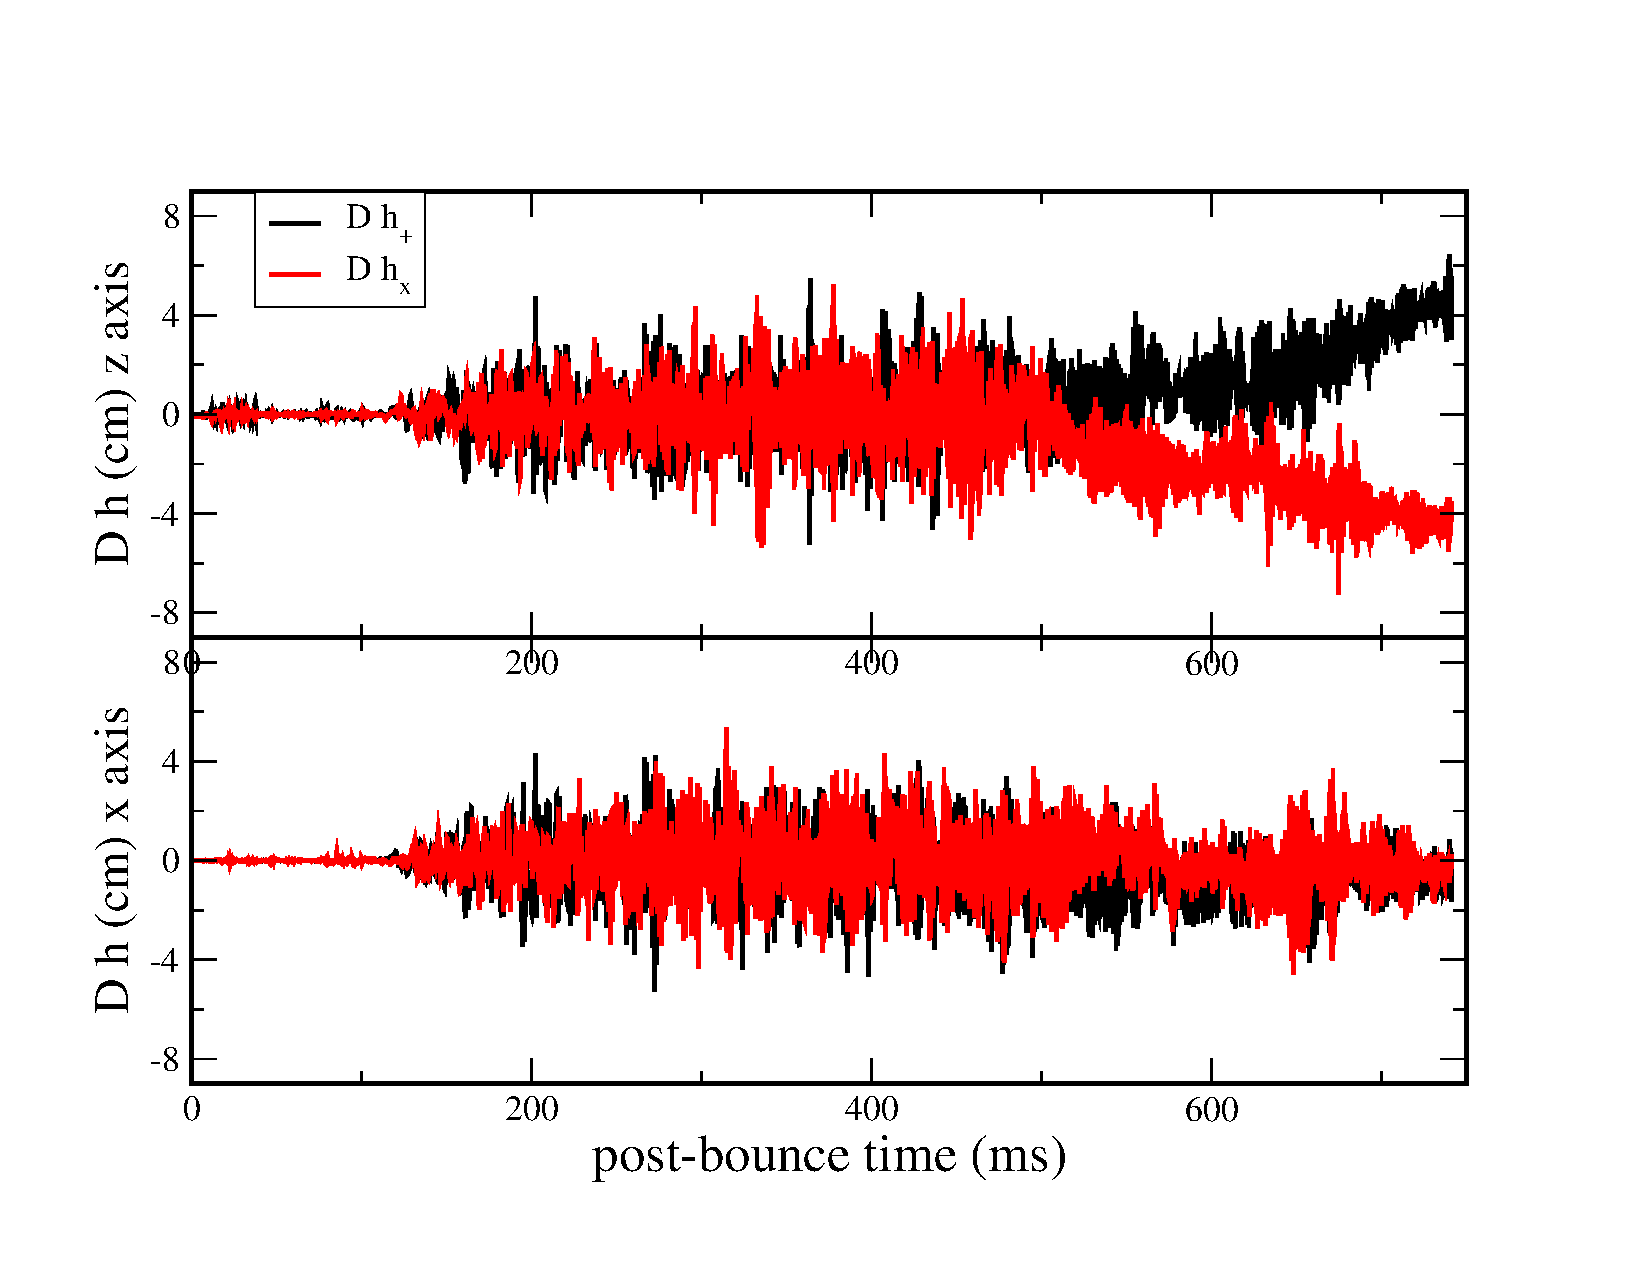
\includegraphics[width=0.25\textwidth]{Figures/D15_strain.pdf}}
    \subfloat{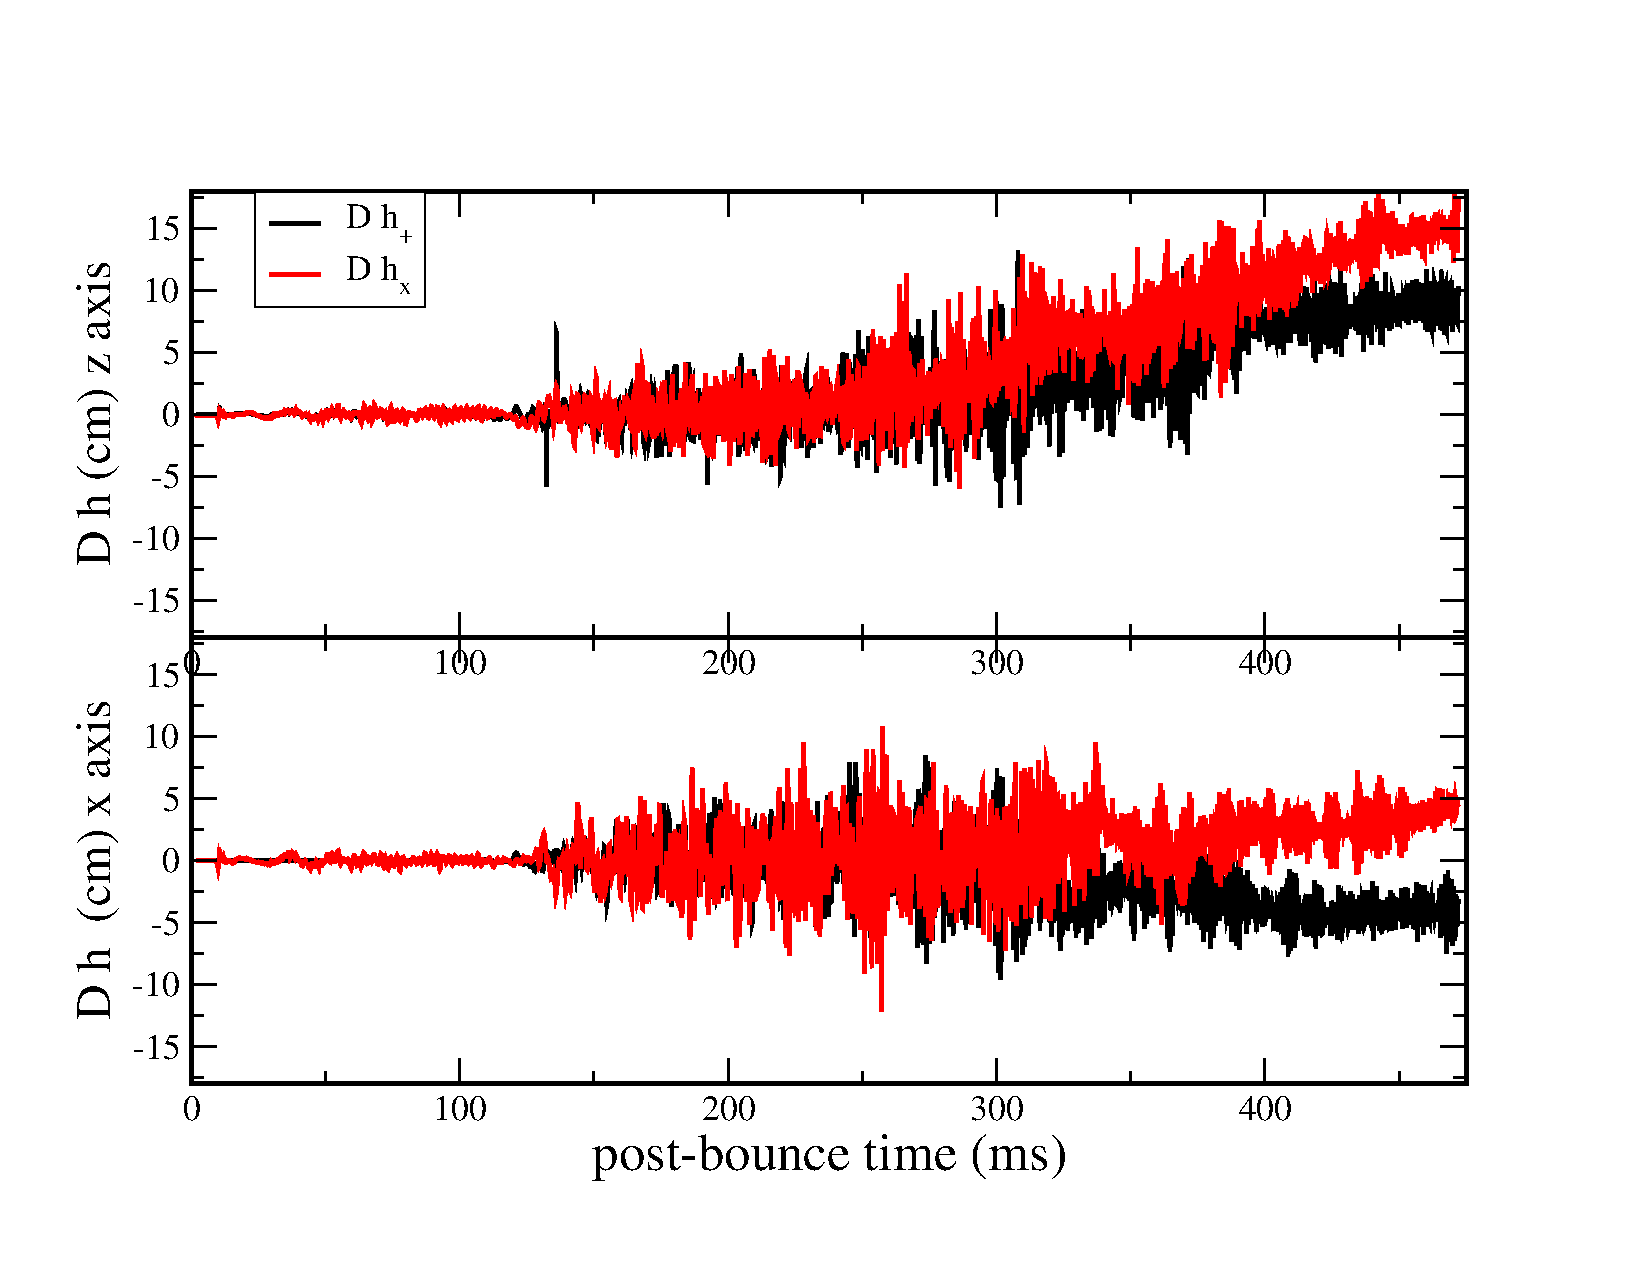
\includegraphics[width=0.25\textwidth]{Figures/D25_strain.pdf}}
  \end{figure}
  \vspace{-2em}
  \begin{figure}
    \centering
    \subfloat{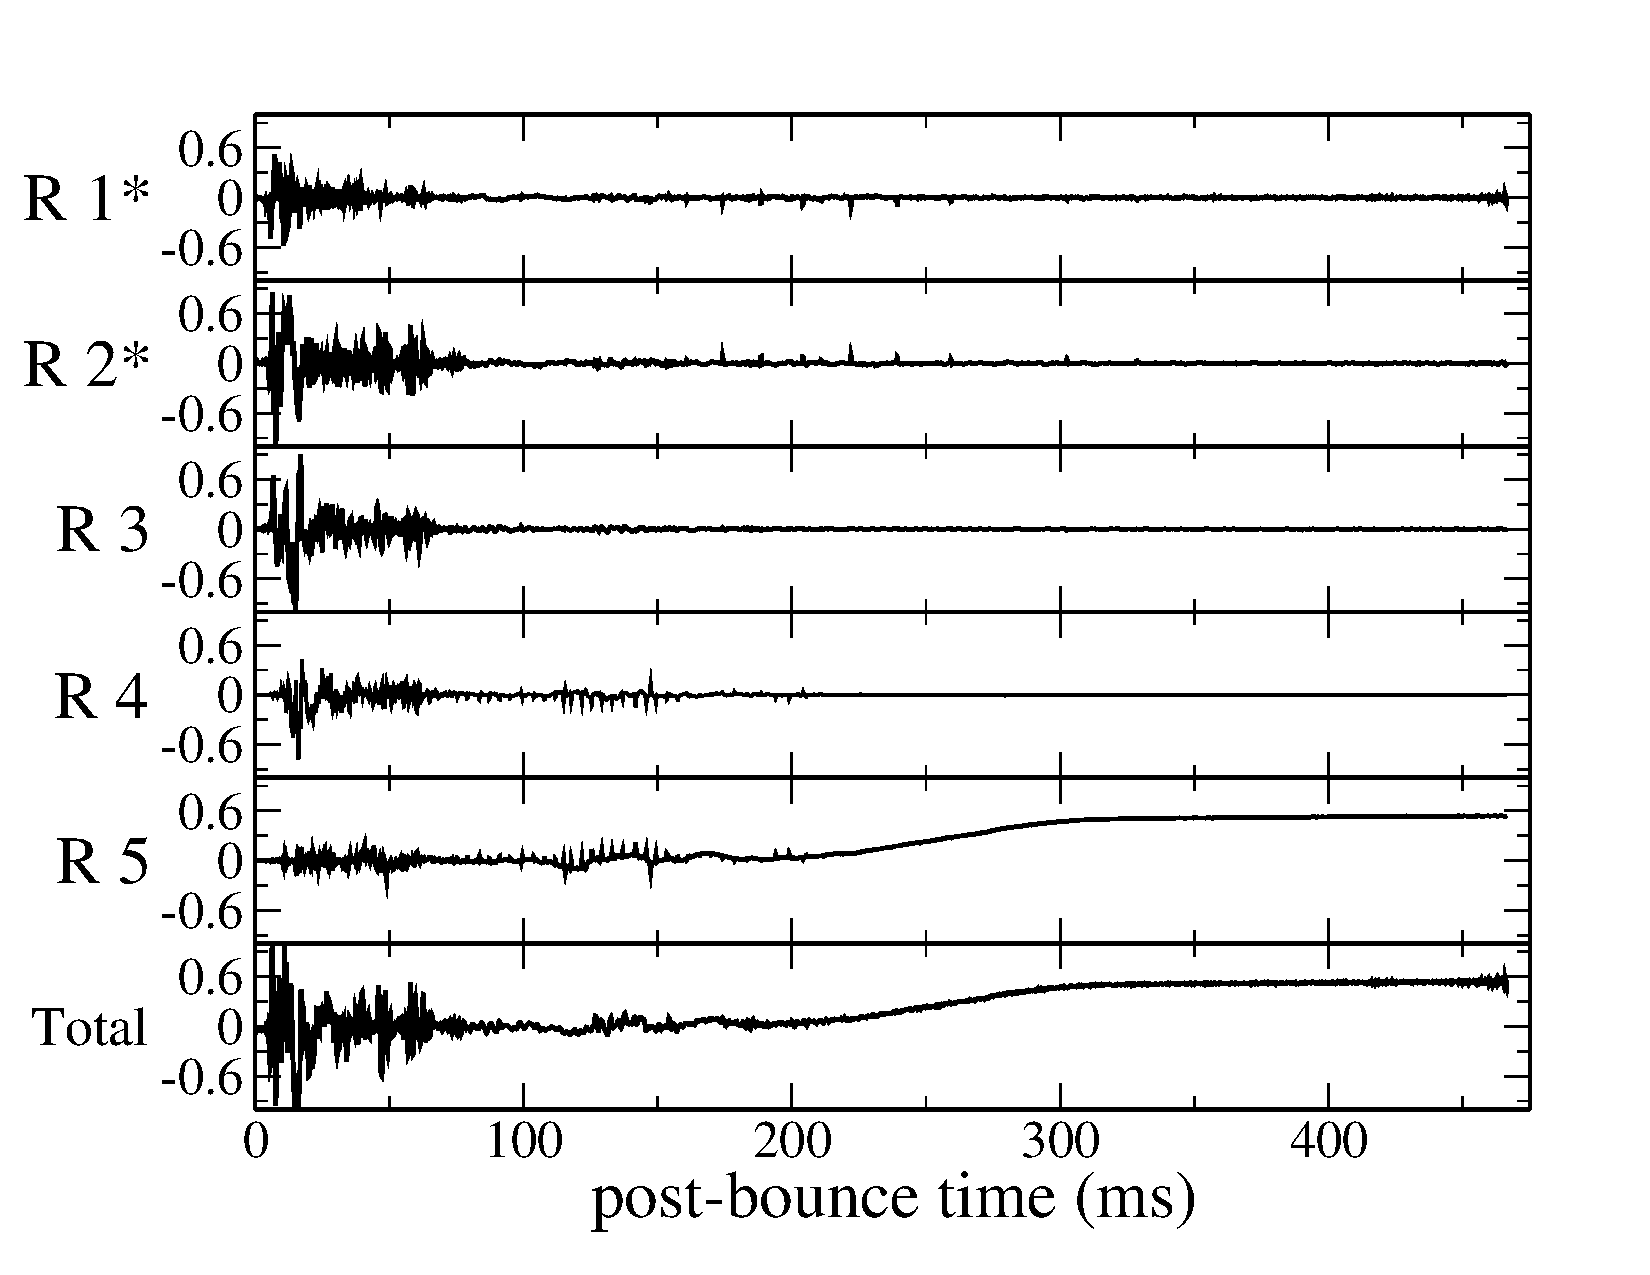
\includegraphics[width=0.25\textwidth]{Figures/D9.6_strain_byRegions_all.pdf}}
    \subfloat{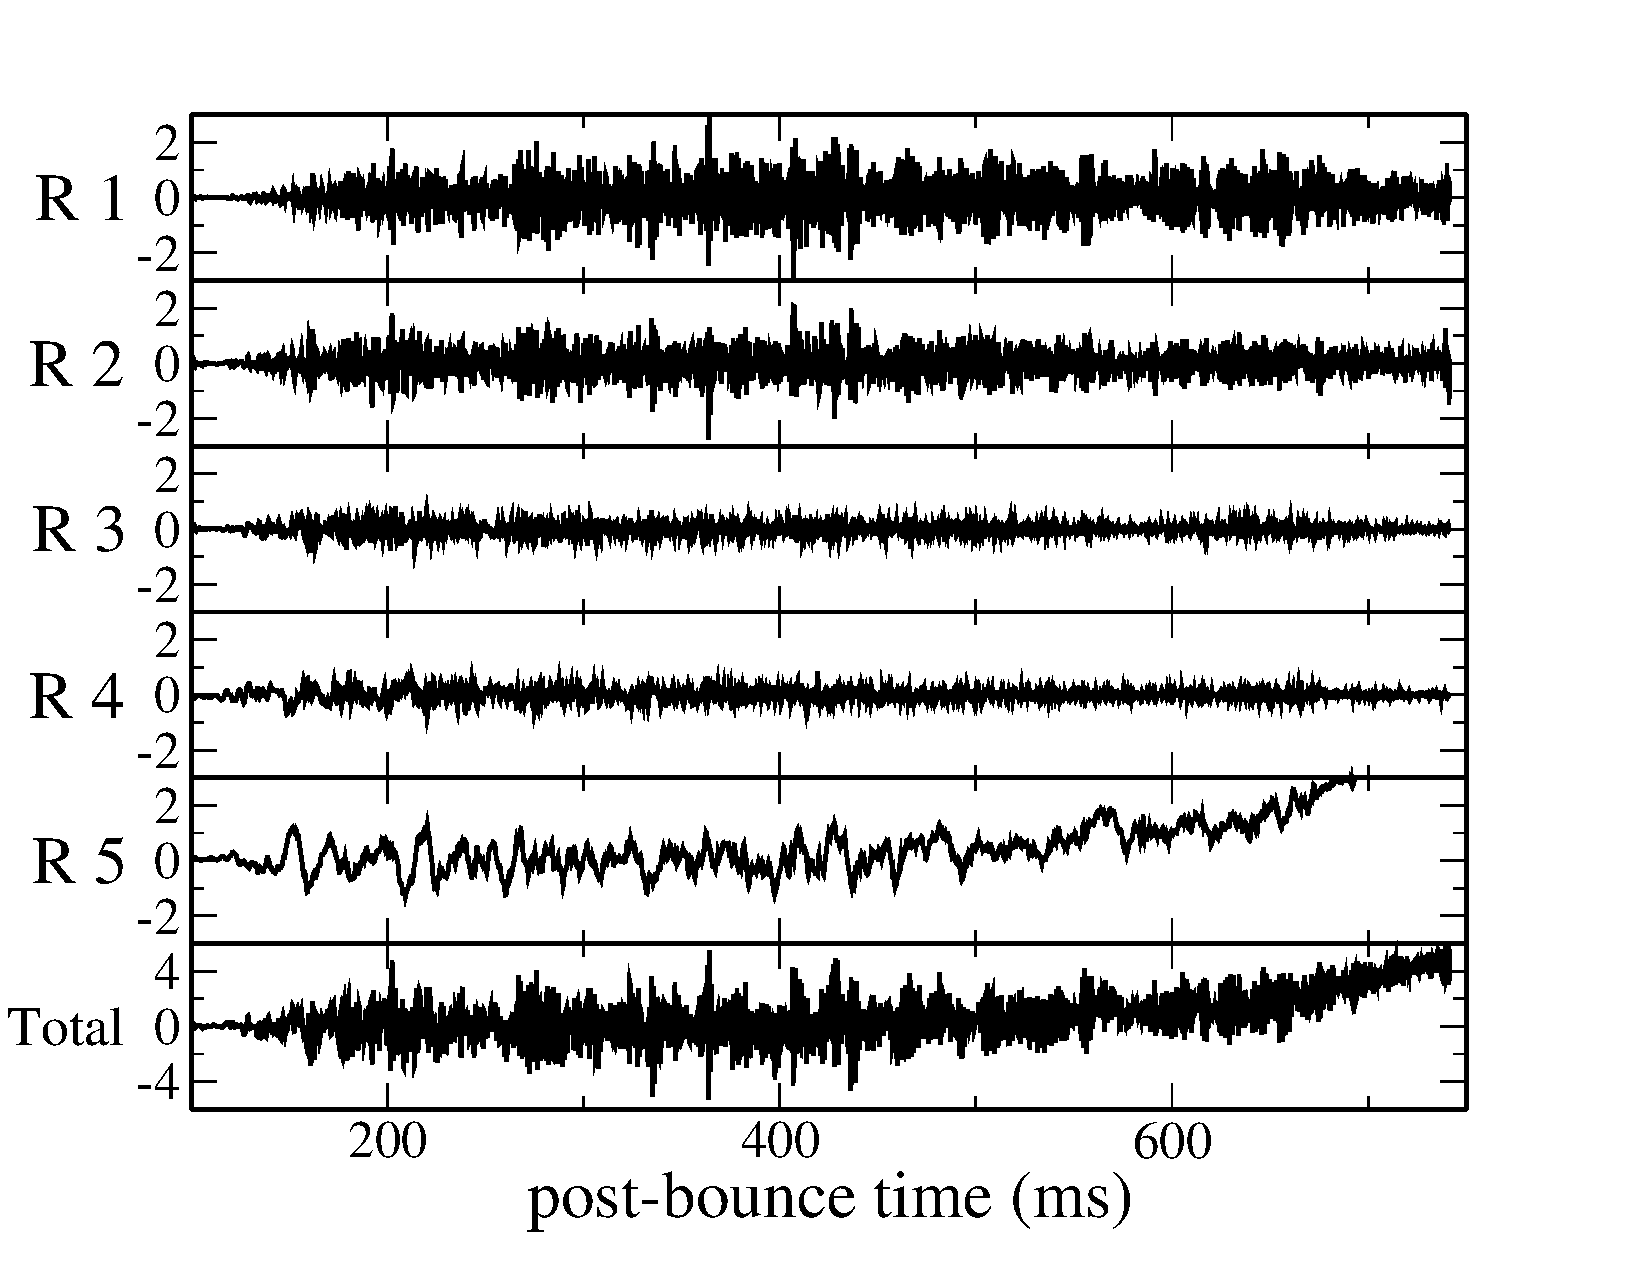
\includegraphics[width=0.25\textwidth]{Figures/D15_strain_byRegions.pdf}}
    \subfloat{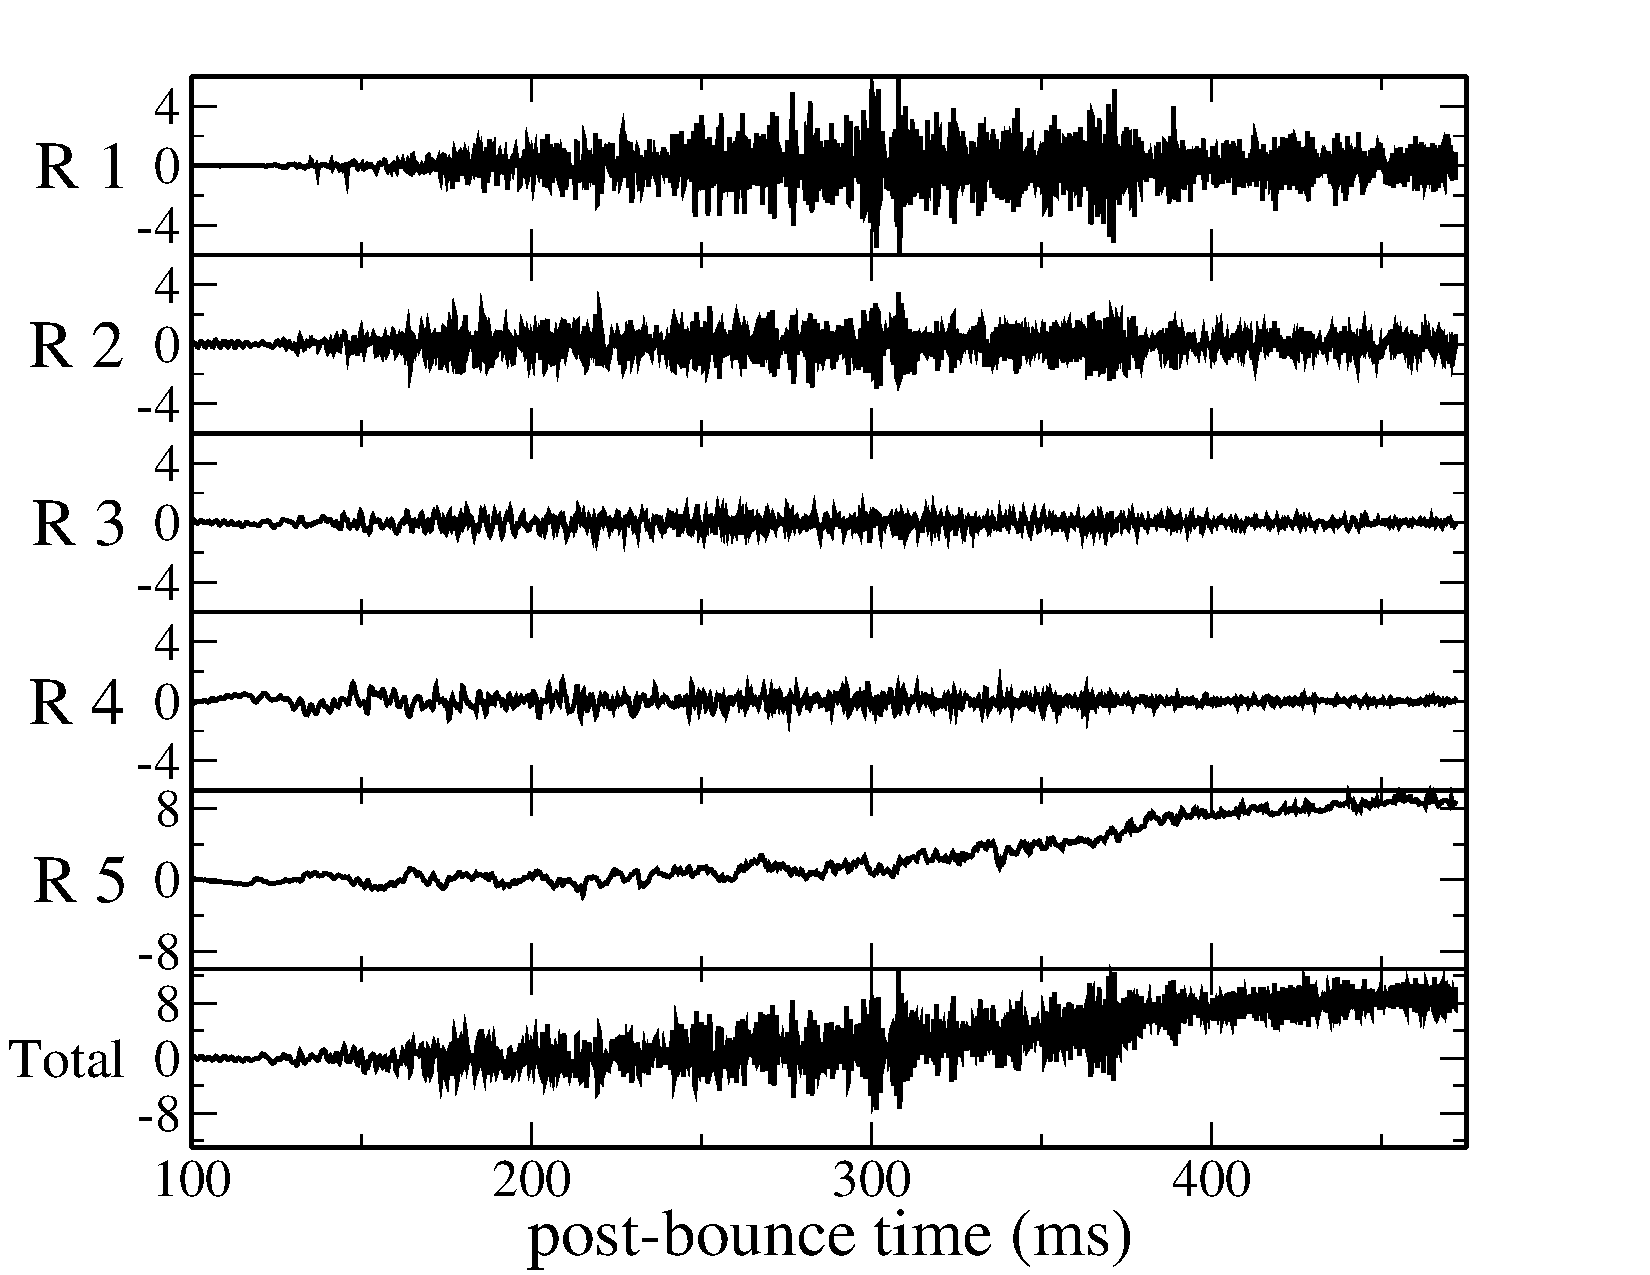
\includegraphics[width=0.25\textwidth]{Figures/D25_strain_byRegions.pdf}}
  \end{figure}

\end{frame}

\begin{frame}

  \centerline{\textbf{D9.6}}
  \vspace{-2em}

  \begin{columns}[c]

    \column{.5\textwidth} % Left column and width
      \begin{figure}
        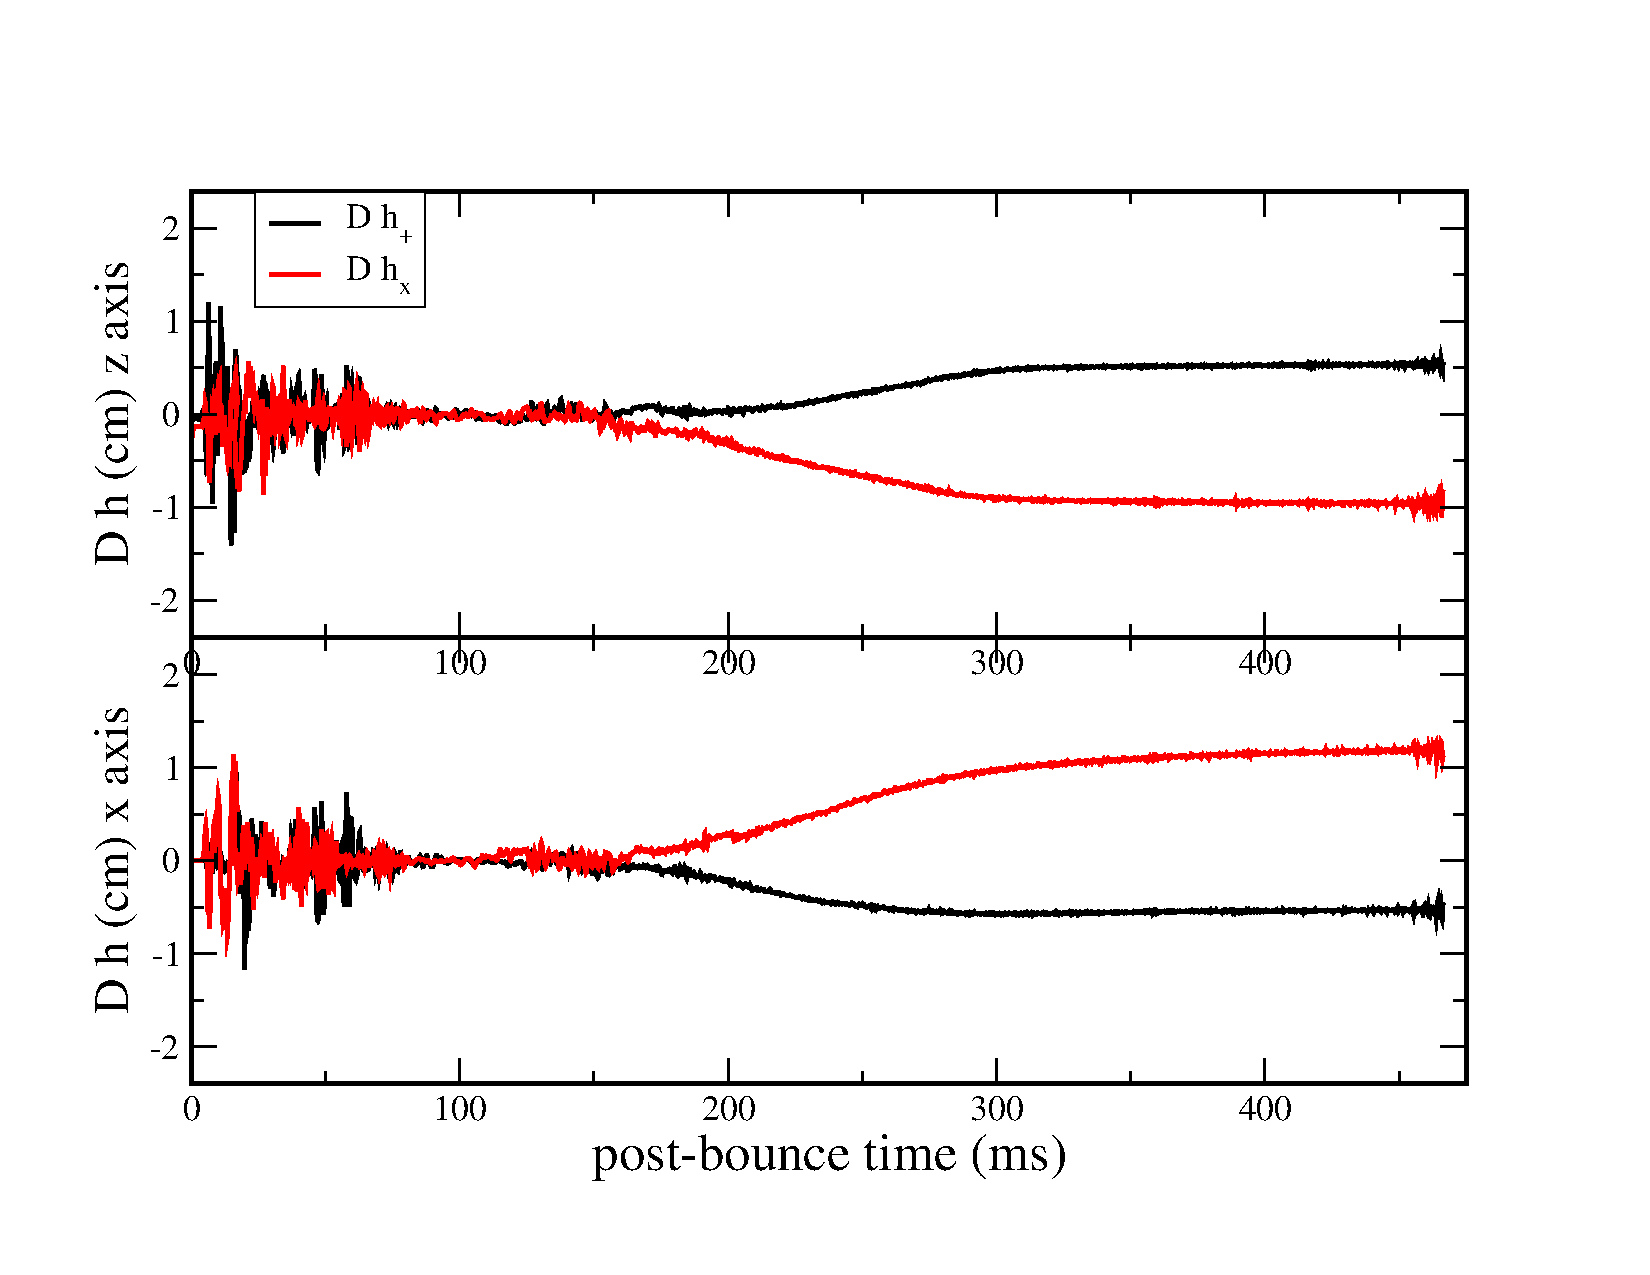
\includegraphics[width=1.1\textwidth]{Figures/D9.6_strain.pdf}
      \end{figure}

    \column{.5\textwidth} % Right column and width
      \begin{figure}
        \includegraphics[width=1.1\textwidth]%
        {Figures/D9.6_strain_byRegions_all.pdf}
      \end{figure}

  \end{columns}

\end{frame}

\begin{frame}

  \centerline{\textbf{D9.6}}

  \begin{figure}
    \includegraphics[width=0.6\textwidth]%
    {Figures/D9.6_strain_byRegions.pdf}
  \end{figure}

\end{frame}

\begin{frame}

  \begin{columns}[c]

    \column{.5\textwidth} % Left column and width
      \begin{figure}
        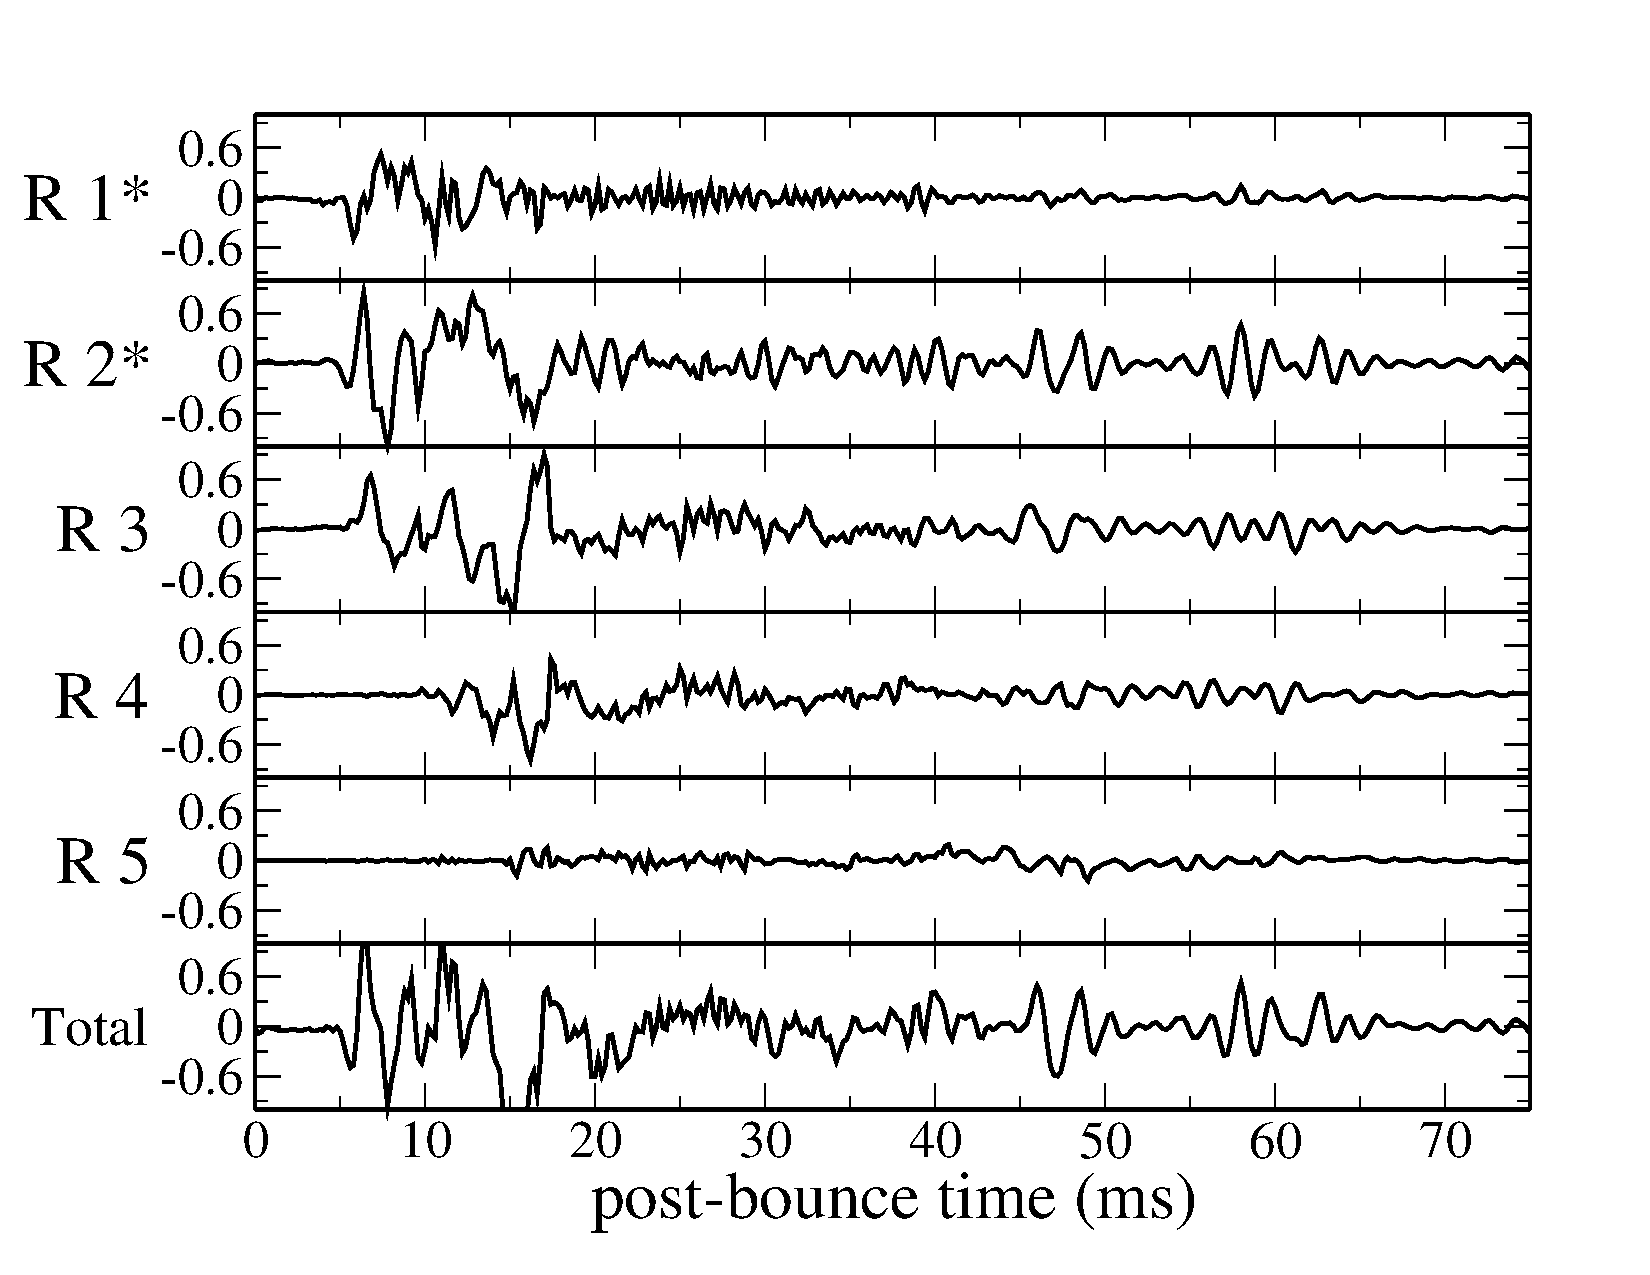
\includegraphics[width=1.0\textwidth]{Figures/D9.6_strain_byRegions.pdf}
      \end{figure}

    \column{.5\textwidth} % Right column and width
      \begin{figure}
        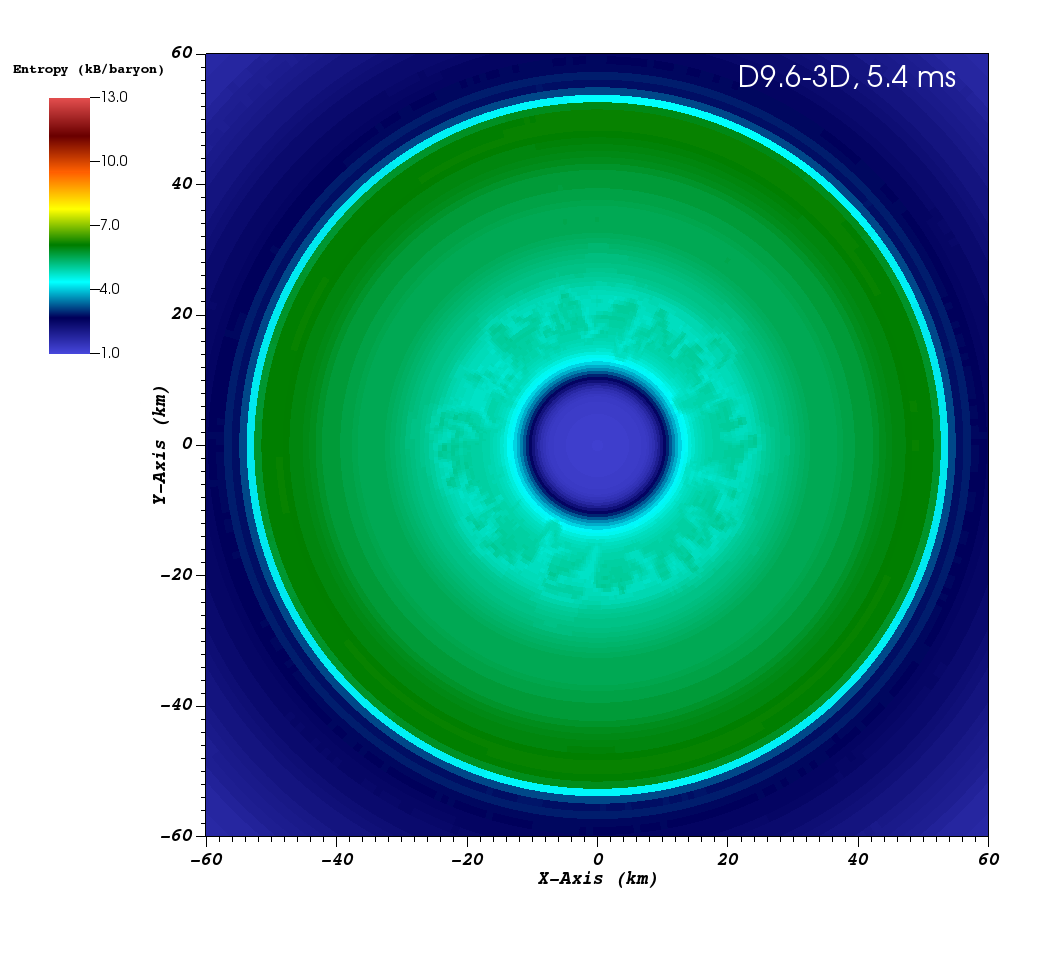
\includegraphics[width=1.0\textwidth]{Figures/D9.6_entropy_5.4ms.png}
      \end{figure}

  \end{columns}

\end{frame}

\begin{frame}

  \begin{columns}[c]

    \column{.5\textwidth} % Left column and width
      \begin{figure}
        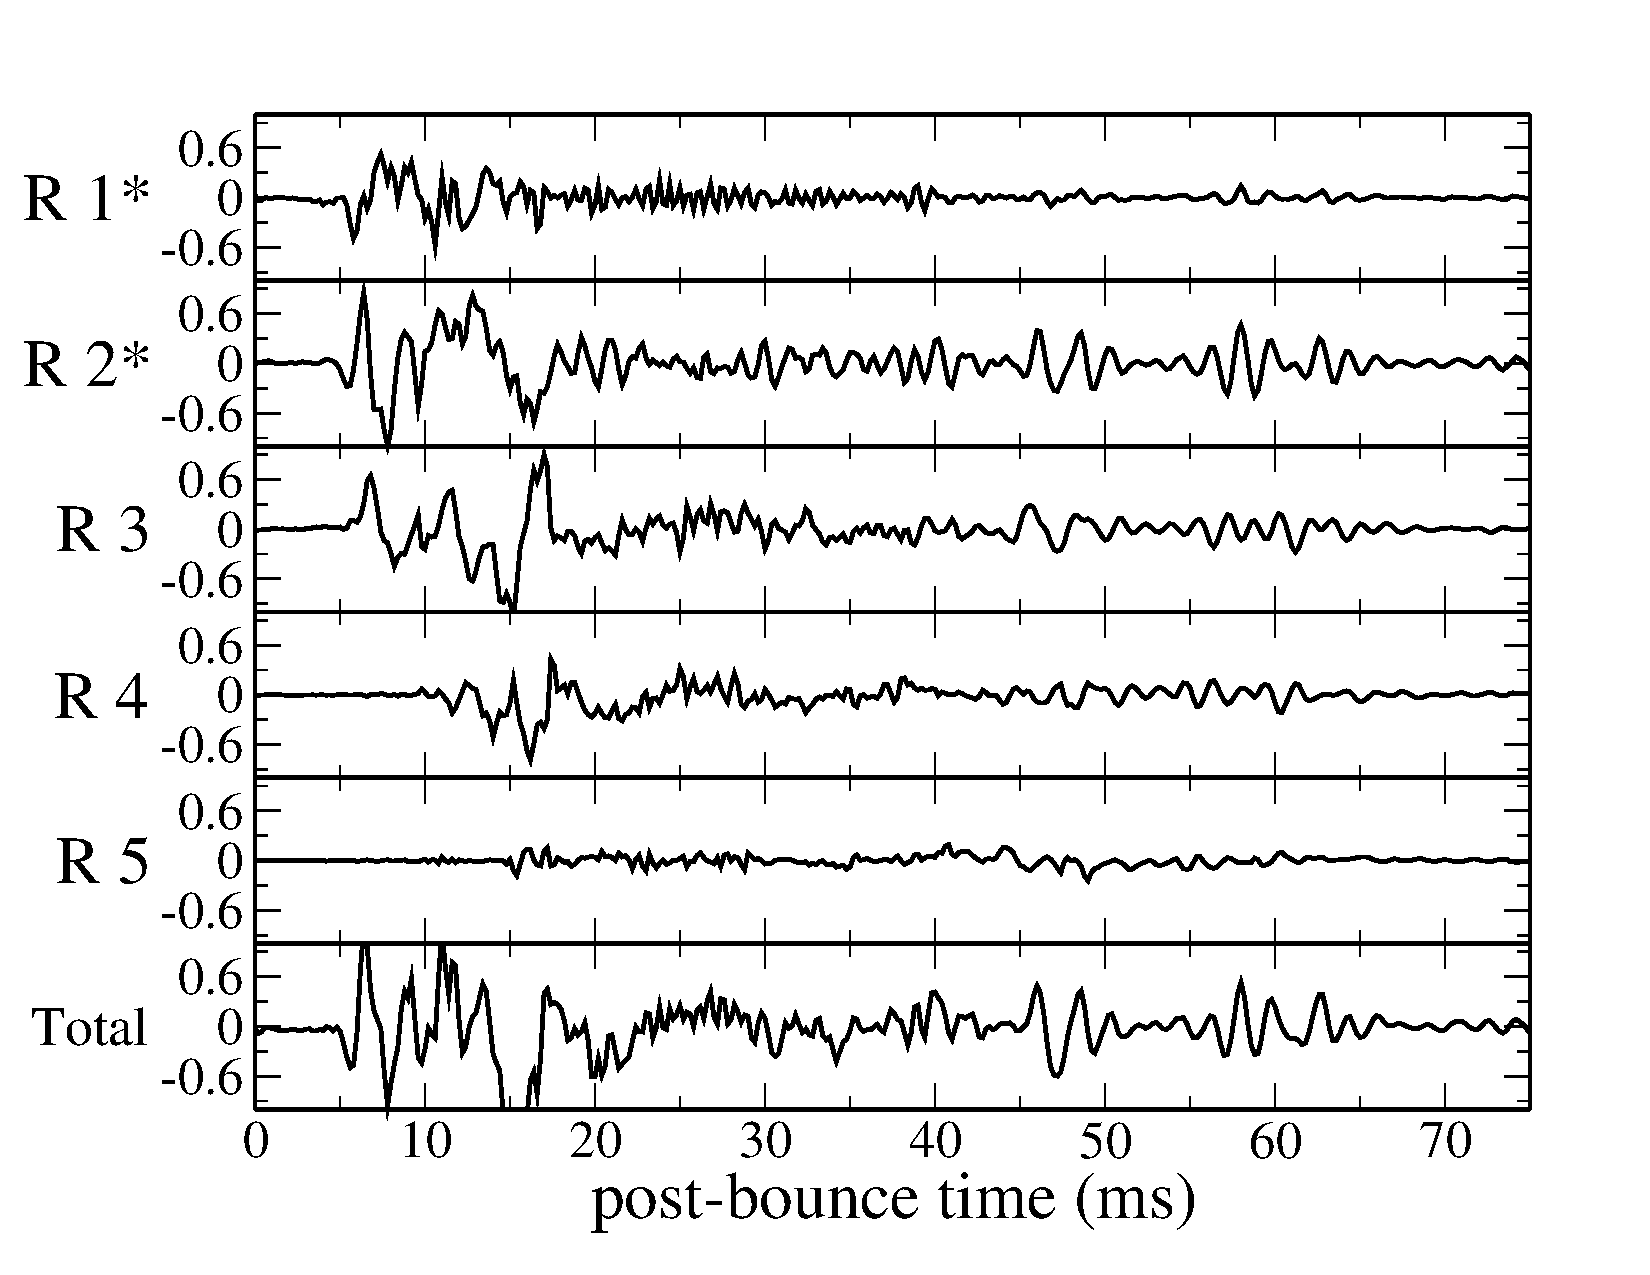
\includegraphics[width=1.0\textwidth]{Figures/D9.6_strain_byRegions.pdf}
      \end{figure}

    \column{.5\textwidth} % Right column and width
      \begin{figure}
        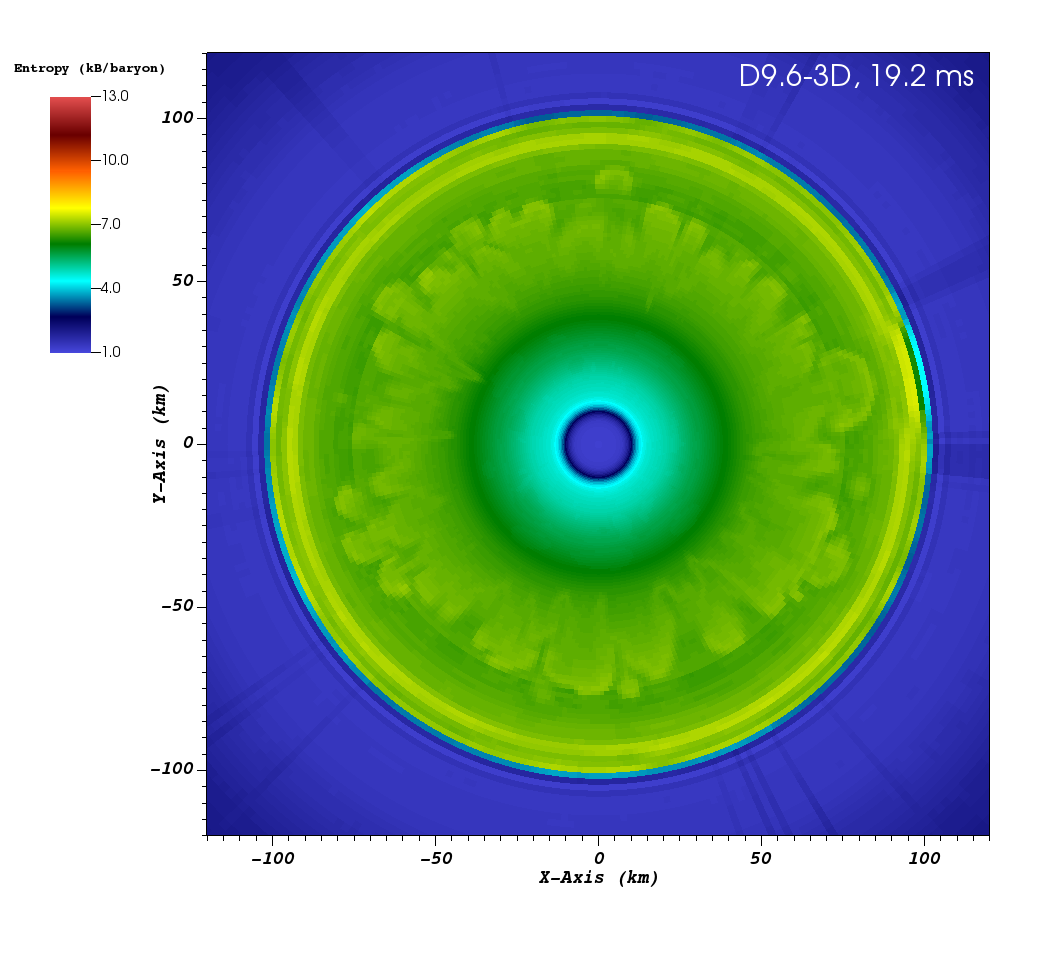
\includegraphics[width=1.0\textwidth]{Figures/D9.6_entropy_19.2ms.png}
      \end{figure}

  \end{columns}

\end{frame}

\begin{frame}

  \begin{columns}[c]

    \column{.5\textwidth} % Left column and width
      \begin{figure}
        \textbf{D15}
        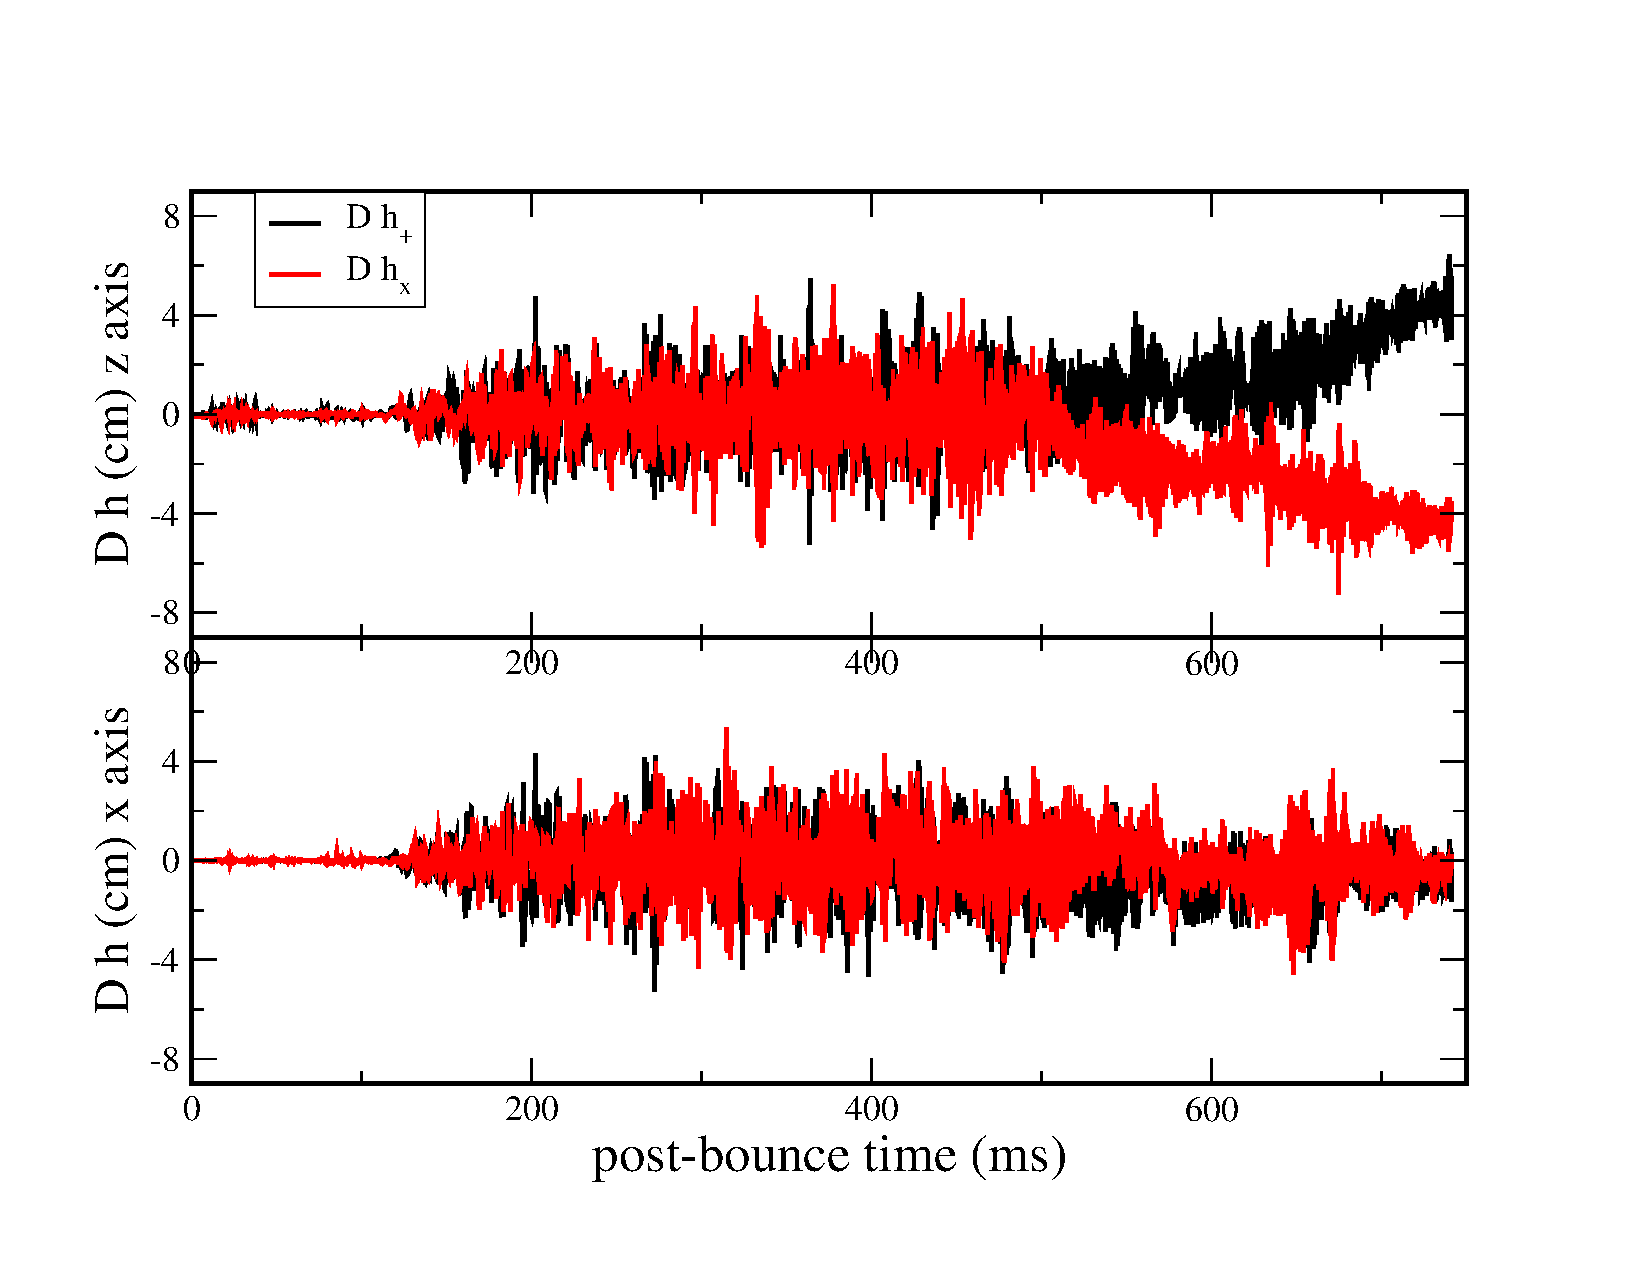
\includegraphics[width=1.0\textwidth]{Figures/D15_strain.pdf}
      \end{figure}

    \column{.5\textwidth} % Right column and width
      \begin{figure}
        \textbf{D25}
        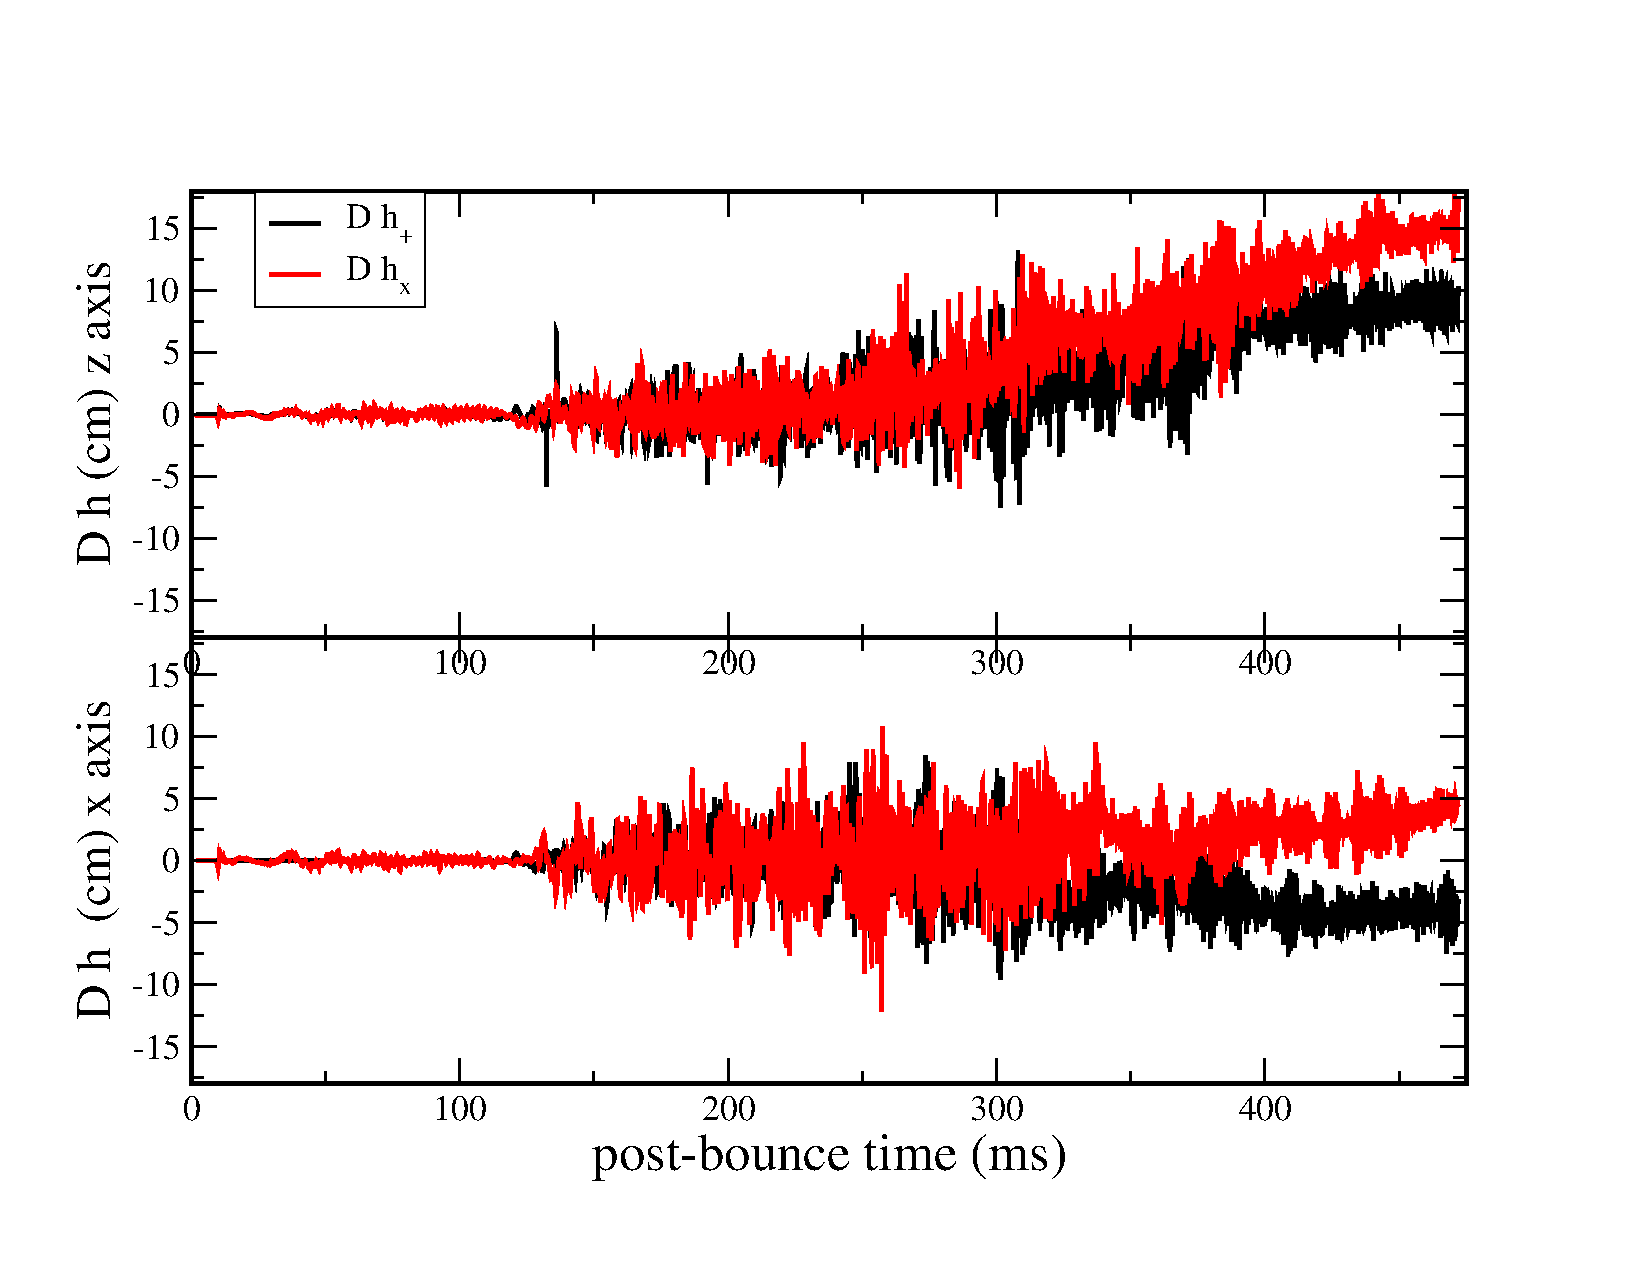
\includegraphics[width=1.0\textwidth]{Figures/D25_strain.pdf}
      \end{figure}

  \end{columns}

\end{frame}

\begin{frame}

  \begin{columns}[c]

    \column{.5\textwidth} % Left column and width
      \begin{figure}
        \textbf{D15}
        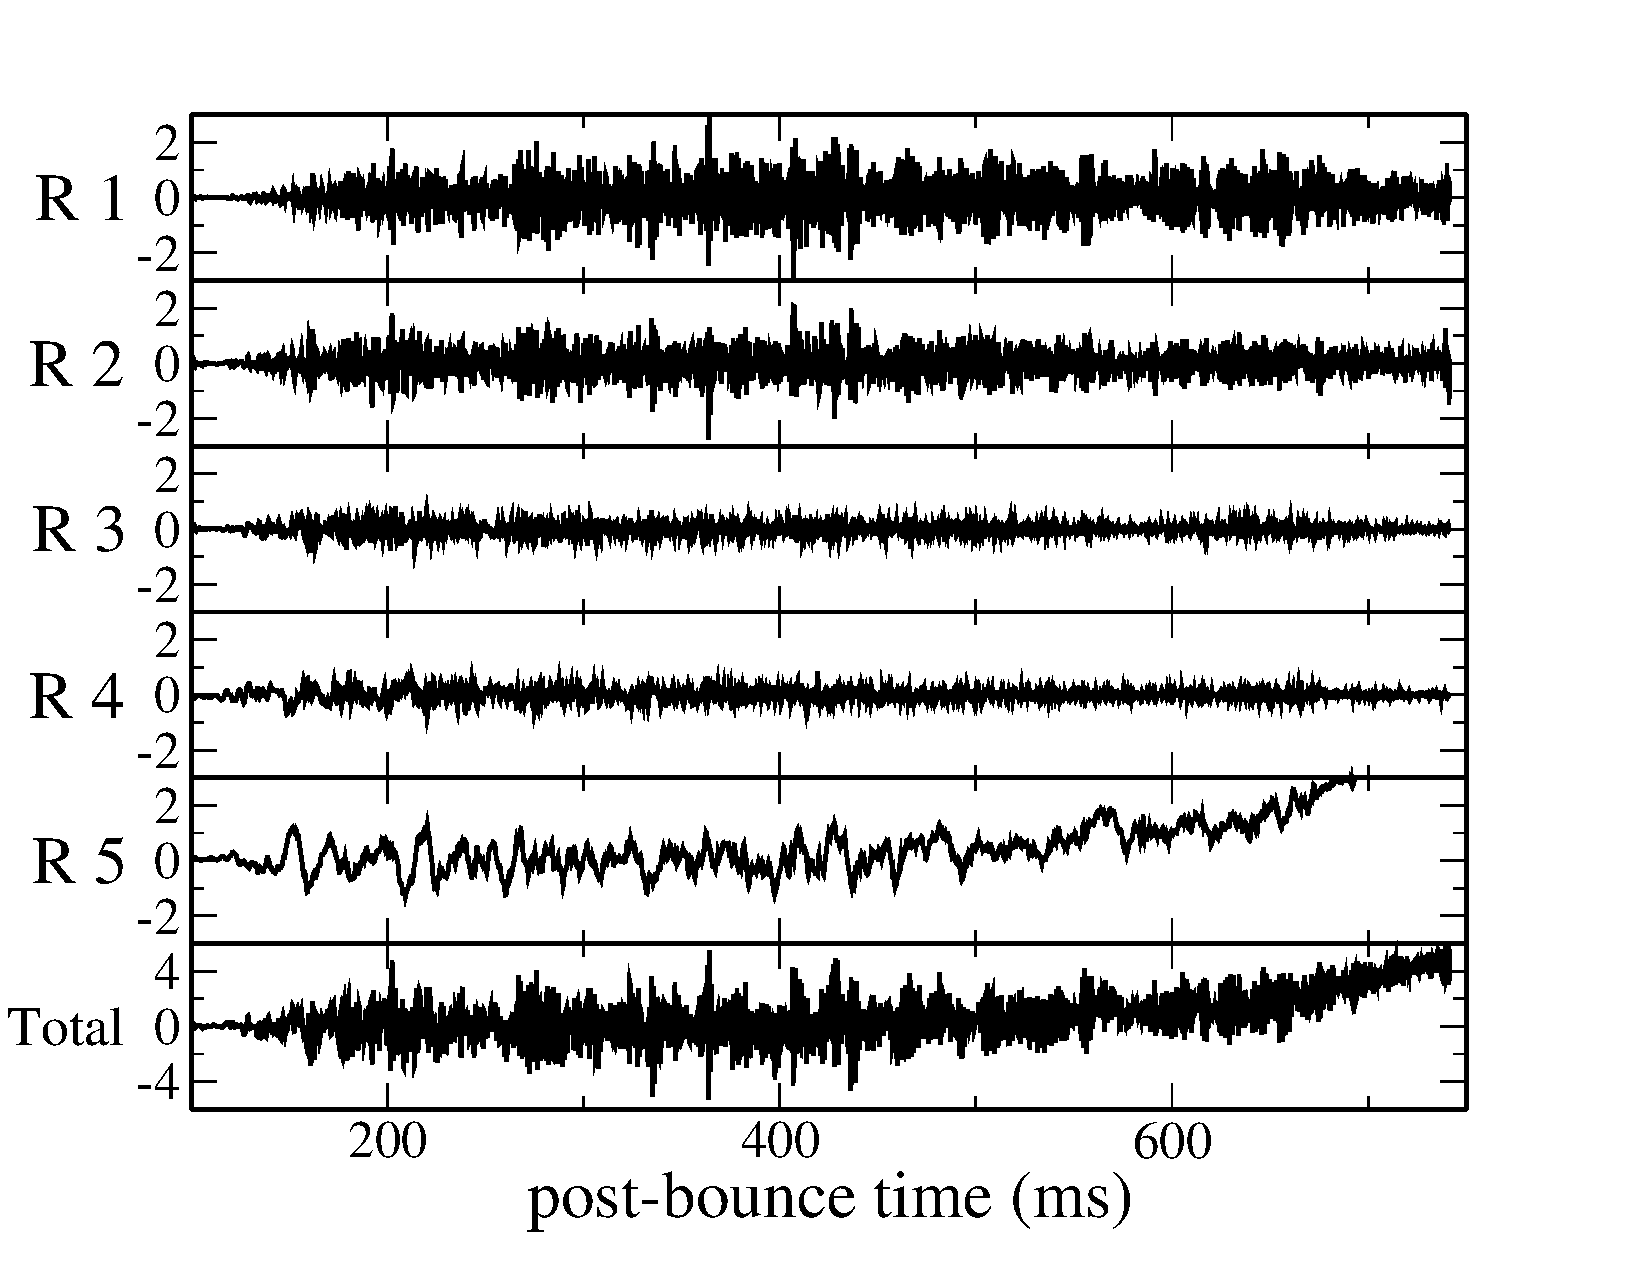
\includegraphics[width=1.0\textwidth]{Figures/D15_strain_byRegions.pdf}
      \end{figure}

    \column{.5\textwidth} % Right column and width
      \begin{figure}
        \textbf{D25}
        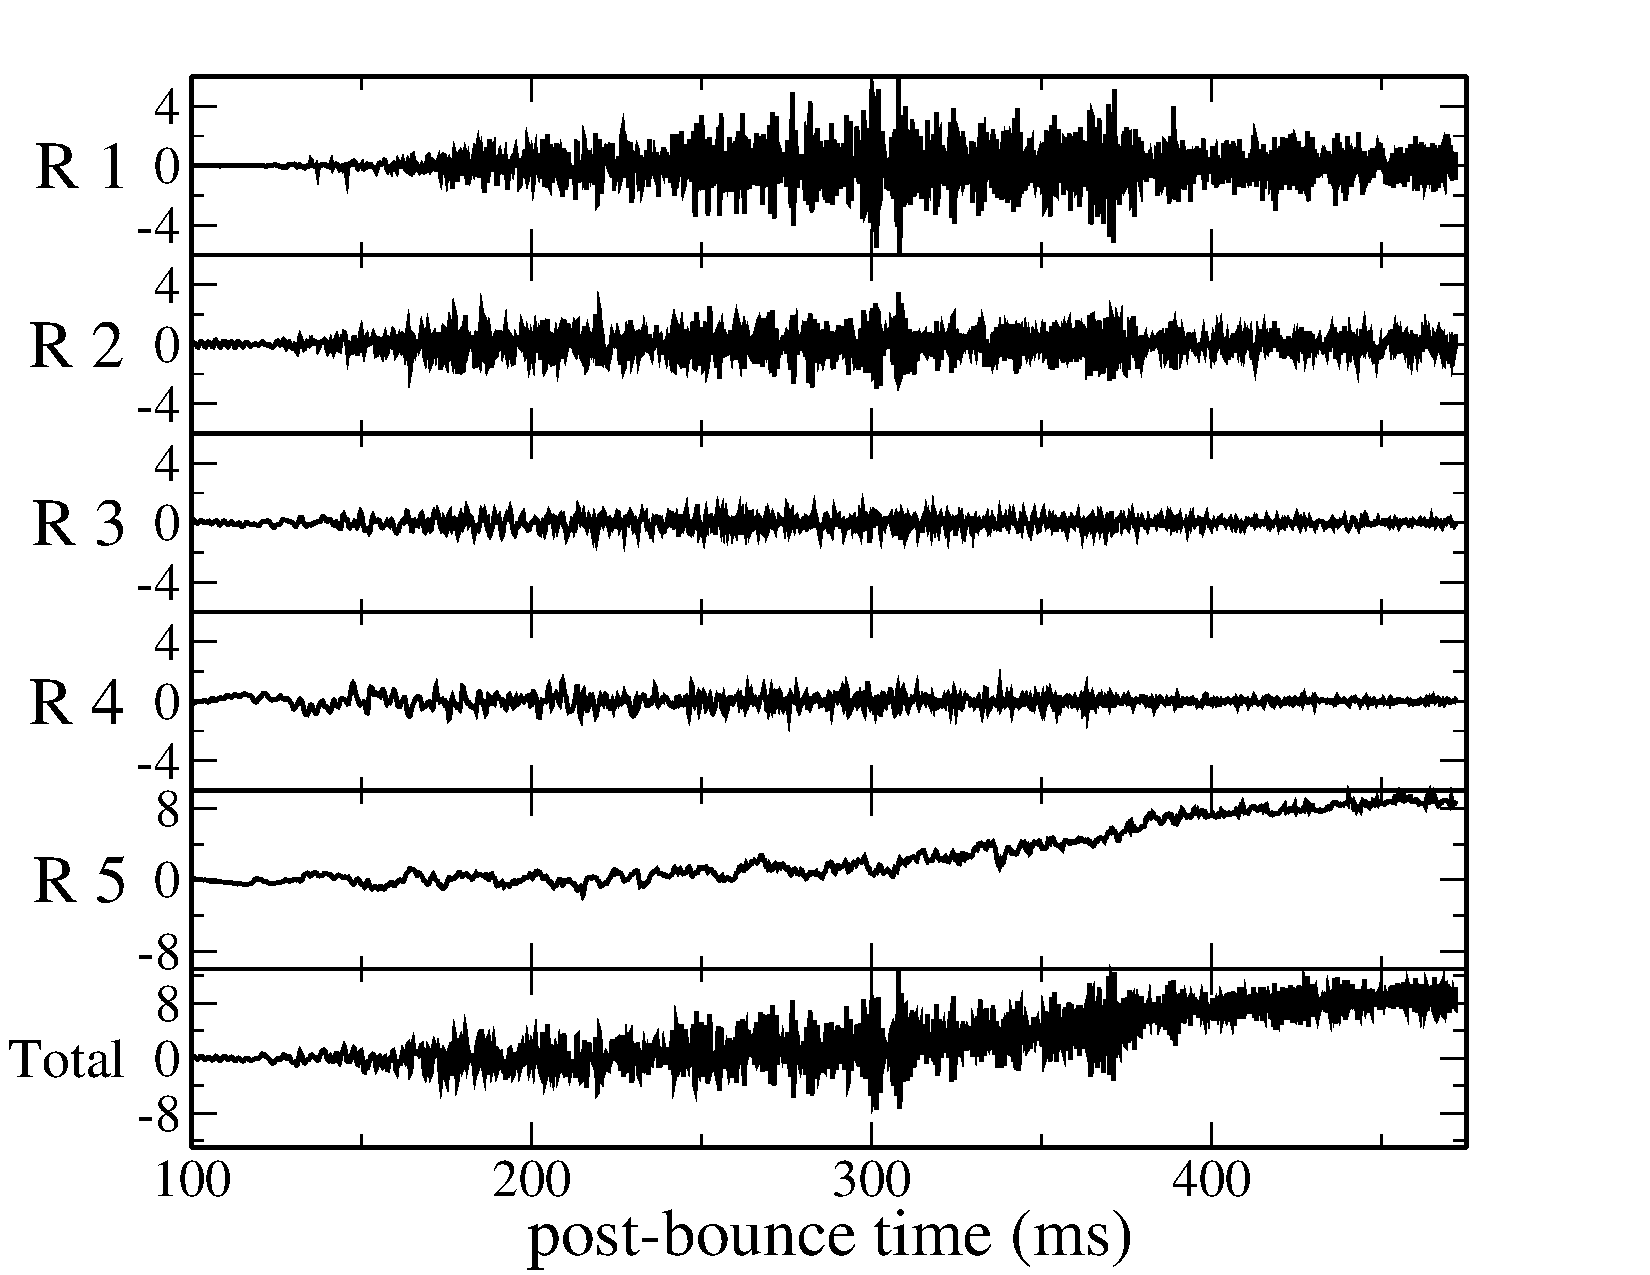
\includegraphics[width=1.0\textwidth]{Figures/D25_strain_byRegions.pdf}
      \end{figure}

  \end{columns}

\end{frame}

\subsection{Spectrograms}

\begin{frame}

  \begin{columns}[c]

    \column{.33\textwidth}
      \begin{figure}
        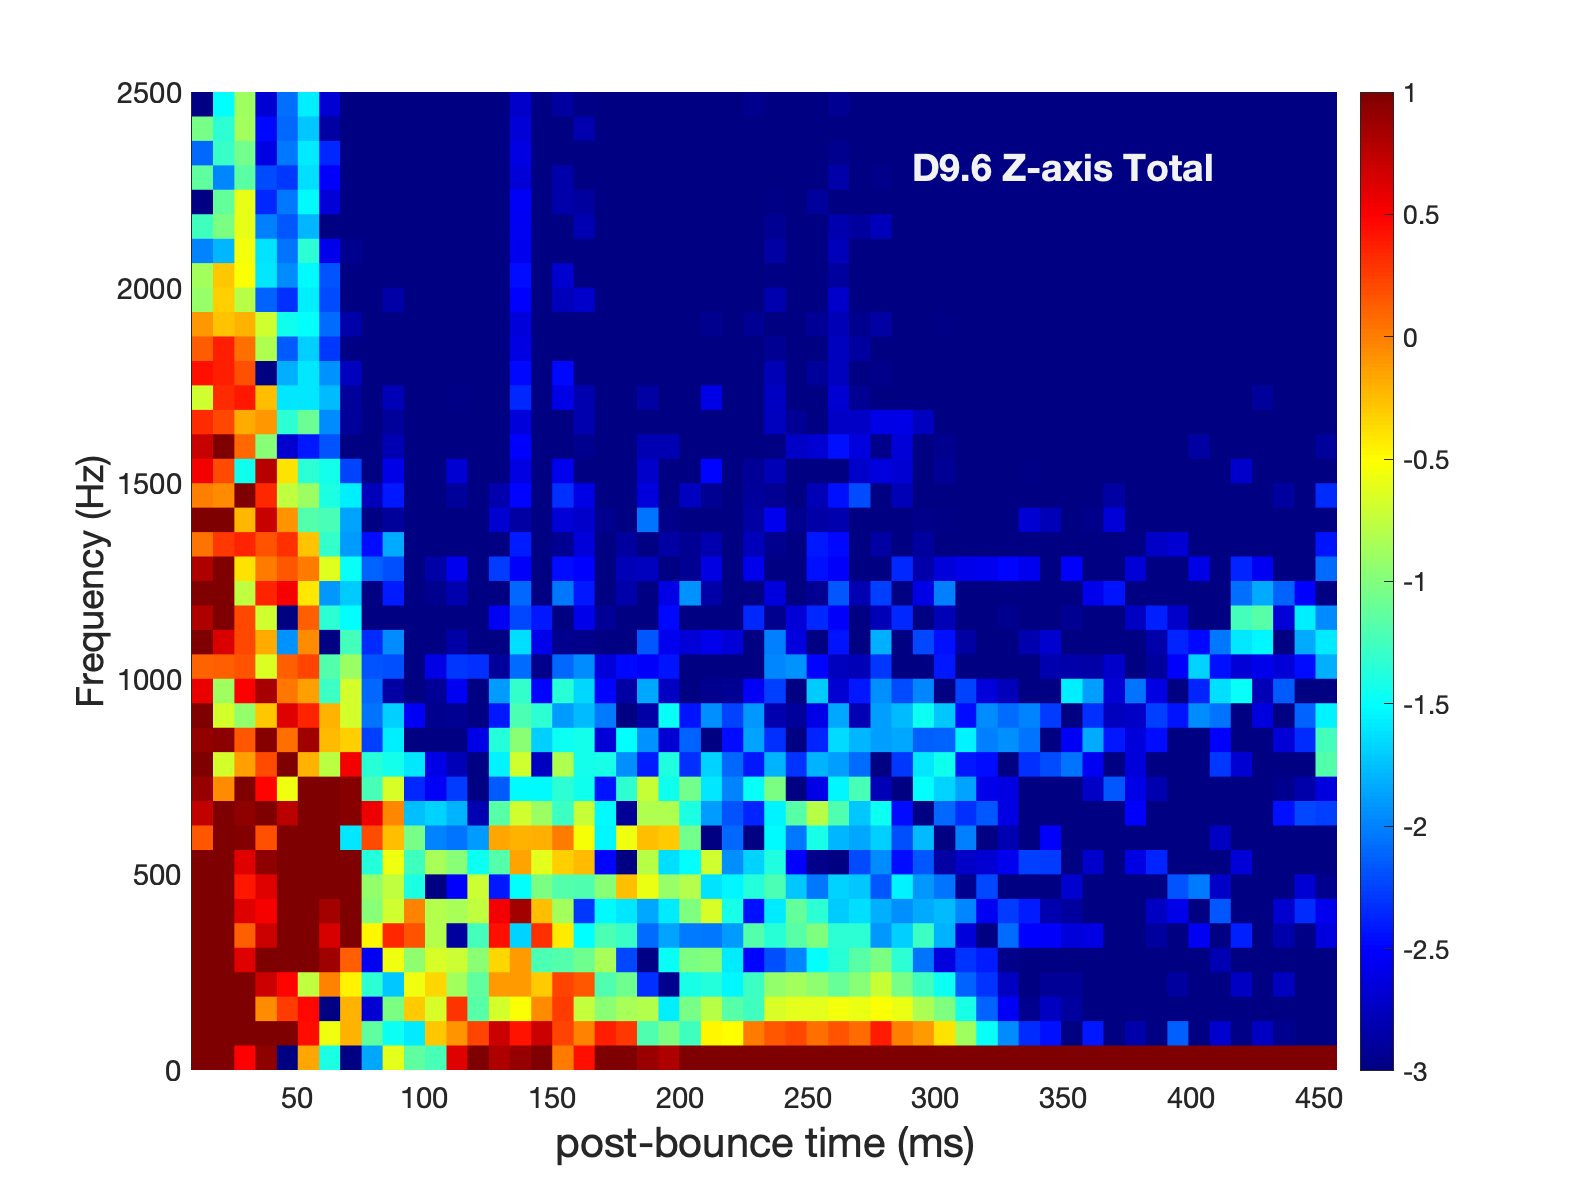
\includegraphics[width=1.0\textwidth]{Figures/D9.6_spectrogram_TOTAL.pdf}
      \end{figure}

    \column{.33\textwidth}
      \begin{figure}
        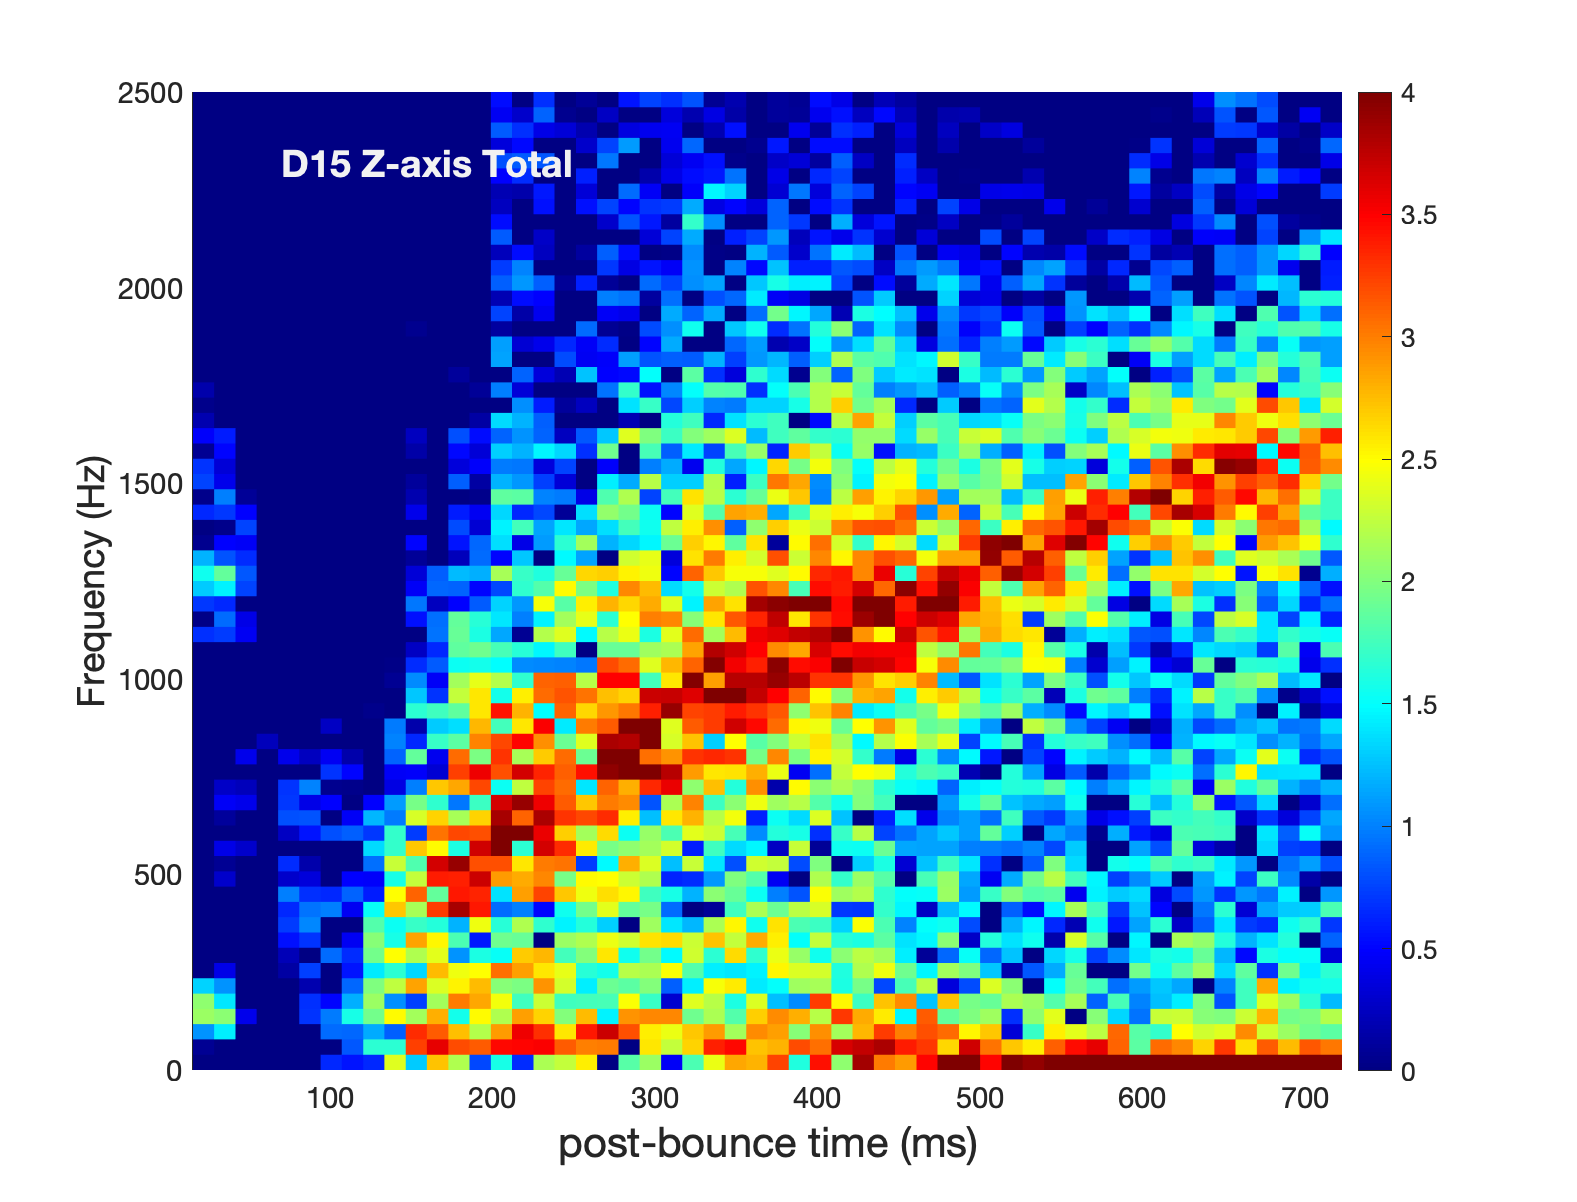
\includegraphics[width=1.0\textwidth]{Figures/D15_spectrogram_TOTAL.pdf}
      \end{figure}

    \column{.33\textwidth}
      \begin{figure}
        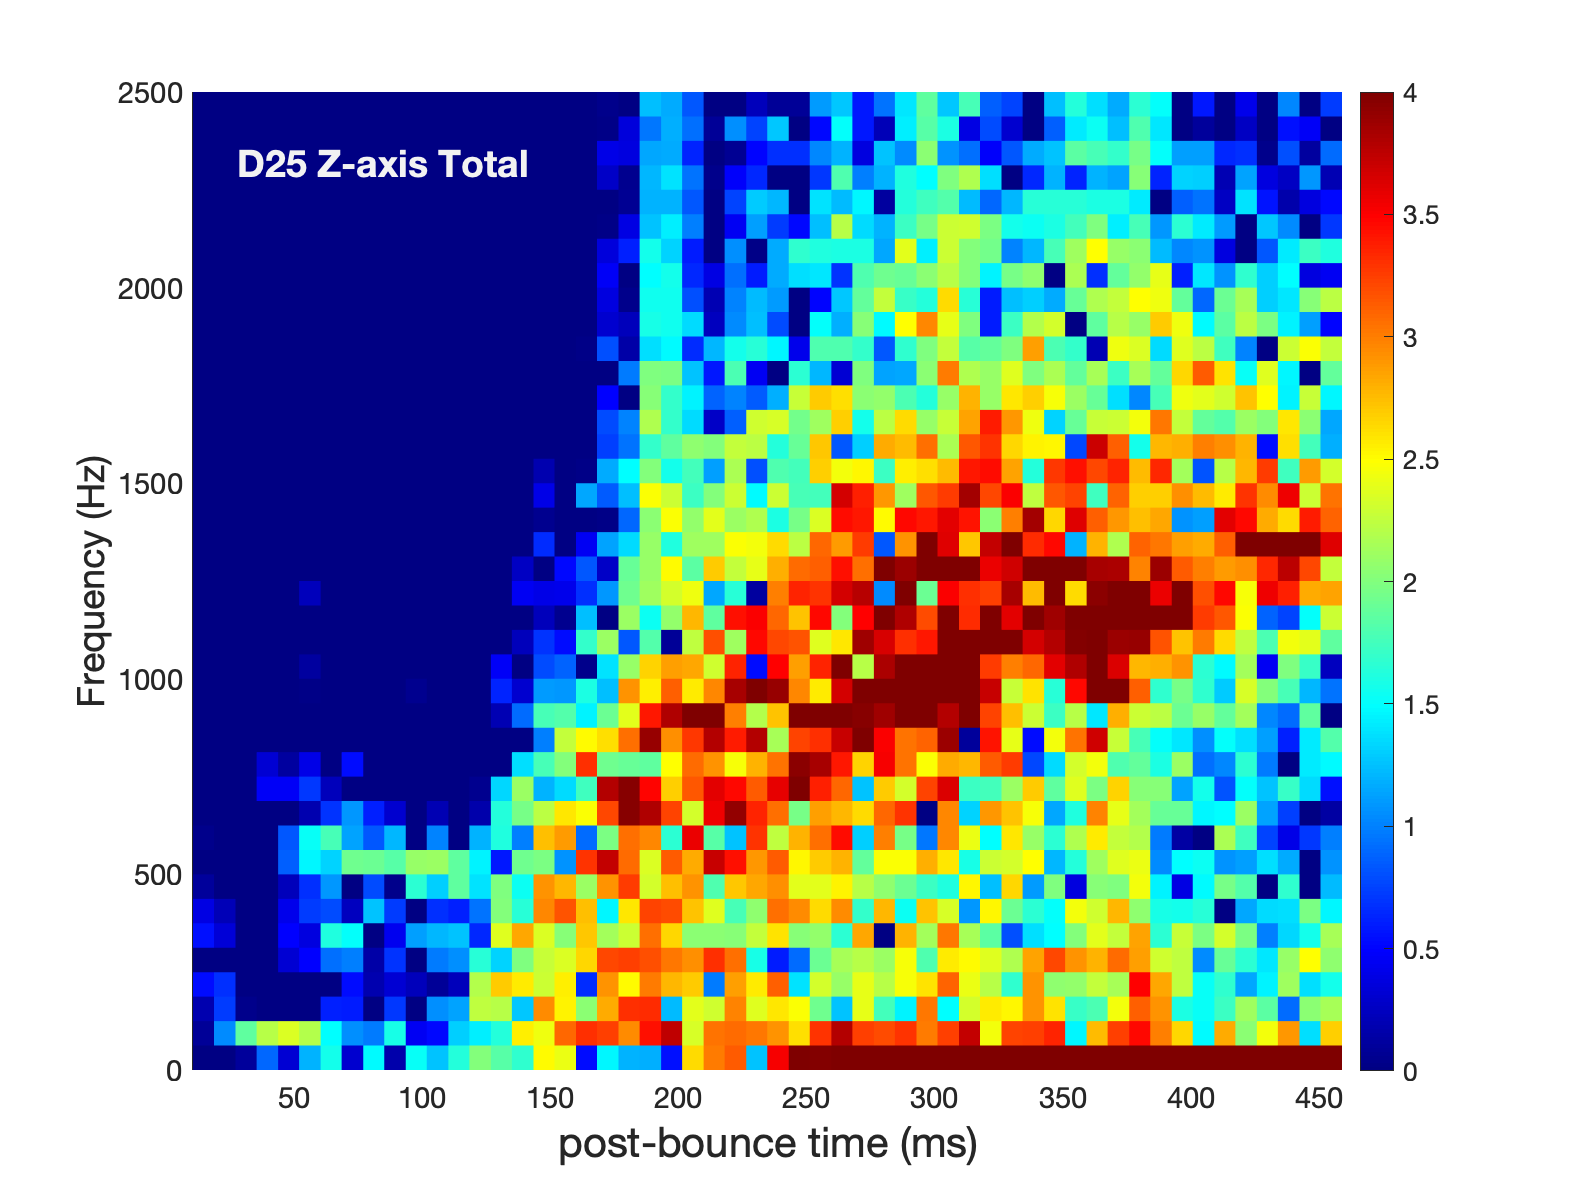
\includegraphics[width=1.0\textwidth]{Figures/D25_spectrogram_TOTAL.pdf}
      \end{figure}

  \end{columns}

\end{frame}

\begin{frame}

  \begin{figure}
    \centering
    \subfloat{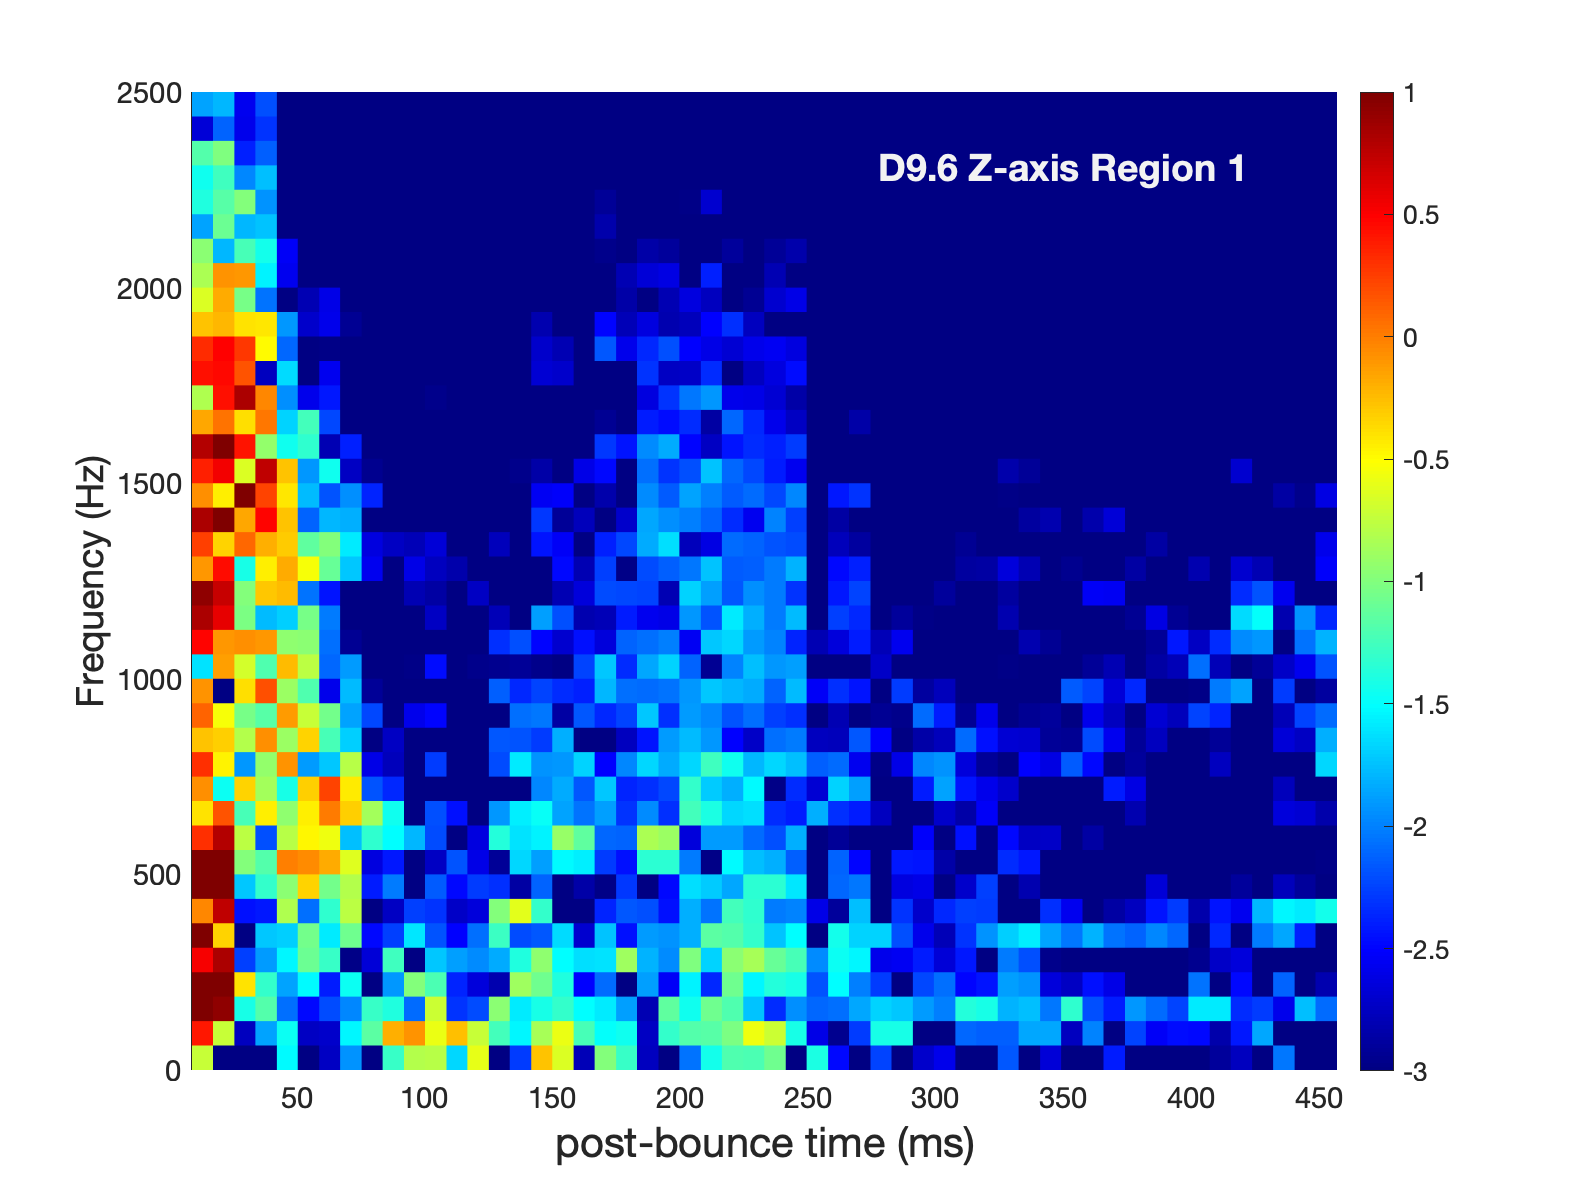
\includegraphics[width=0.25\textwidth]{Figures/D9.6_spectrogram_region01.pdf}}
    \subfloat{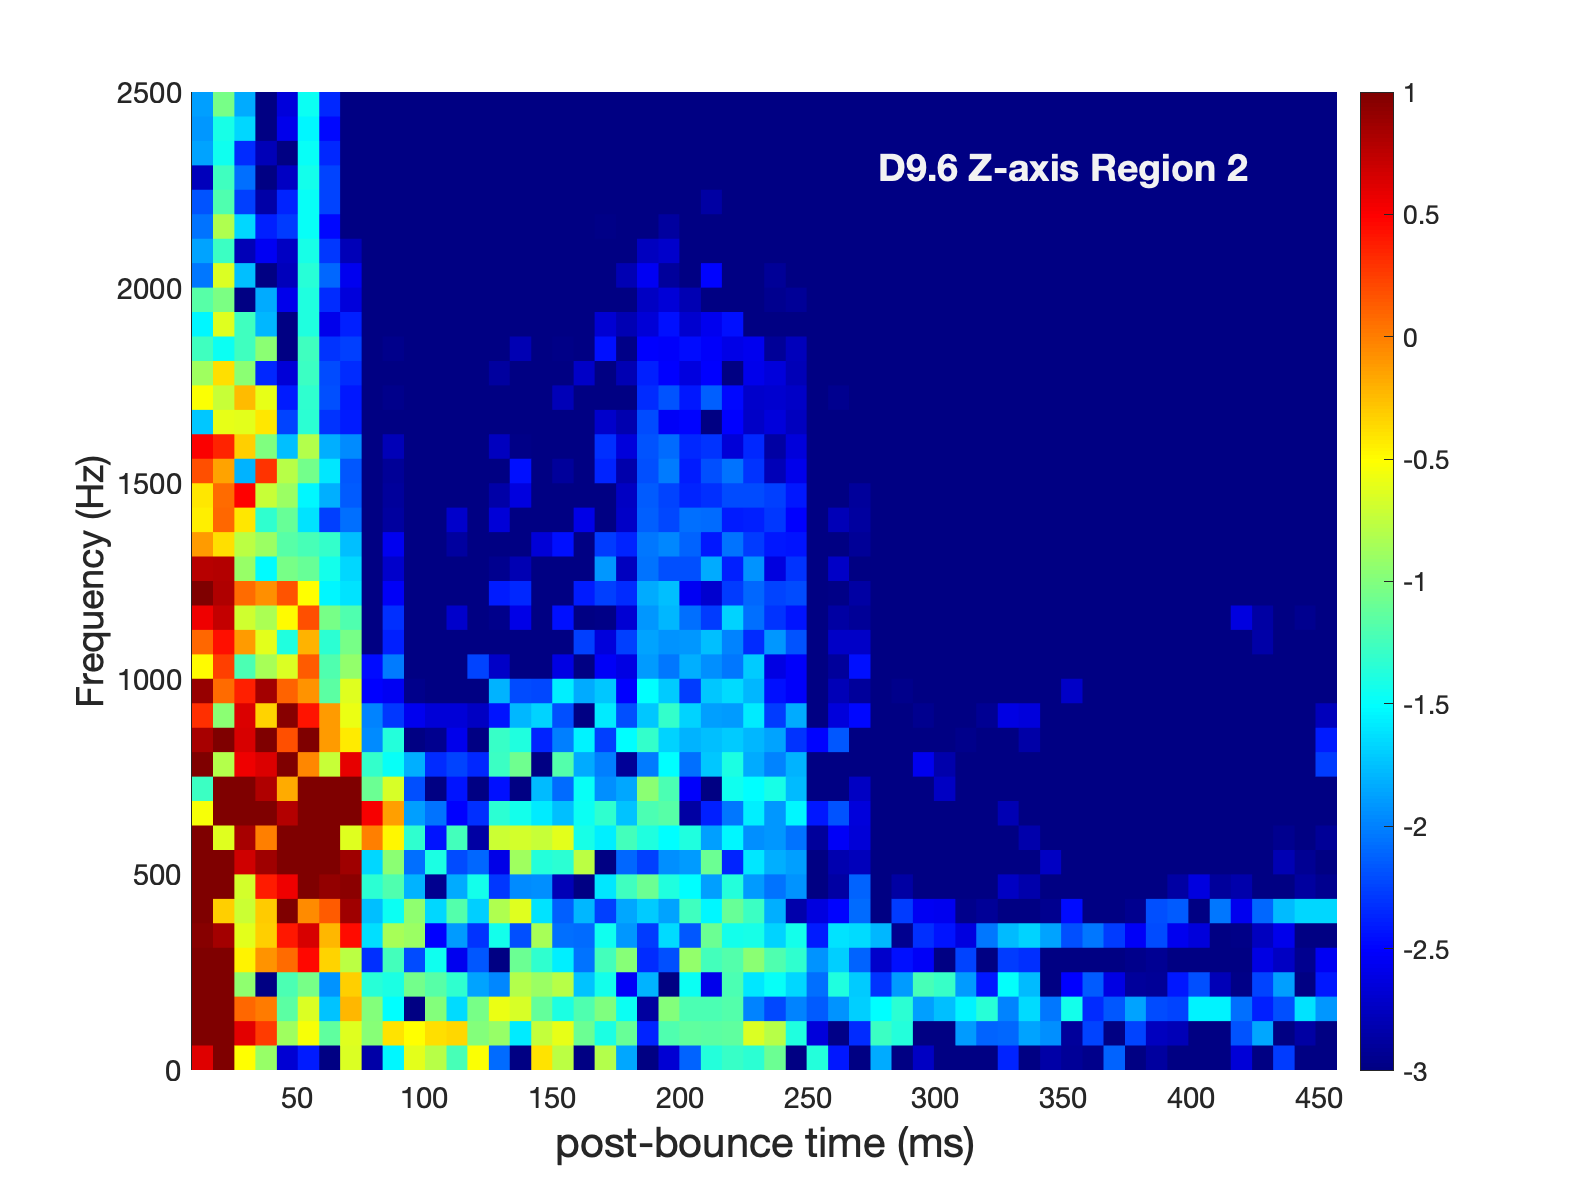
\includegraphics[width=0.25\textwidth]{Figures/D9.6_spectrogram_region02.pdf}}
    \subfloat{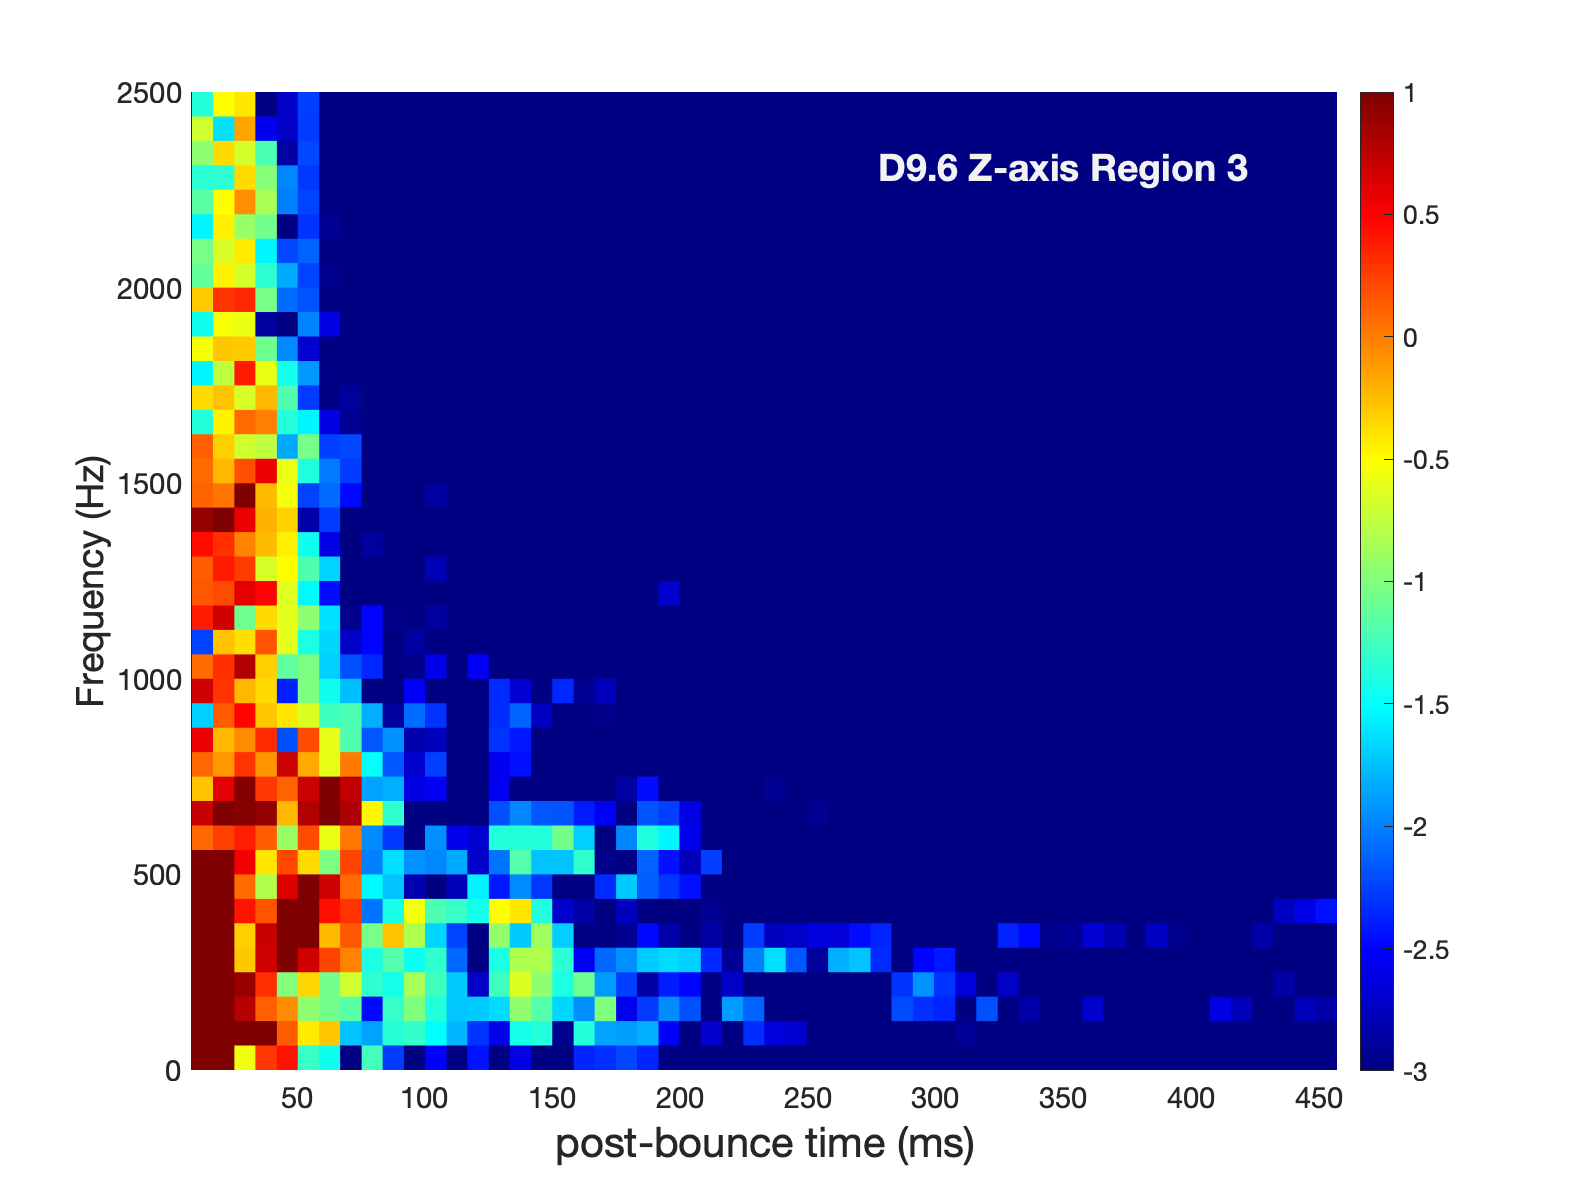
\includegraphics[width=0.25\textwidth]{Figures/D9.6_spectrogram_region03.pdf}}
  \end{figure}
  \vspace{-2em}
  \begin{figure}
    \centering
    \subfloat{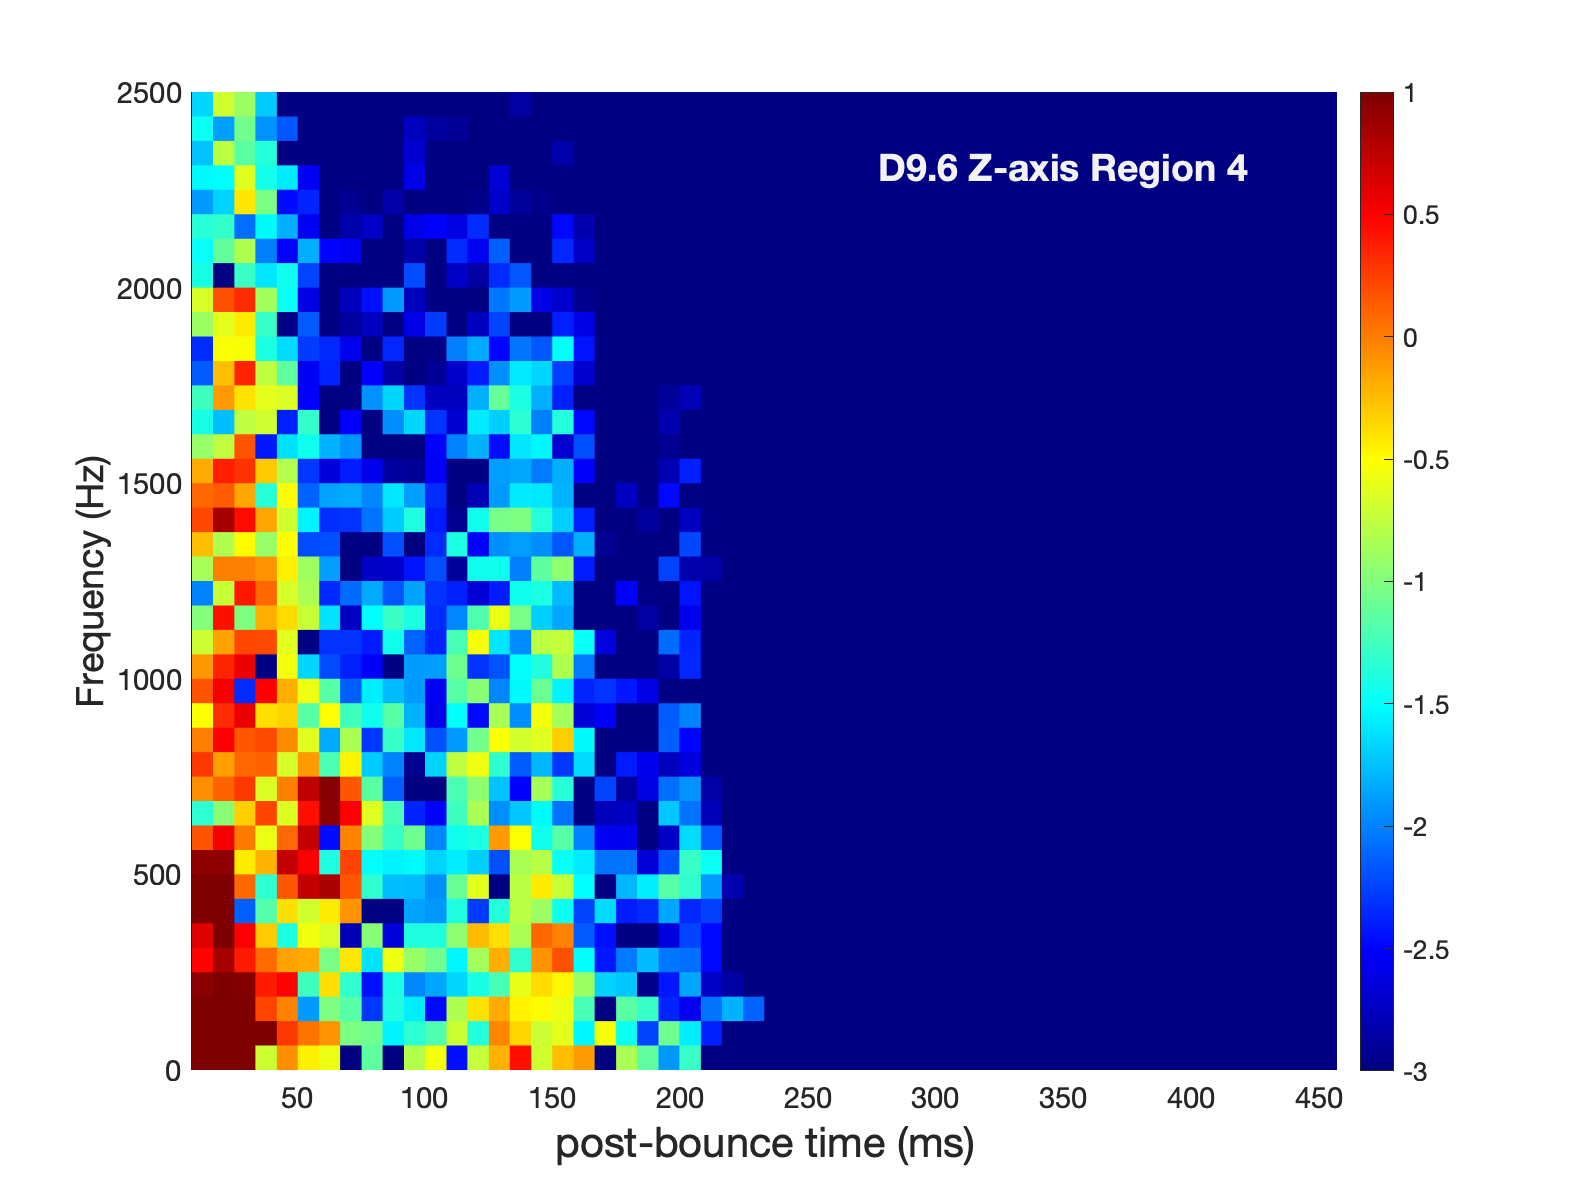
\includegraphics[width=0.25\textwidth]{Figures/D9.6_spectrogram_region04.pdf}}
    \subfloat{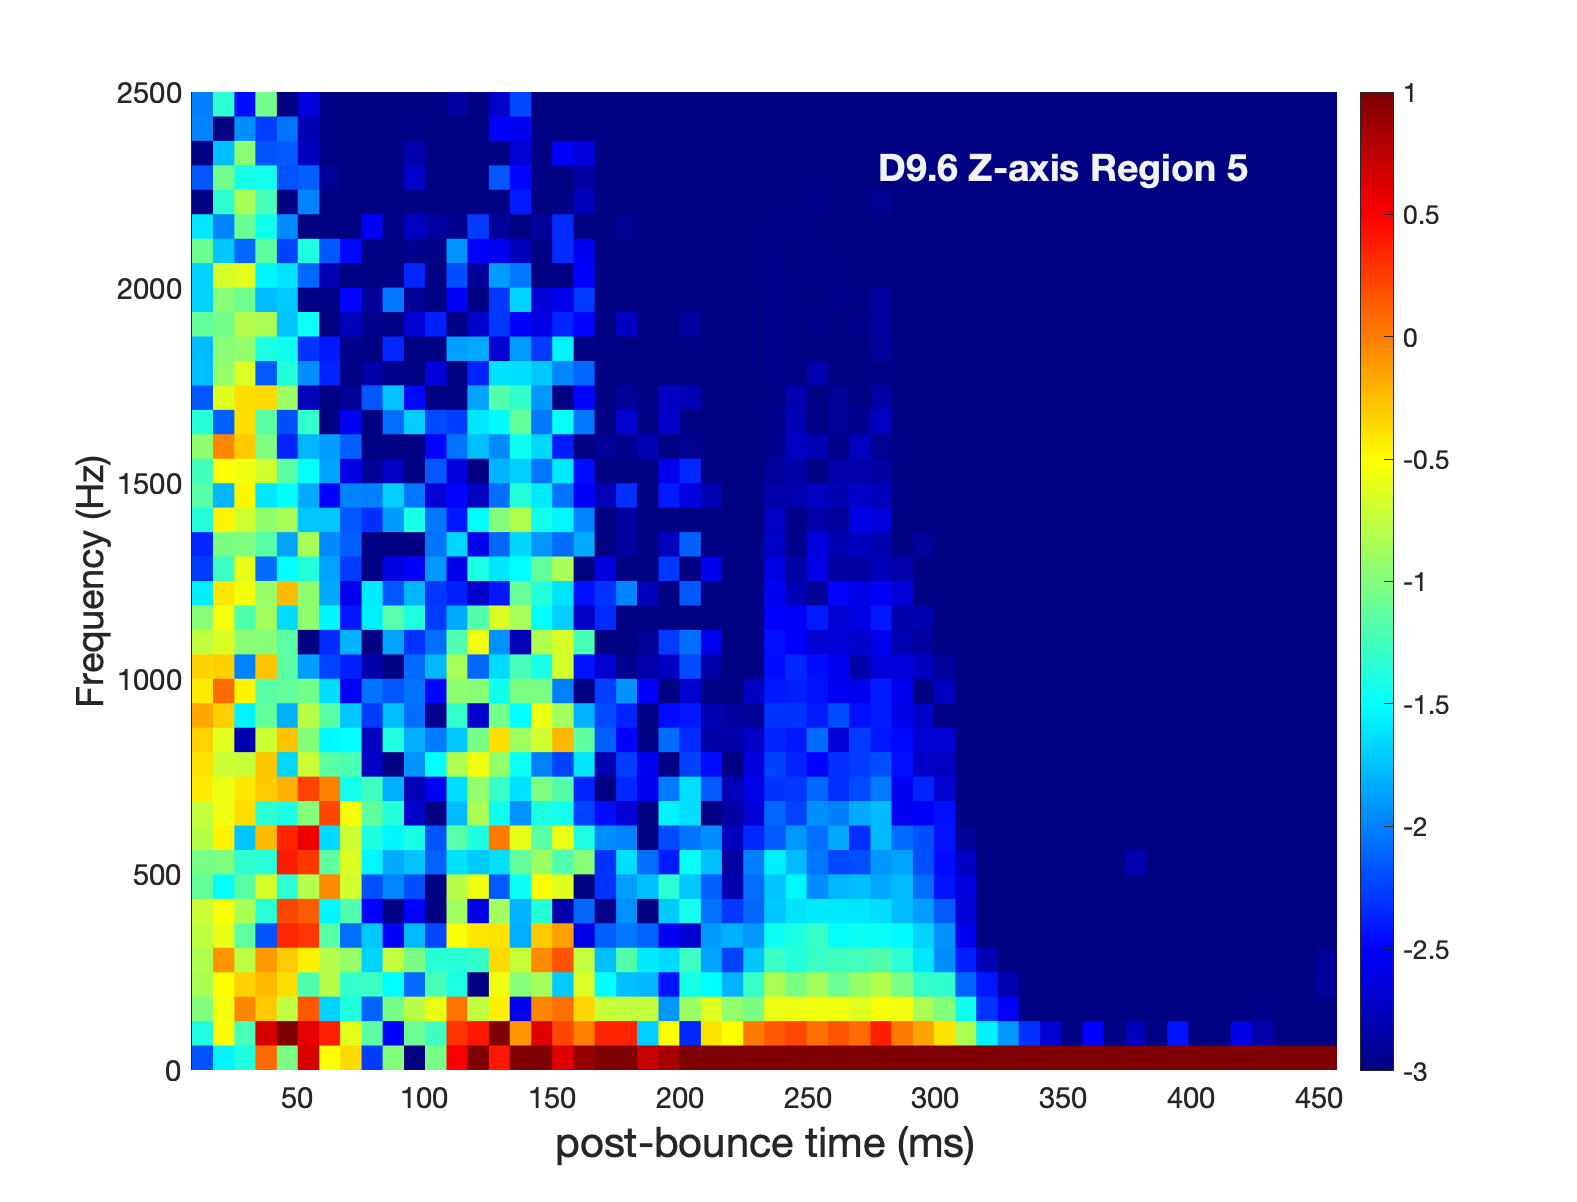
\includegraphics[width=0.25\textwidth]{Figures/D9.6_spectrogram_region05.pdf}}
    \subfloat{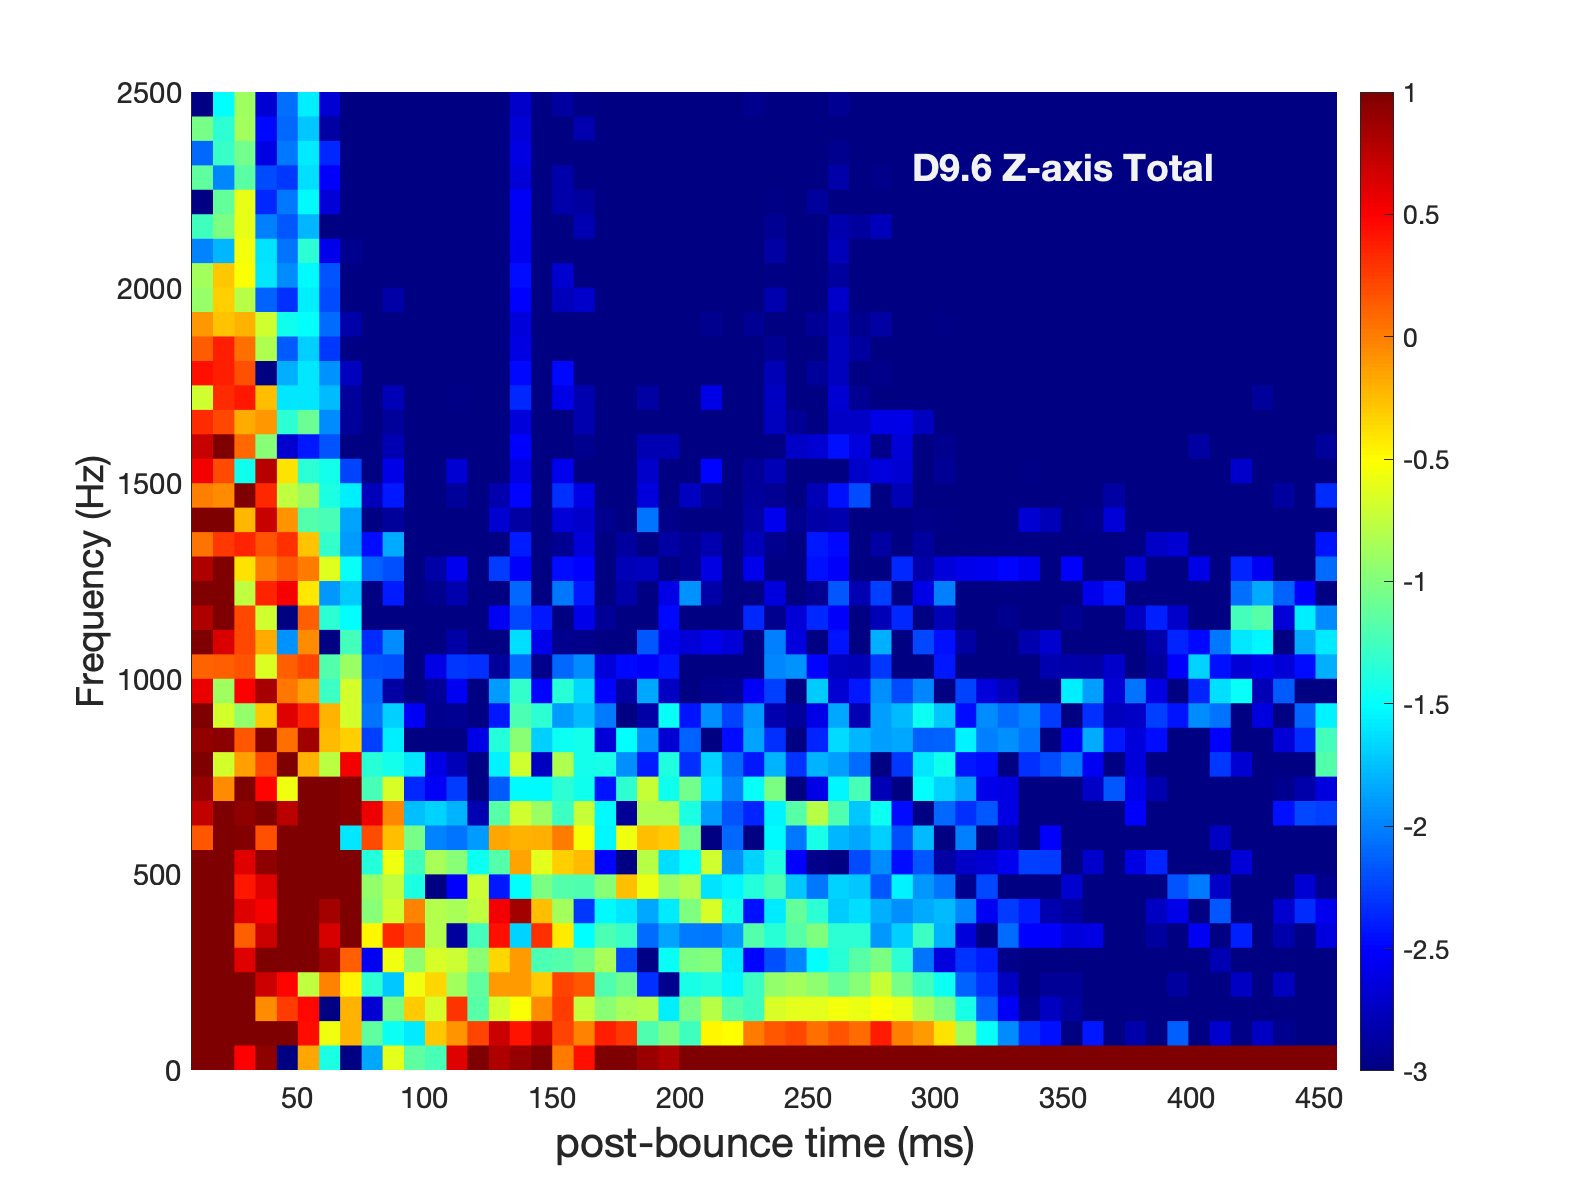
\includegraphics[width=0.25\textwidth]{Figures/D9.6_spectrogram_TOTAL.pdf}}
  \end{figure}

\end{frame}

\begin{frame}

  \begin{figure}
    \centering
    \subfloat{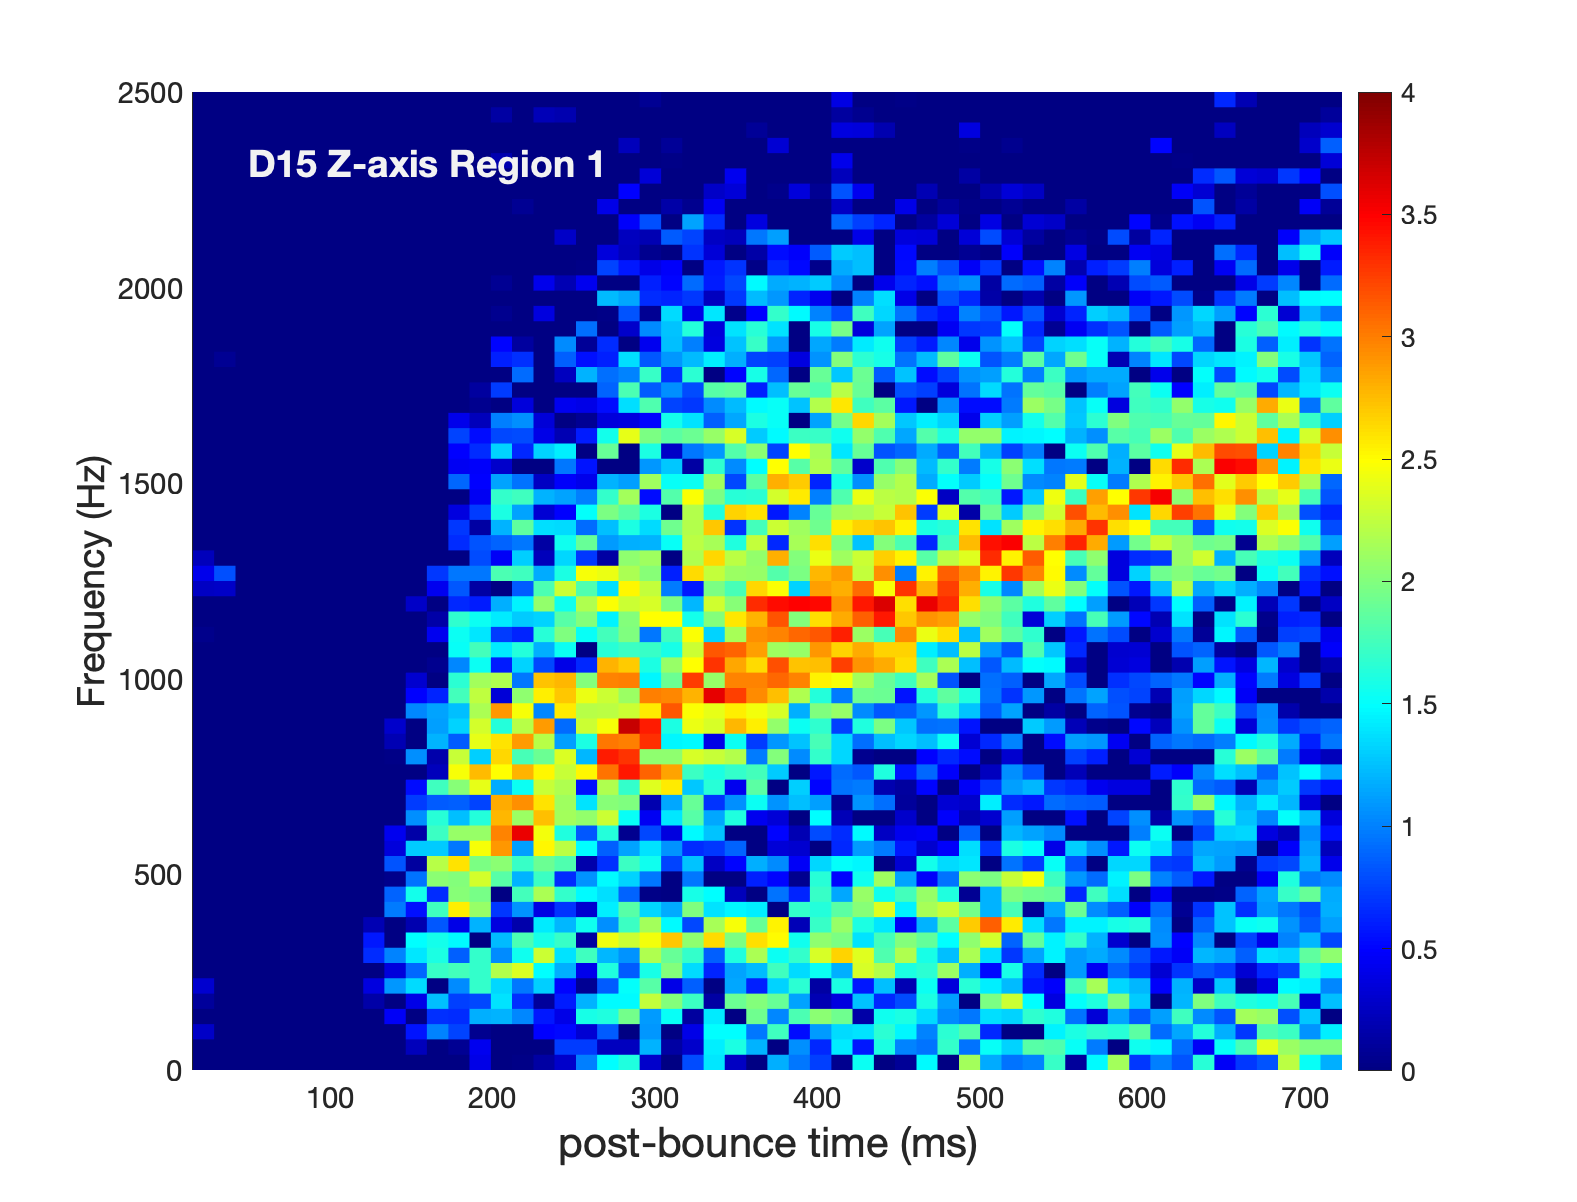
\includegraphics[width=0.25\textwidth]{Figures/D15_spectrogram_region01.pdf}}
    \subfloat{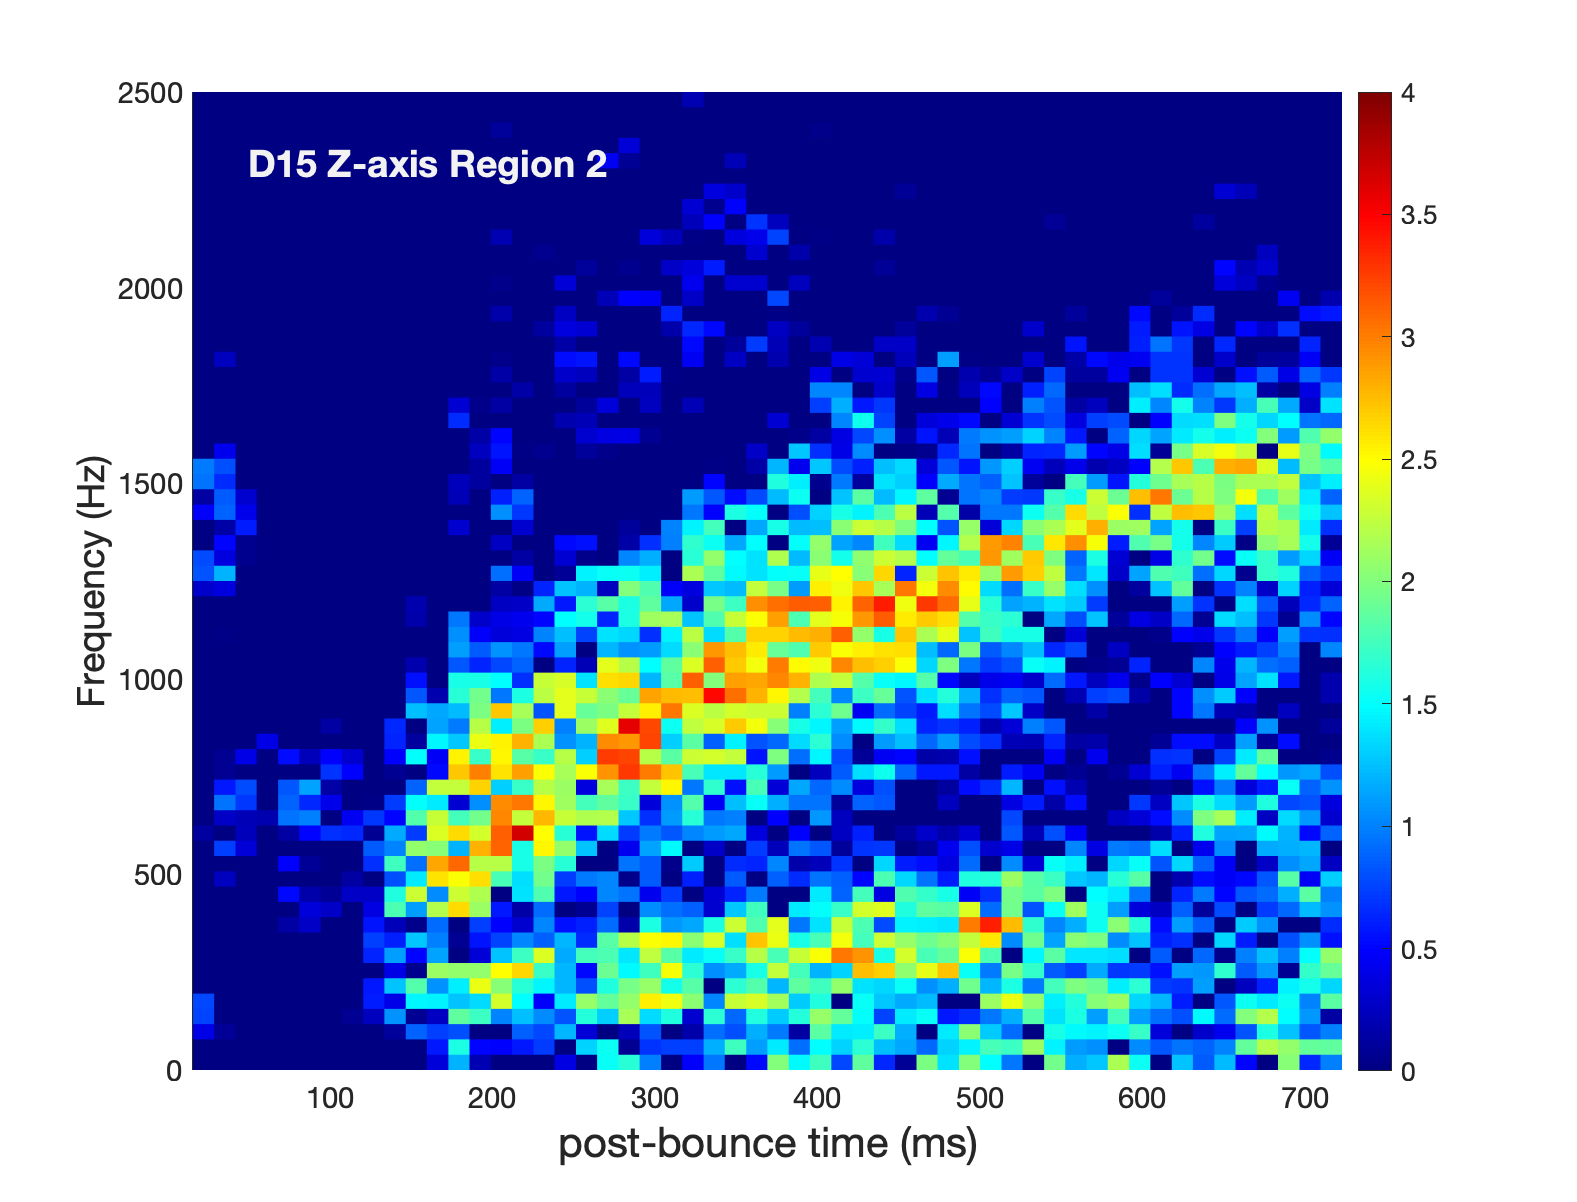
\includegraphics[width=0.25\textwidth]{Figures/D15_spectrogram_region02.pdf}}
    \subfloat{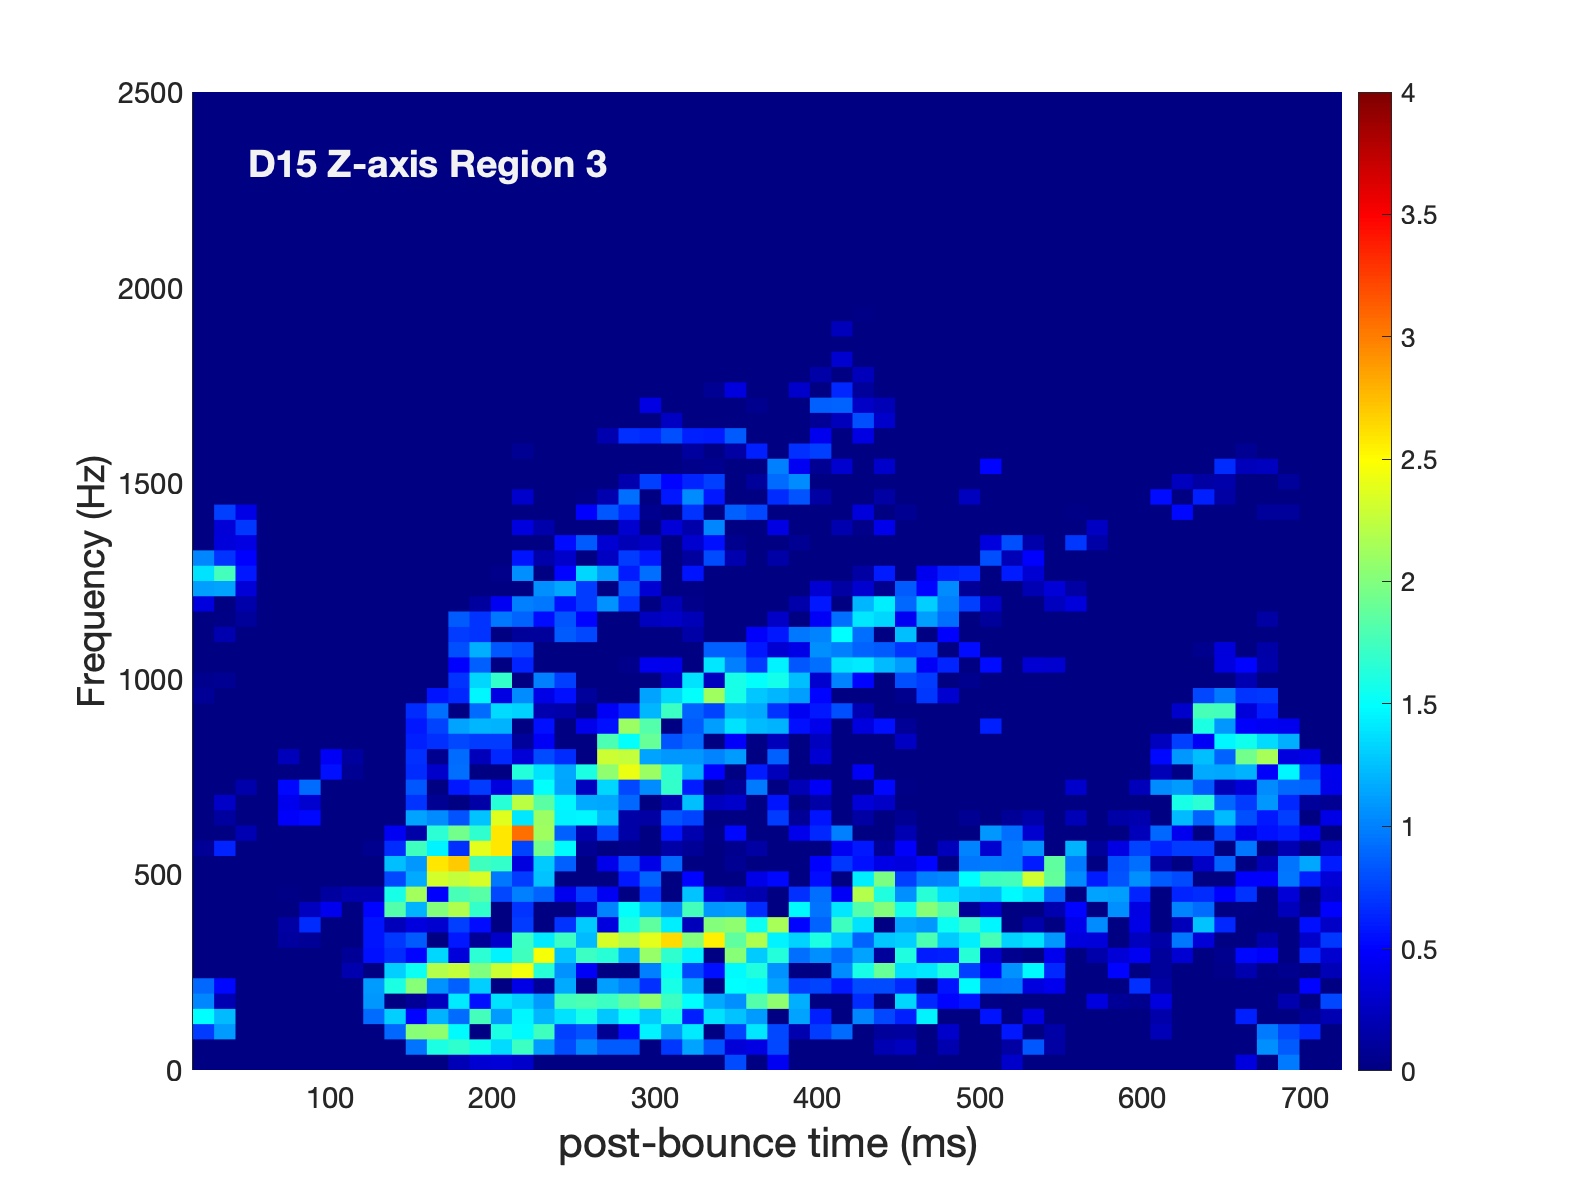
\includegraphics[width=0.25\textwidth]{Figures/D15_spectrogram_region03.pdf}}
  \end{figure}
  \vspace{-2em}
  \begin{figure}
    \centering
    \subfloat{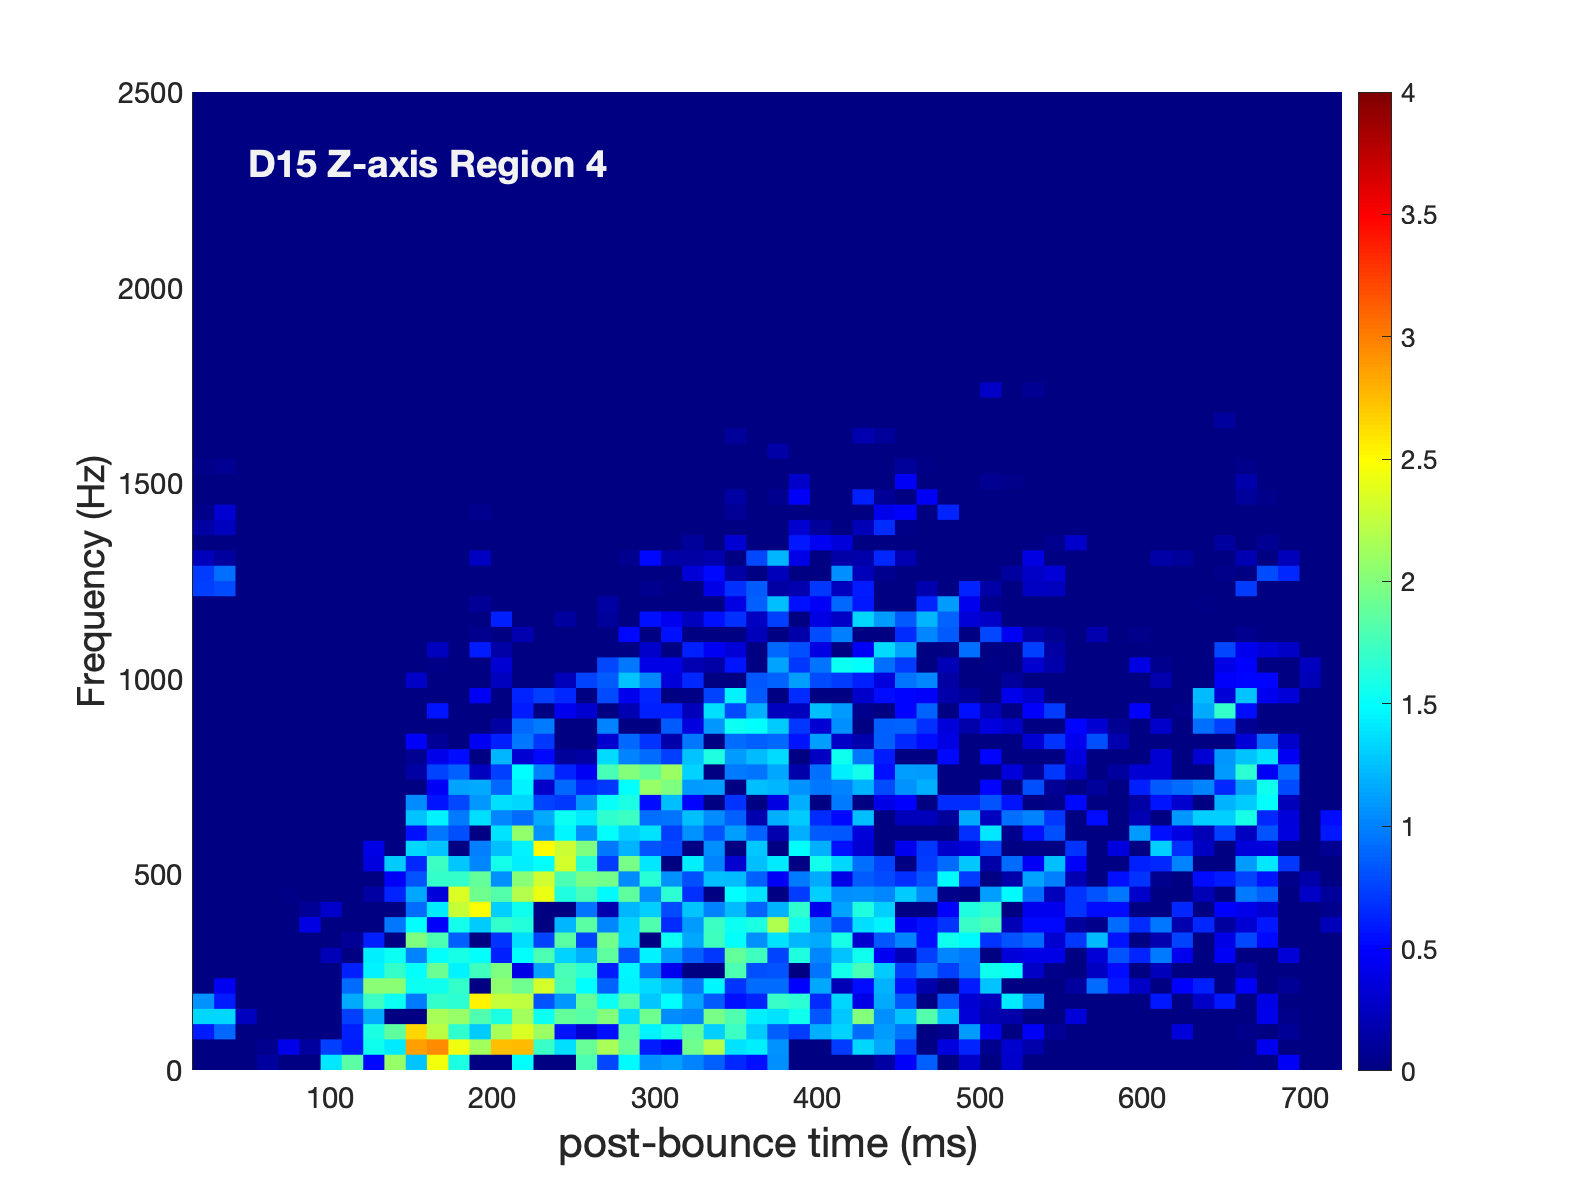
\includegraphics[width=0.25\textwidth]{Figures/D15_spectrogram_region04.pdf}}
    \subfloat{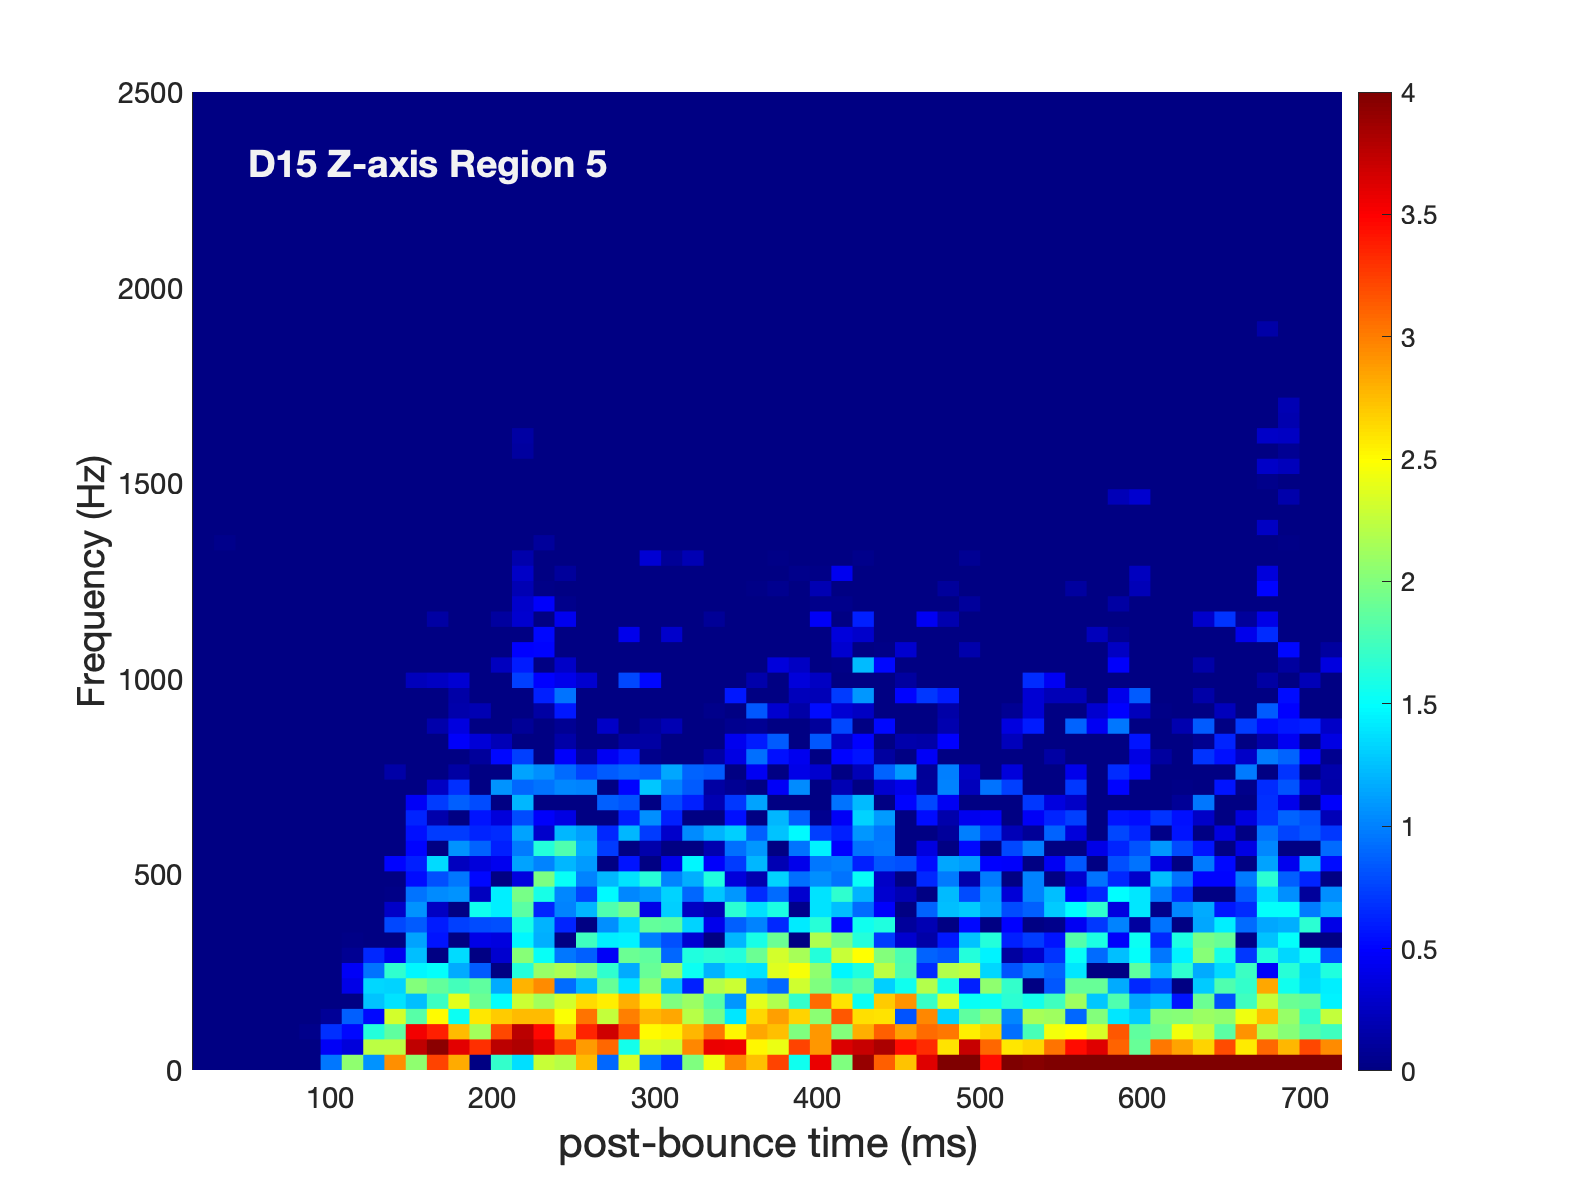
\includegraphics[width=0.25\textwidth]{Figures/D15_spectrogram_region05.pdf}}
    \subfloat{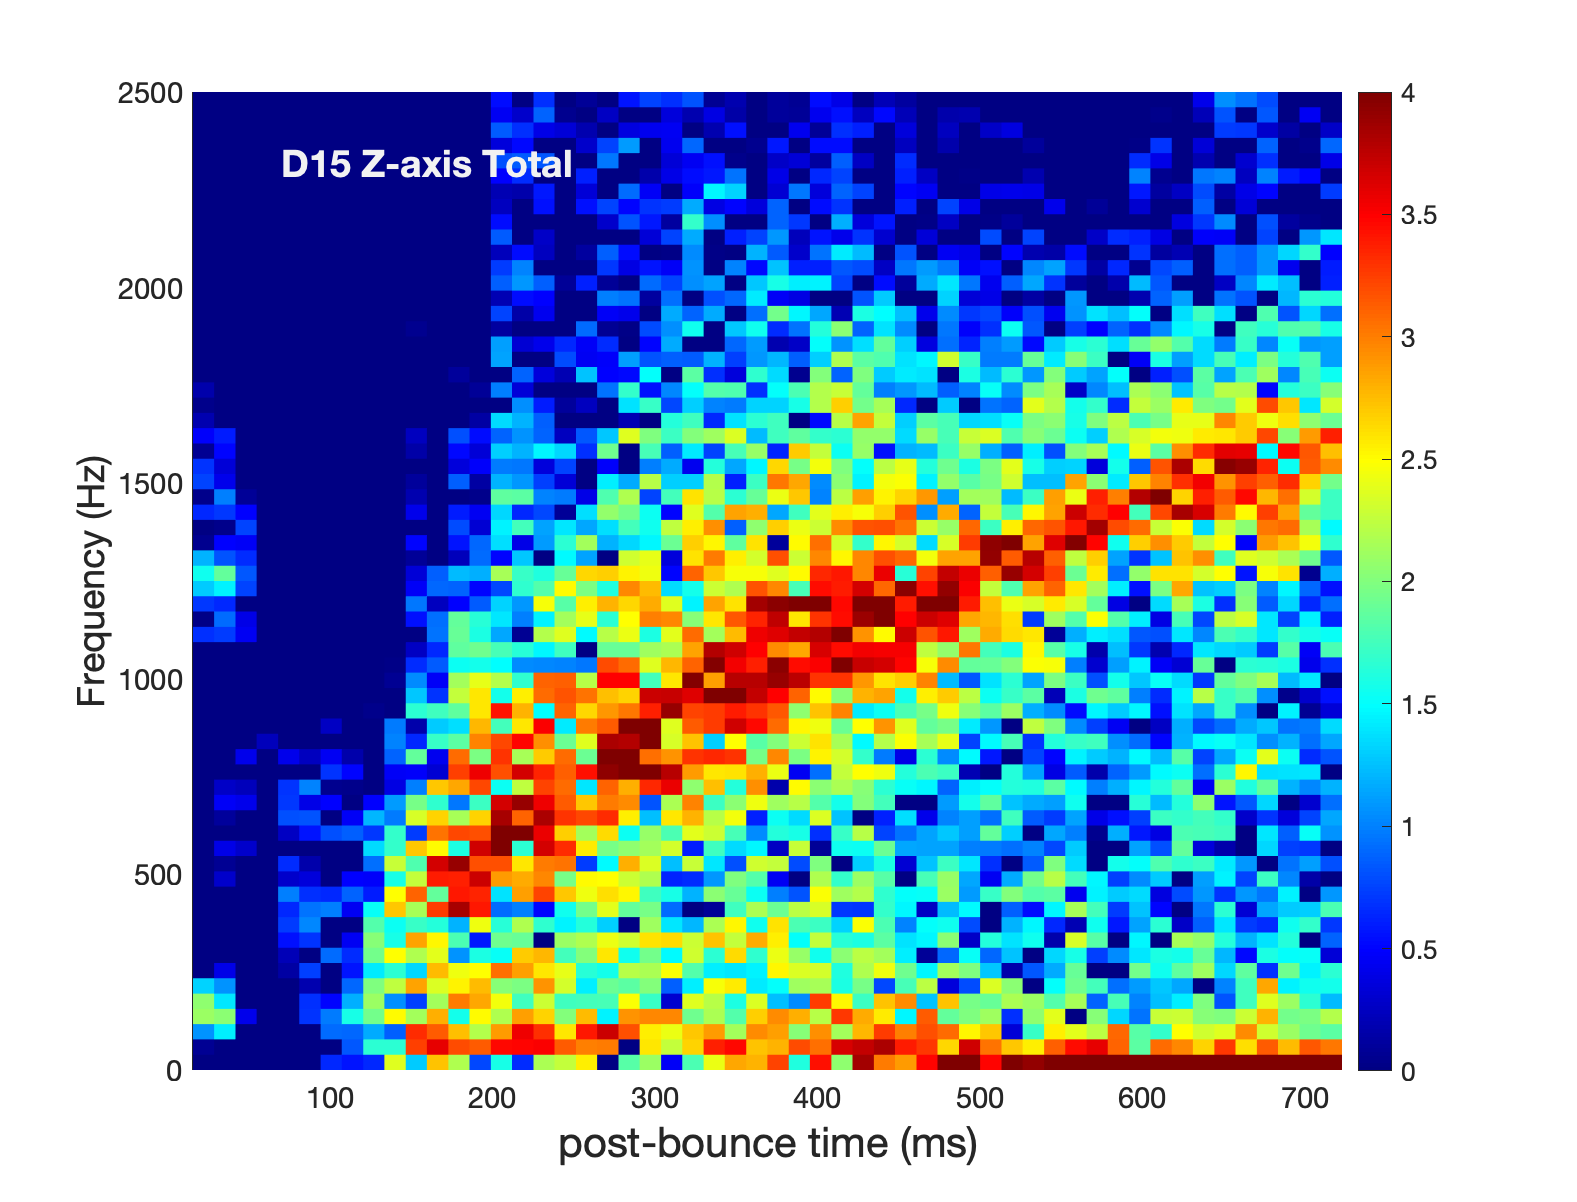
\includegraphics[width=0.25\textwidth]{Figures/D15_spectrogram_TOTAL.pdf}}
  \end{figure}

\end{frame}

\begin{frame}

  \begin{figure}
    \centering
    \subfloat{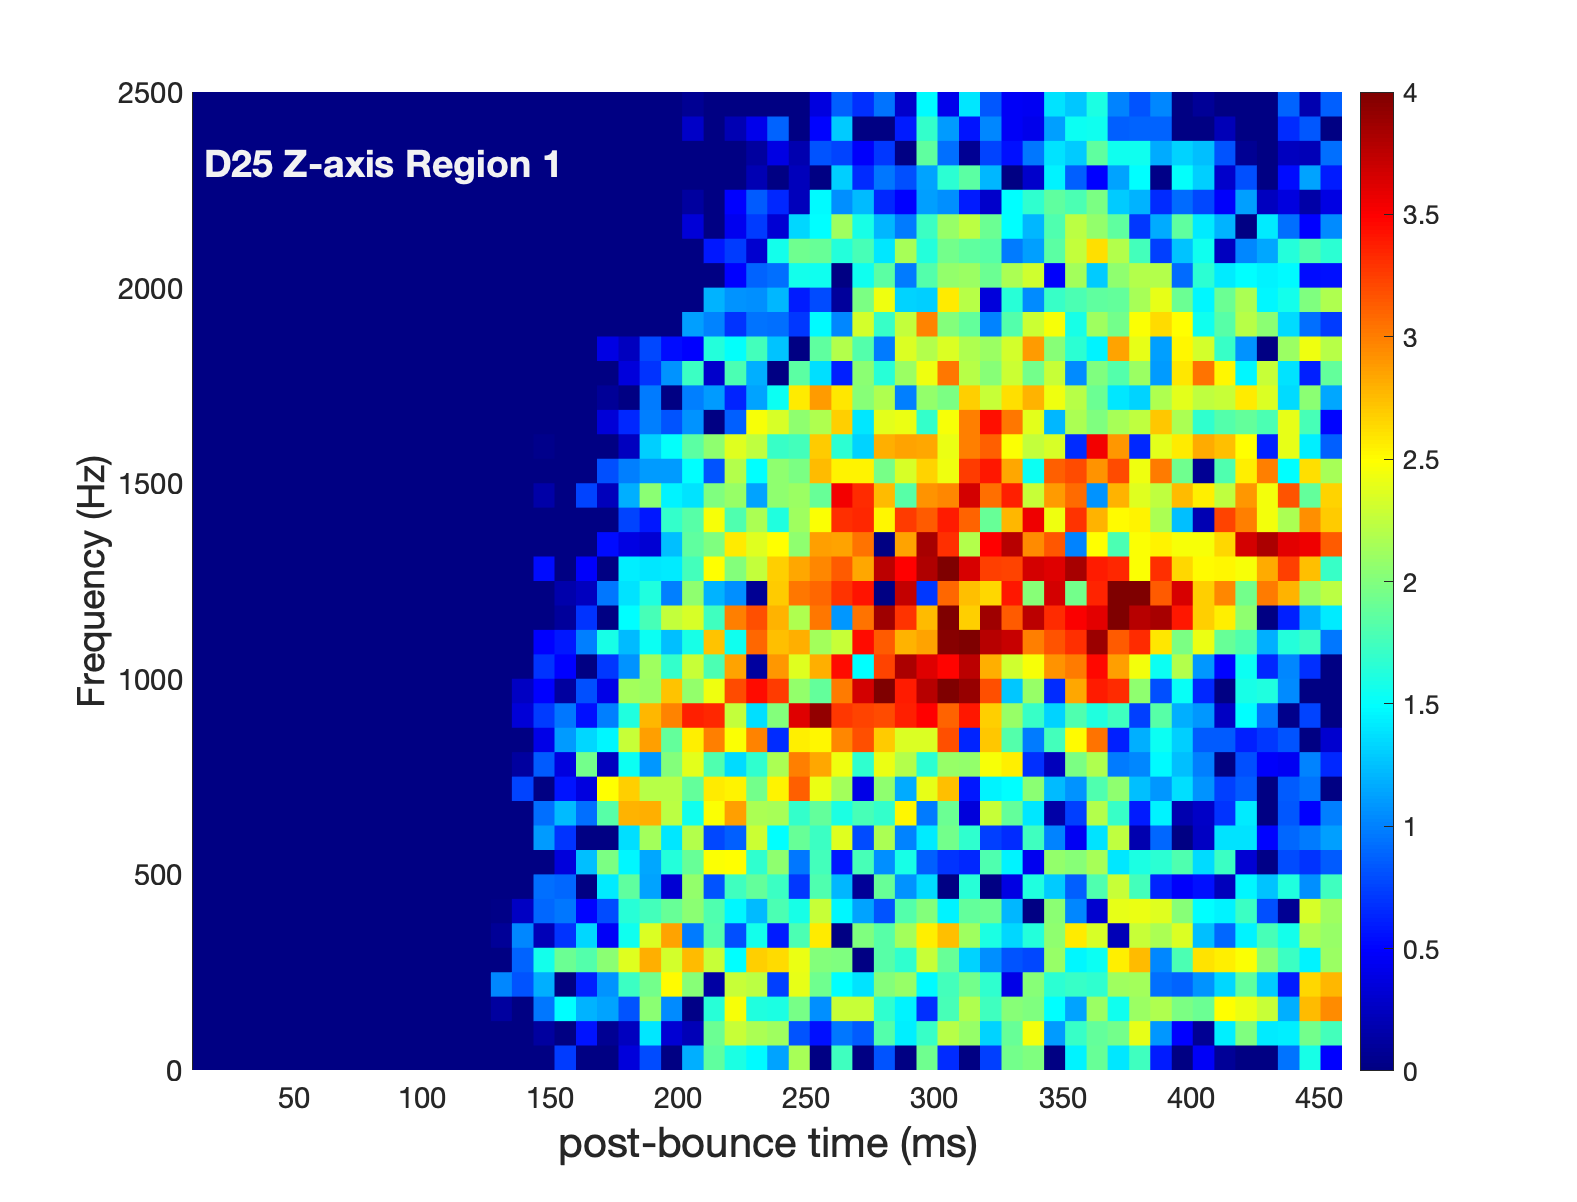
\includegraphics[width=0.25\textwidth]{Figures/D25_spectrogram_region01.pdf}}
    \subfloat{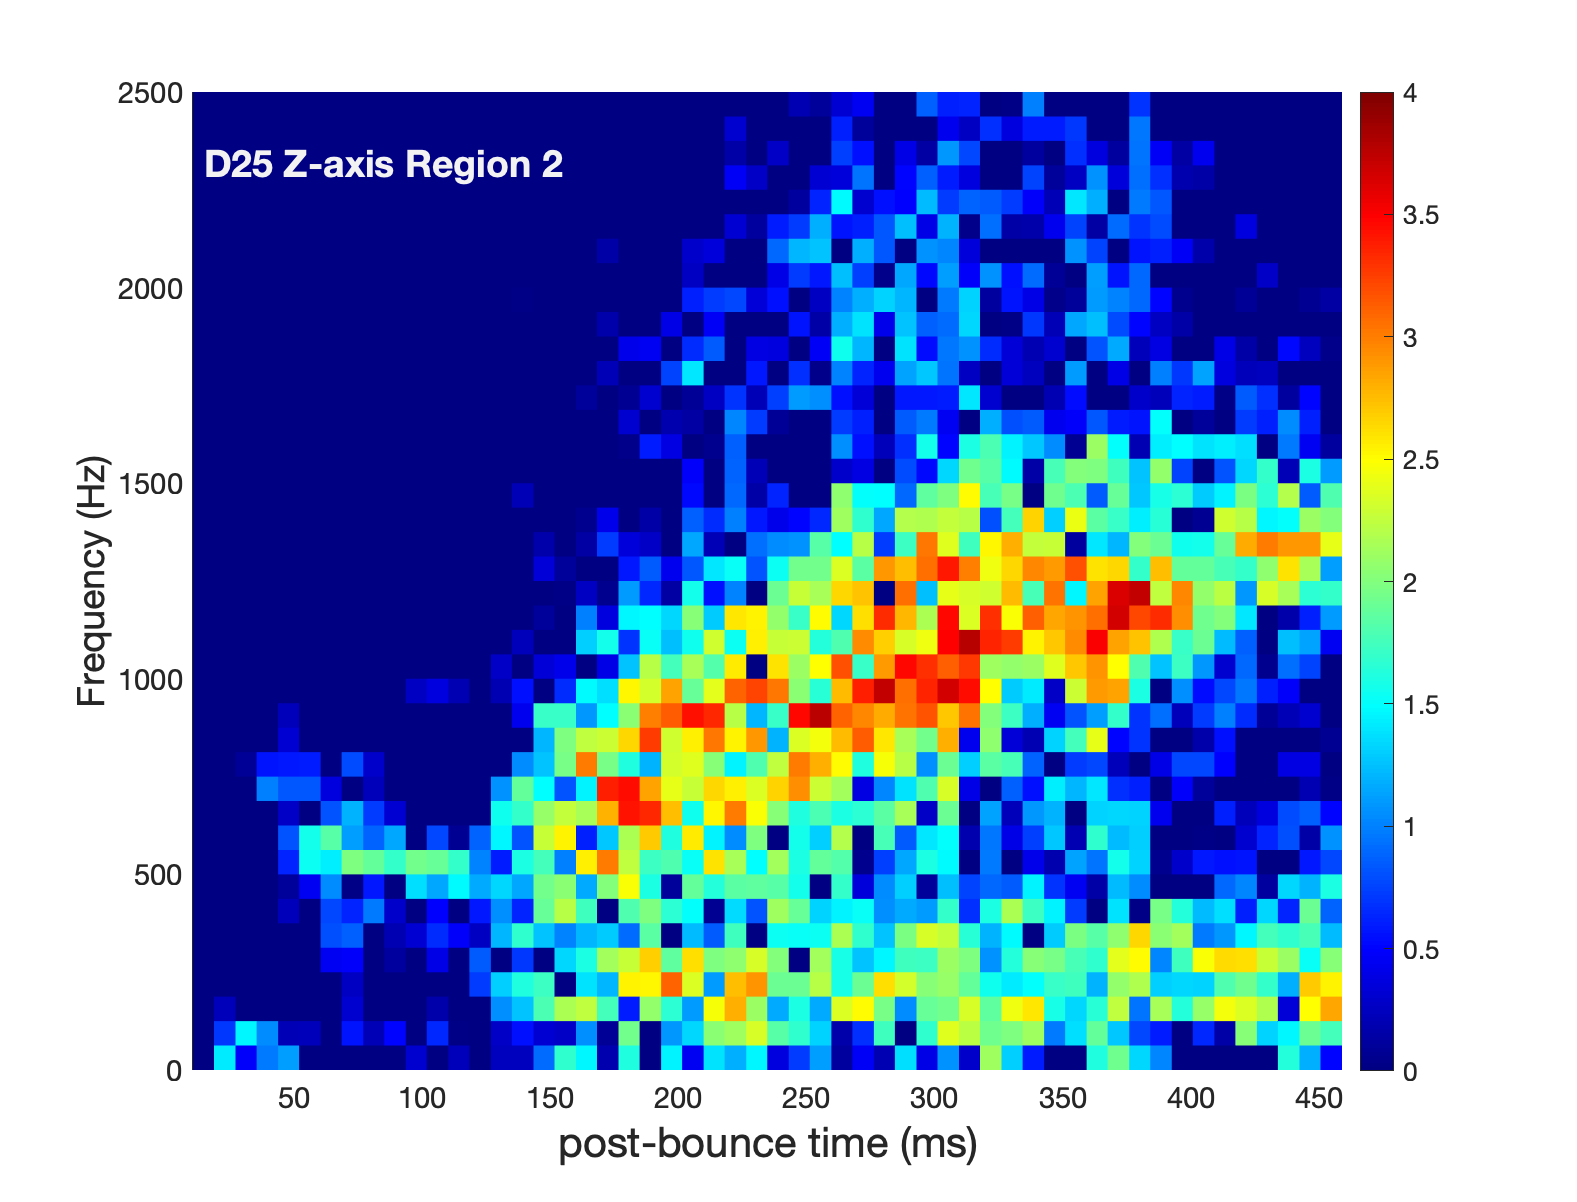
\includegraphics[width=0.25\textwidth]{Figures/D25_spectrogram_region02.pdf}}
    \subfloat{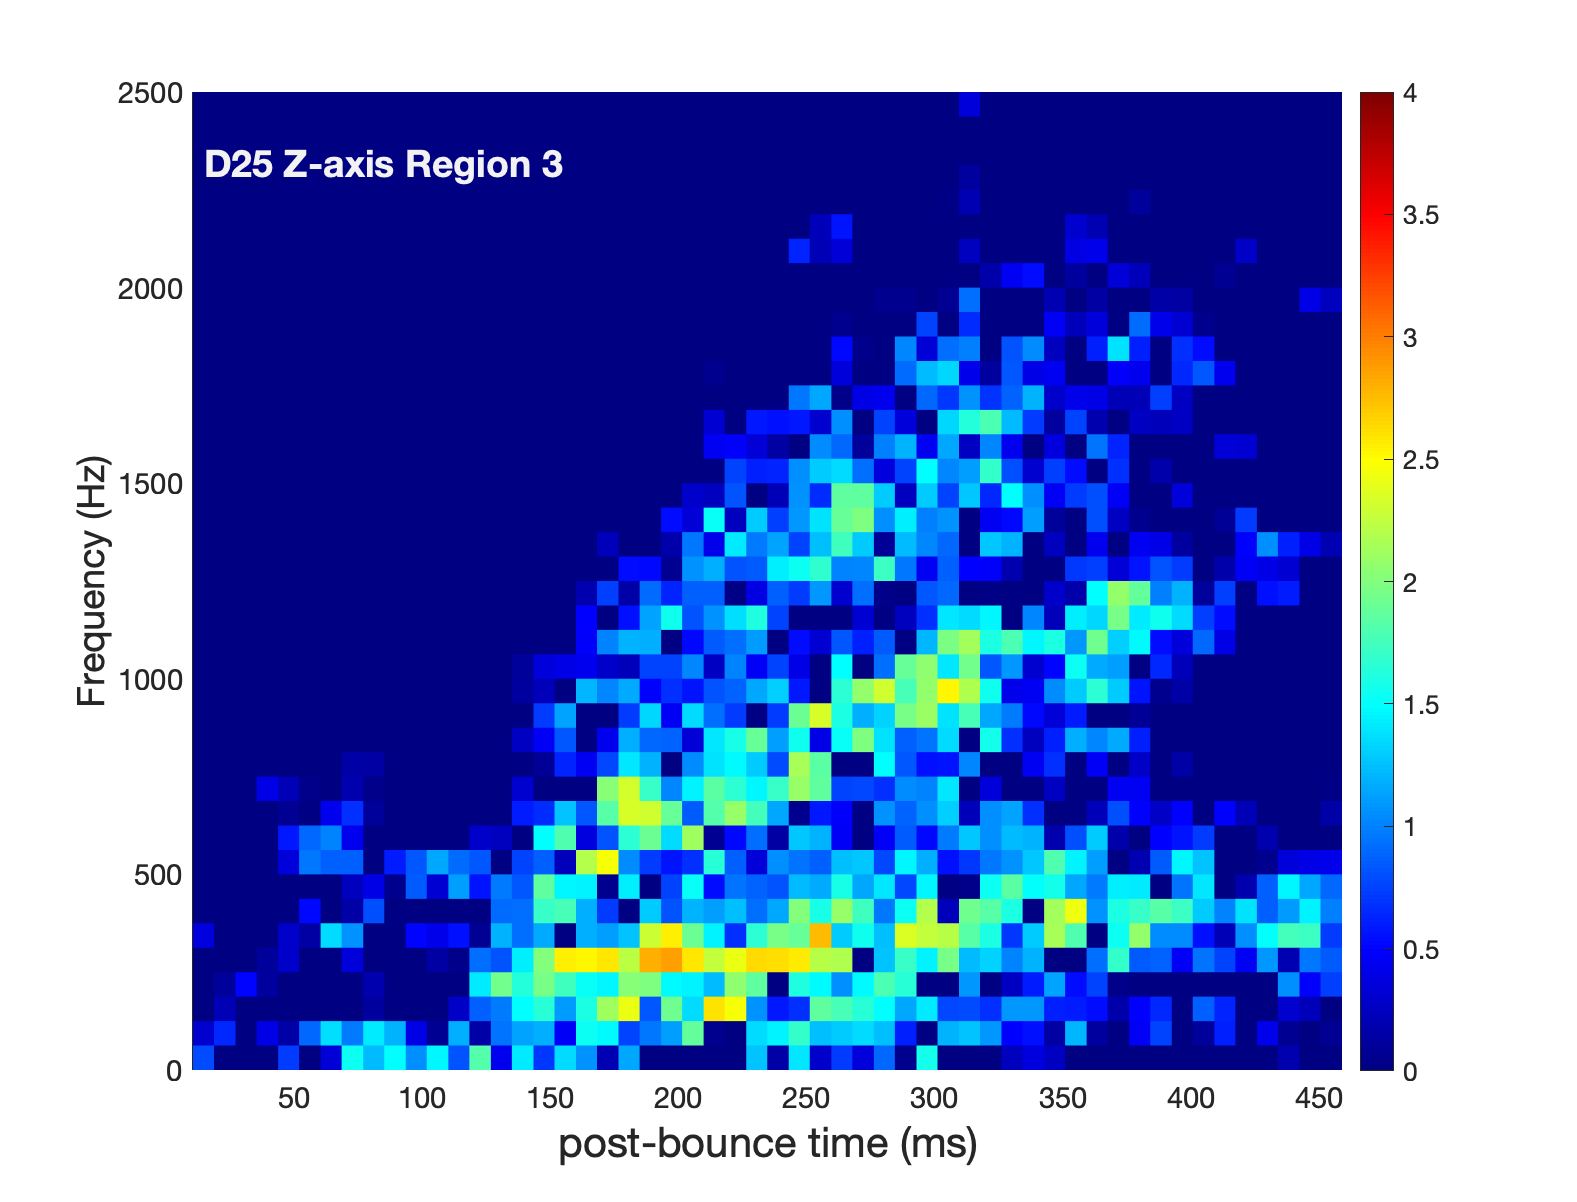
\includegraphics[width=0.25\textwidth]{Figures/D25_spectrogram_region03.pdf}}
  \end{figure}
  \vspace{-2em}
  \begin{figure}
    \centering
    \subfloat{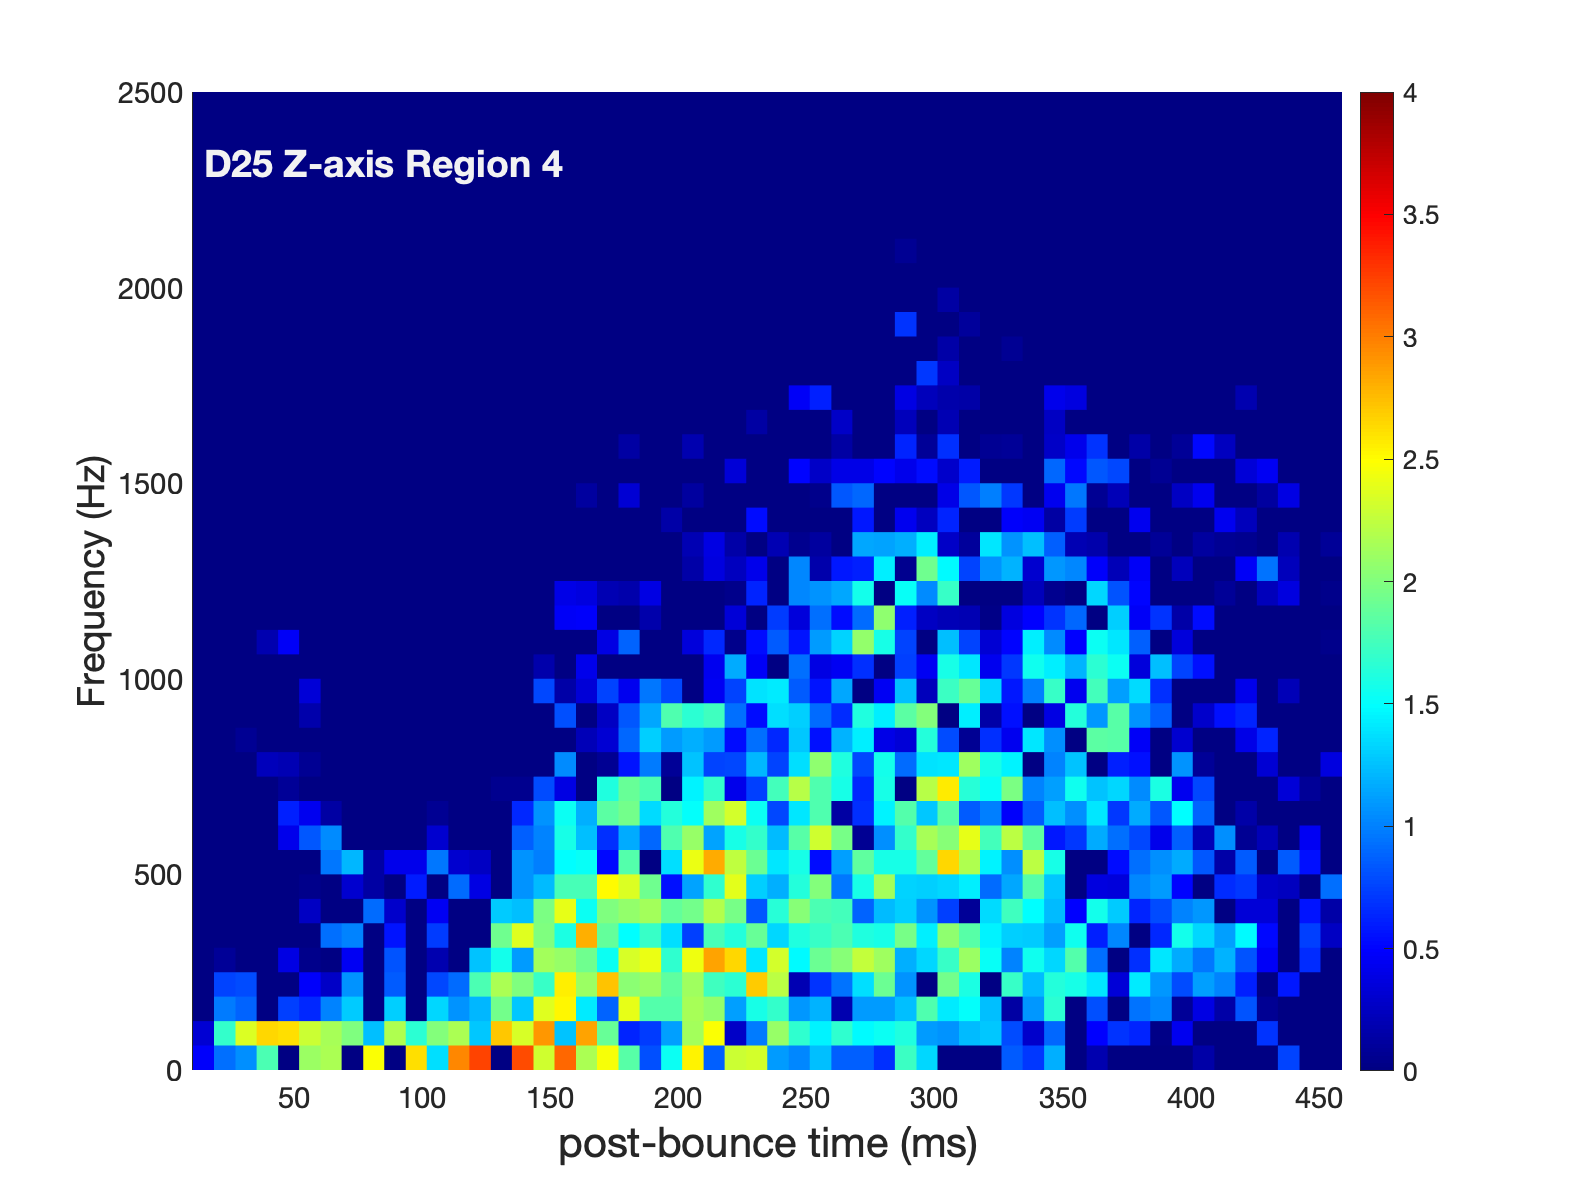
\includegraphics[width=0.25\textwidth]{Figures/D25_spectrogram_region04.pdf}}
    \subfloat{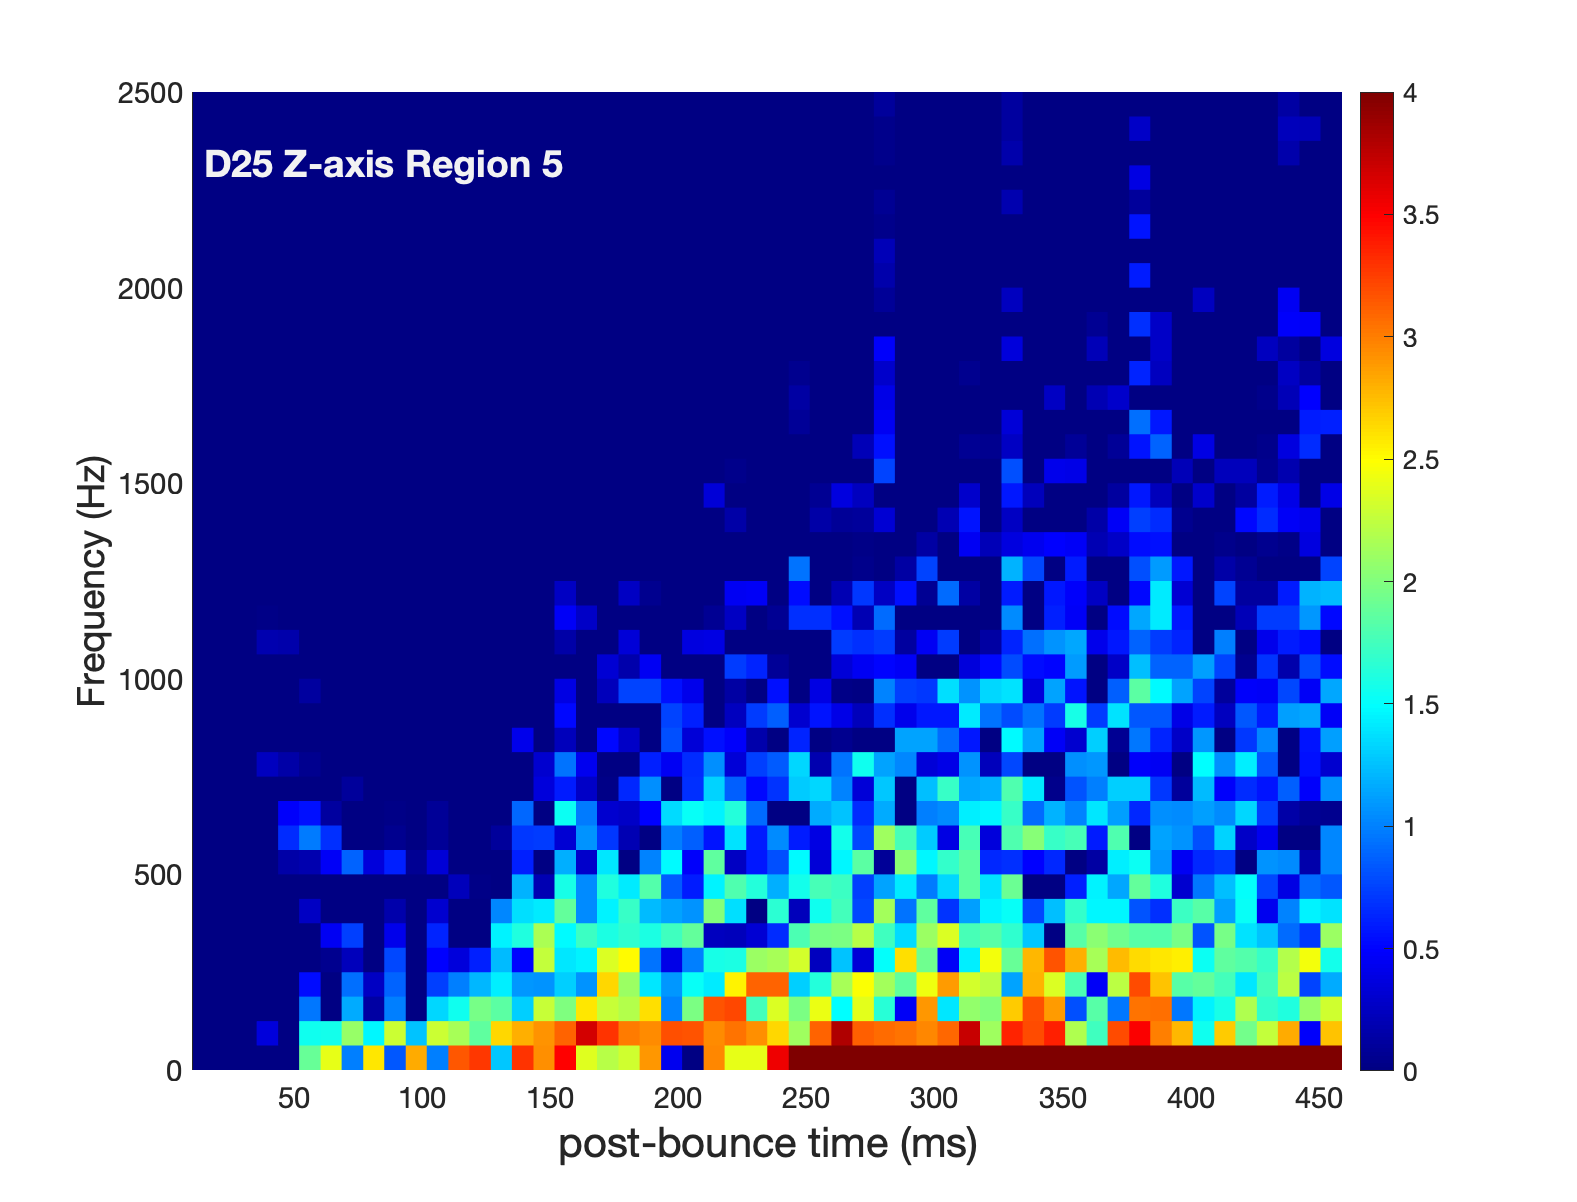
\includegraphics[width=0.25\textwidth]{Figures/D25_spectrogram_region05.pdf}}
    \subfloat{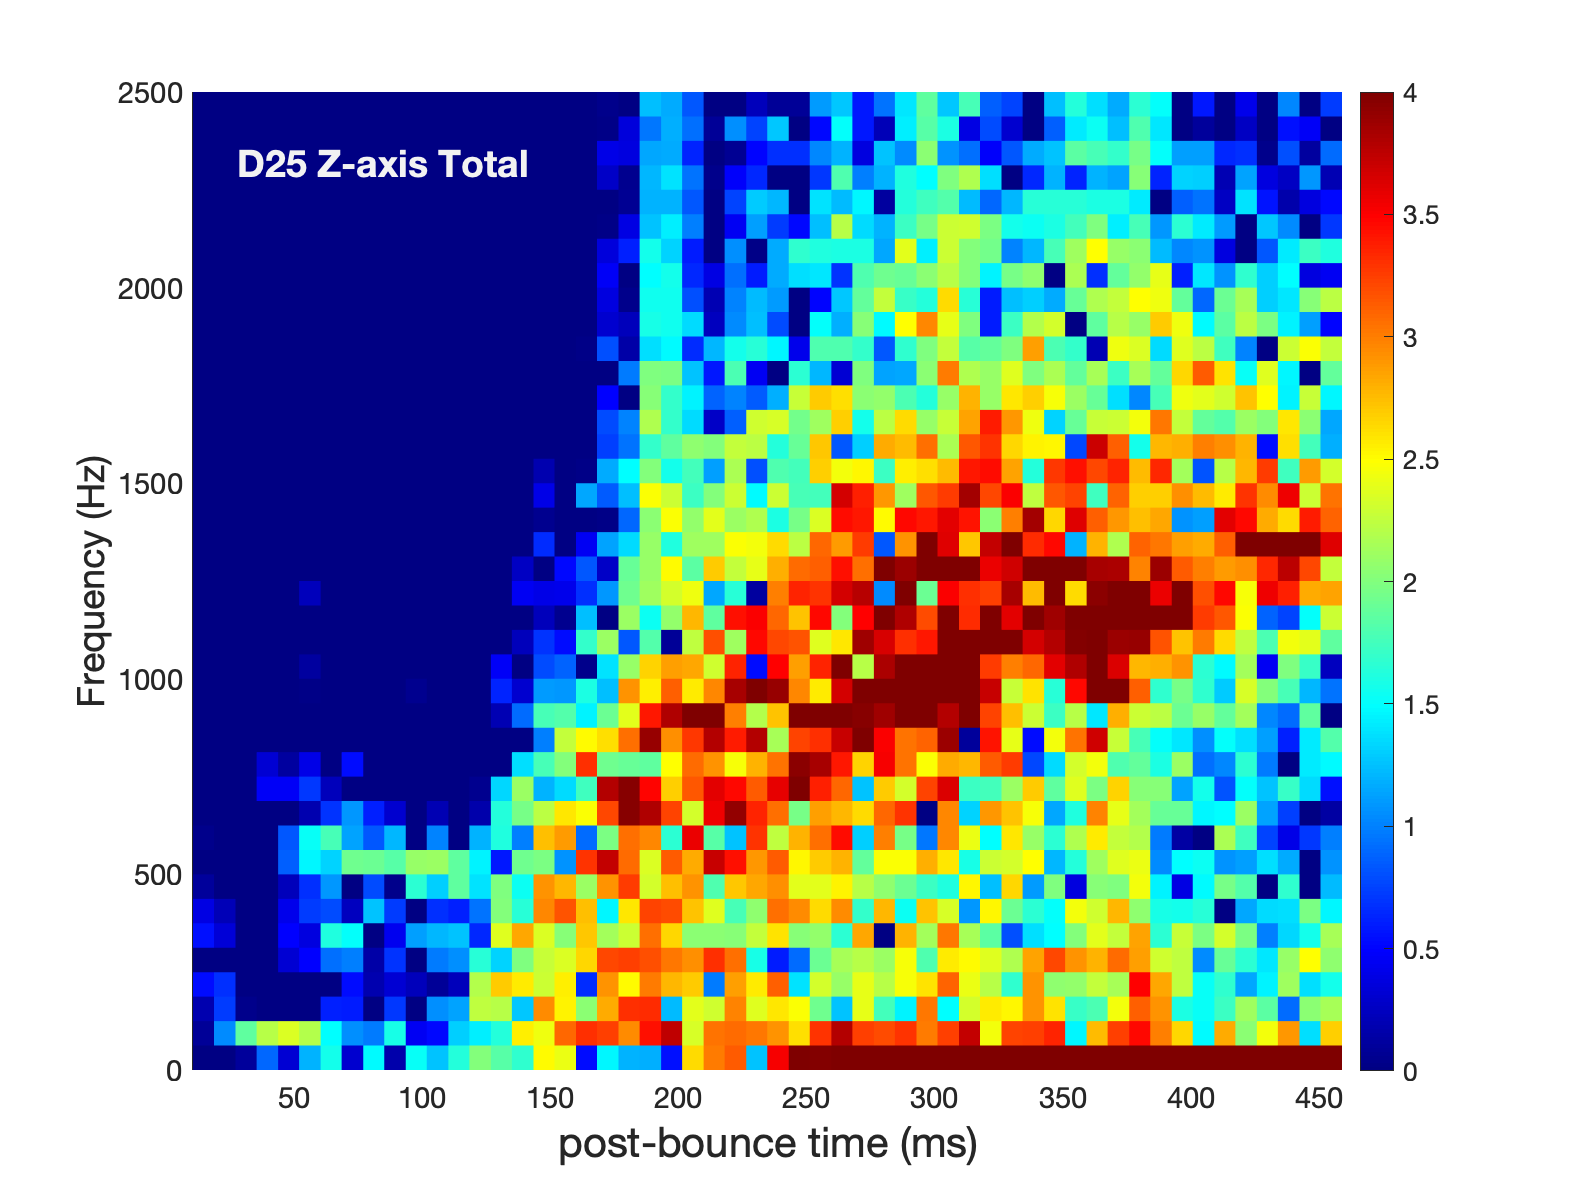
\includegraphics[width=0.25\textwidth]{Figures/D25_spectrogram_TOTAL.pdf}}
  \end{figure}

\end{frame}

\subsection{Peak Frequency Evolution}

\begin{frame}

  \begin{columns}[c]

    \column{.5\textwidth} % Left column and width
      \begin{equation*}
      f_{p}=\frac{1}{2\pi}\,\frac{G\,\mpns}{\rpns^{2}}\,\frac{1}{c_{s}}
      \,\sqrt{\Gamma-1}\,\left(1-\frac{G\,\mpns}{\rpns\,c^{2}}\right)^{3/2}
      \end{equation*}

    \column{.5\textwidth} % Left column and width
      \begin{figure}
        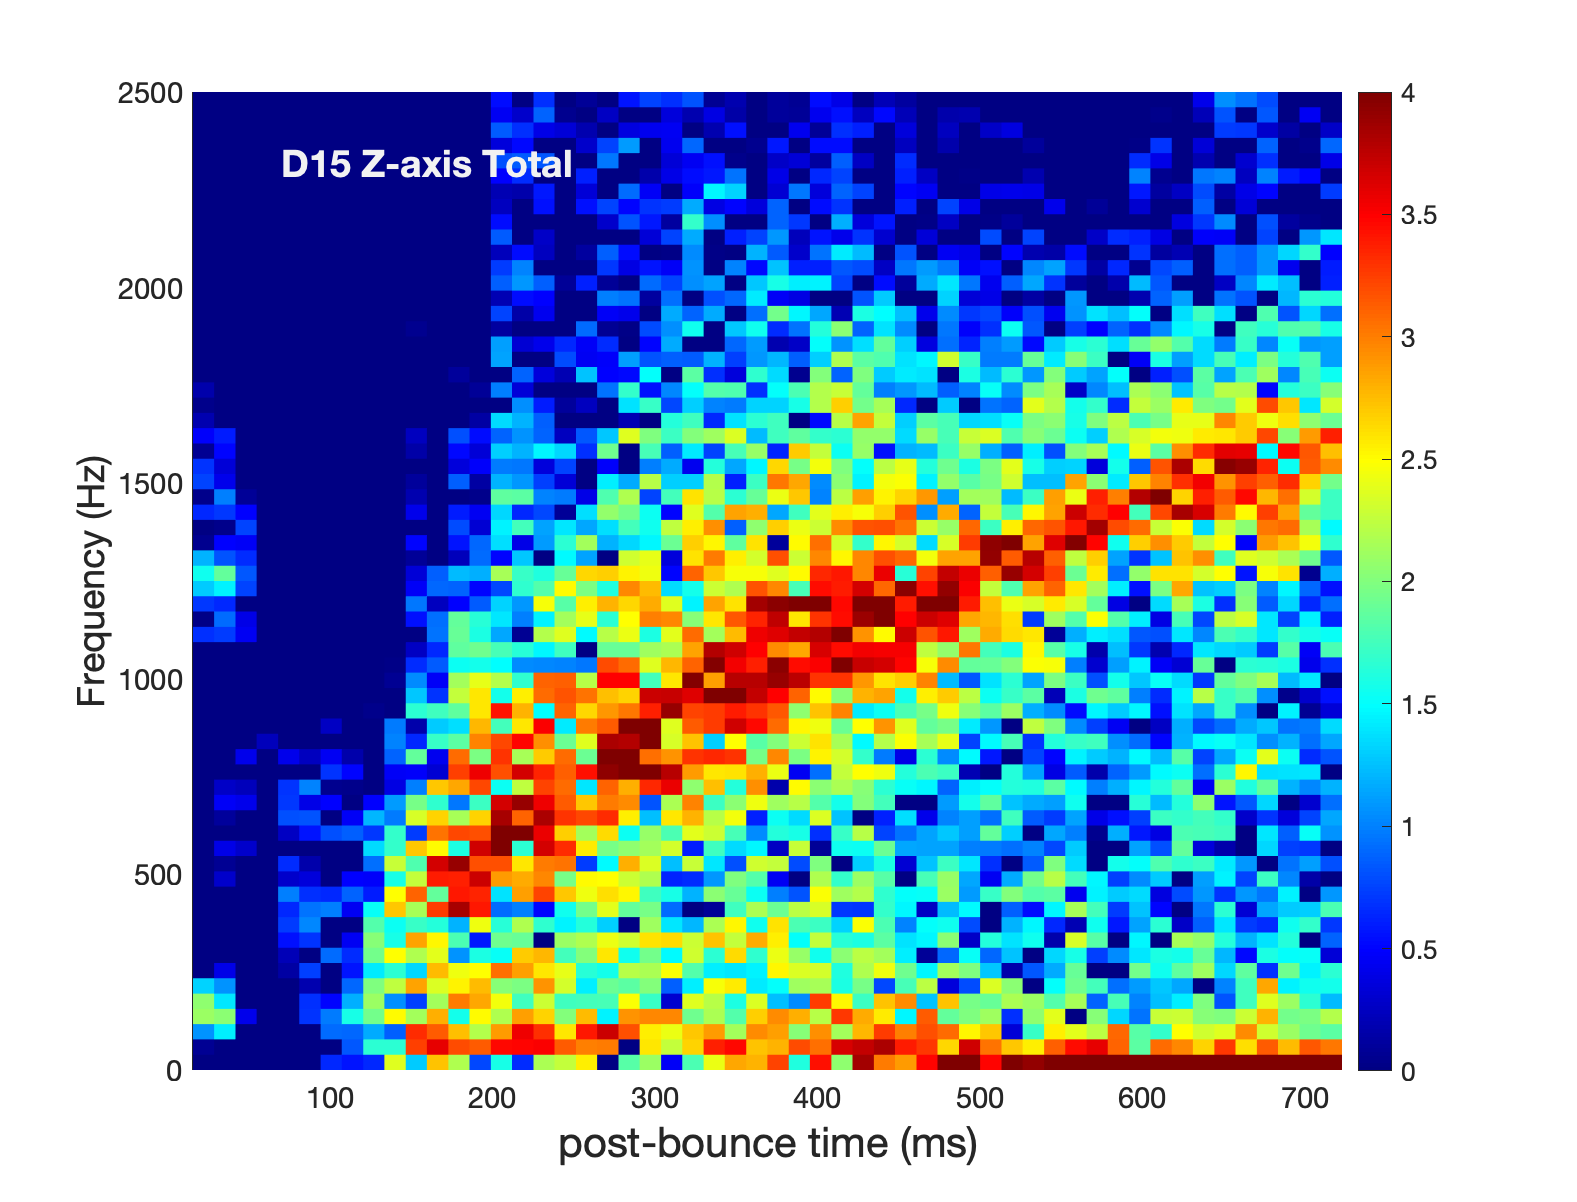
\includegraphics[width=1.0\textwidth]{Figures/D15_spectrogram_TOTAL.pdf}
      \end{figure}

  \end{columns}

\end{frame}

\begin{frame}

  \begin{columns}[c]

    \column{.33\textwidth} % Left column and width
      \begin{figure}
        \textbf{D9.6}
        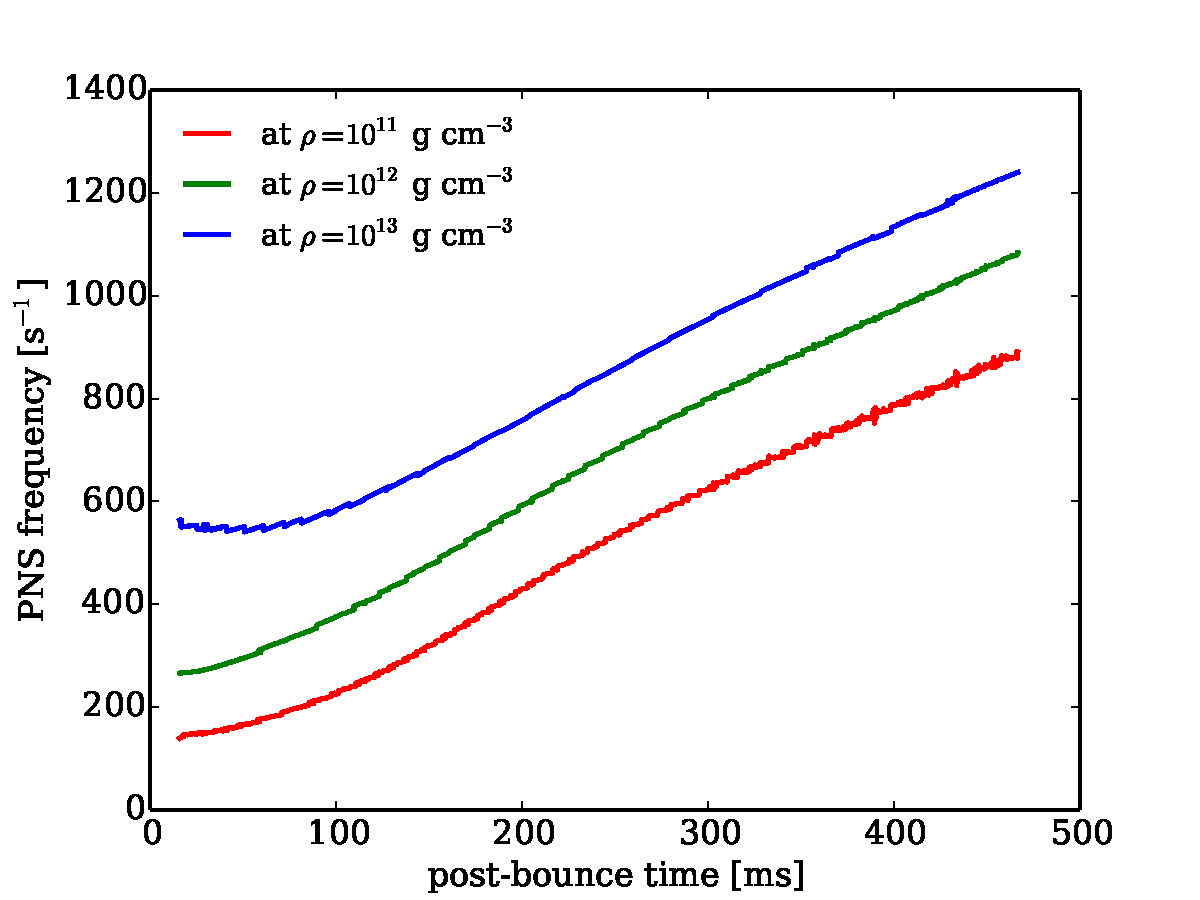
\includegraphics[width=1.0\textwidth]{Figures/D9.6_peakFrequency.pdf}
      \end{figure}

    \column{.33\textwidth} % Left column and width
      \begin{figure}
        \textbf{D15}
        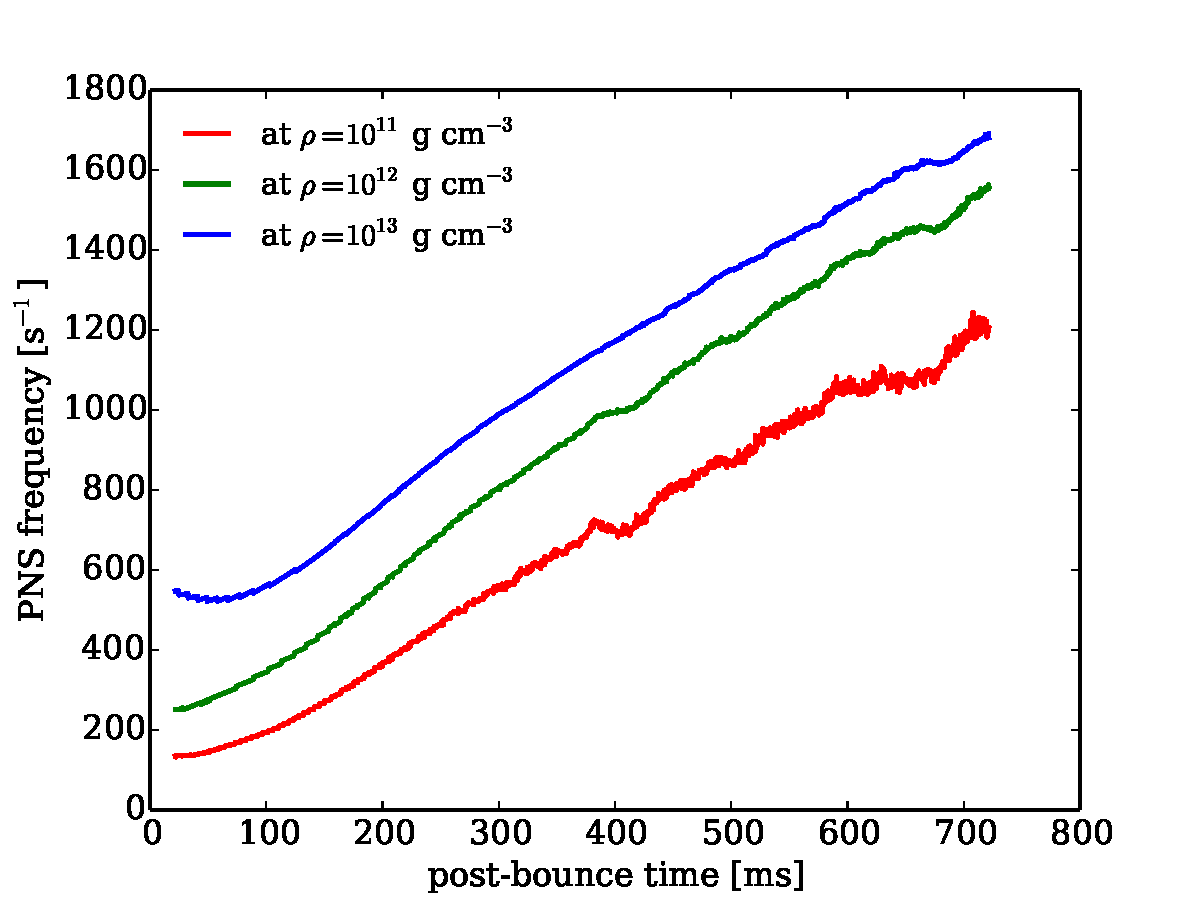
\includegraphics[width=1.0\textwidth]{Figures/D15_peakFrequency.pdf}
      \end{figure}

    \column{.33\textwidth} % Right column and width
      \begin{figure}
        \textbf{D25}
        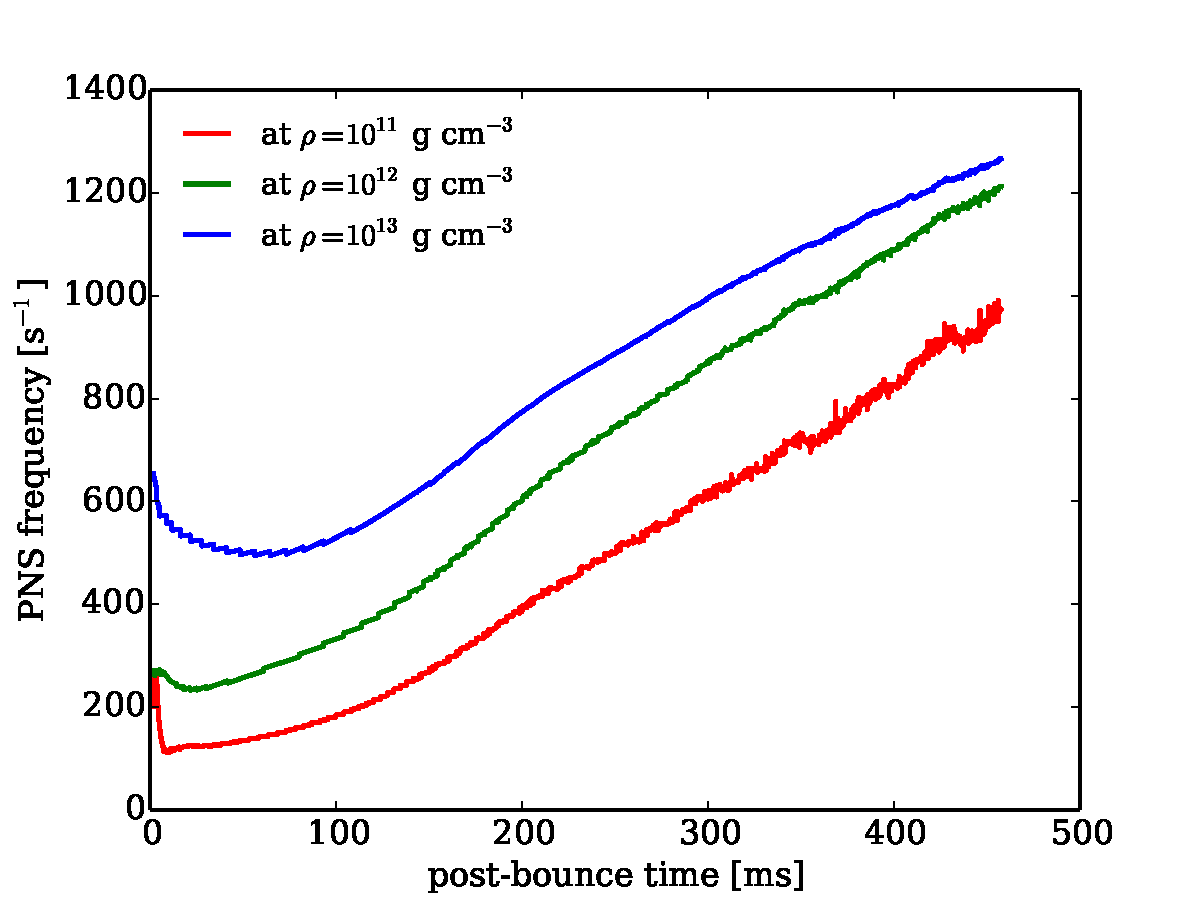
\includegraphics[width=1.0\textwidth]{Figures/D25_peakFrequency.pdf}
      \end{figure}

  \end{columns}

\end{frame}

\subsection{Luminosity and Energy}

\begin{frame}

  \begin{figure}
    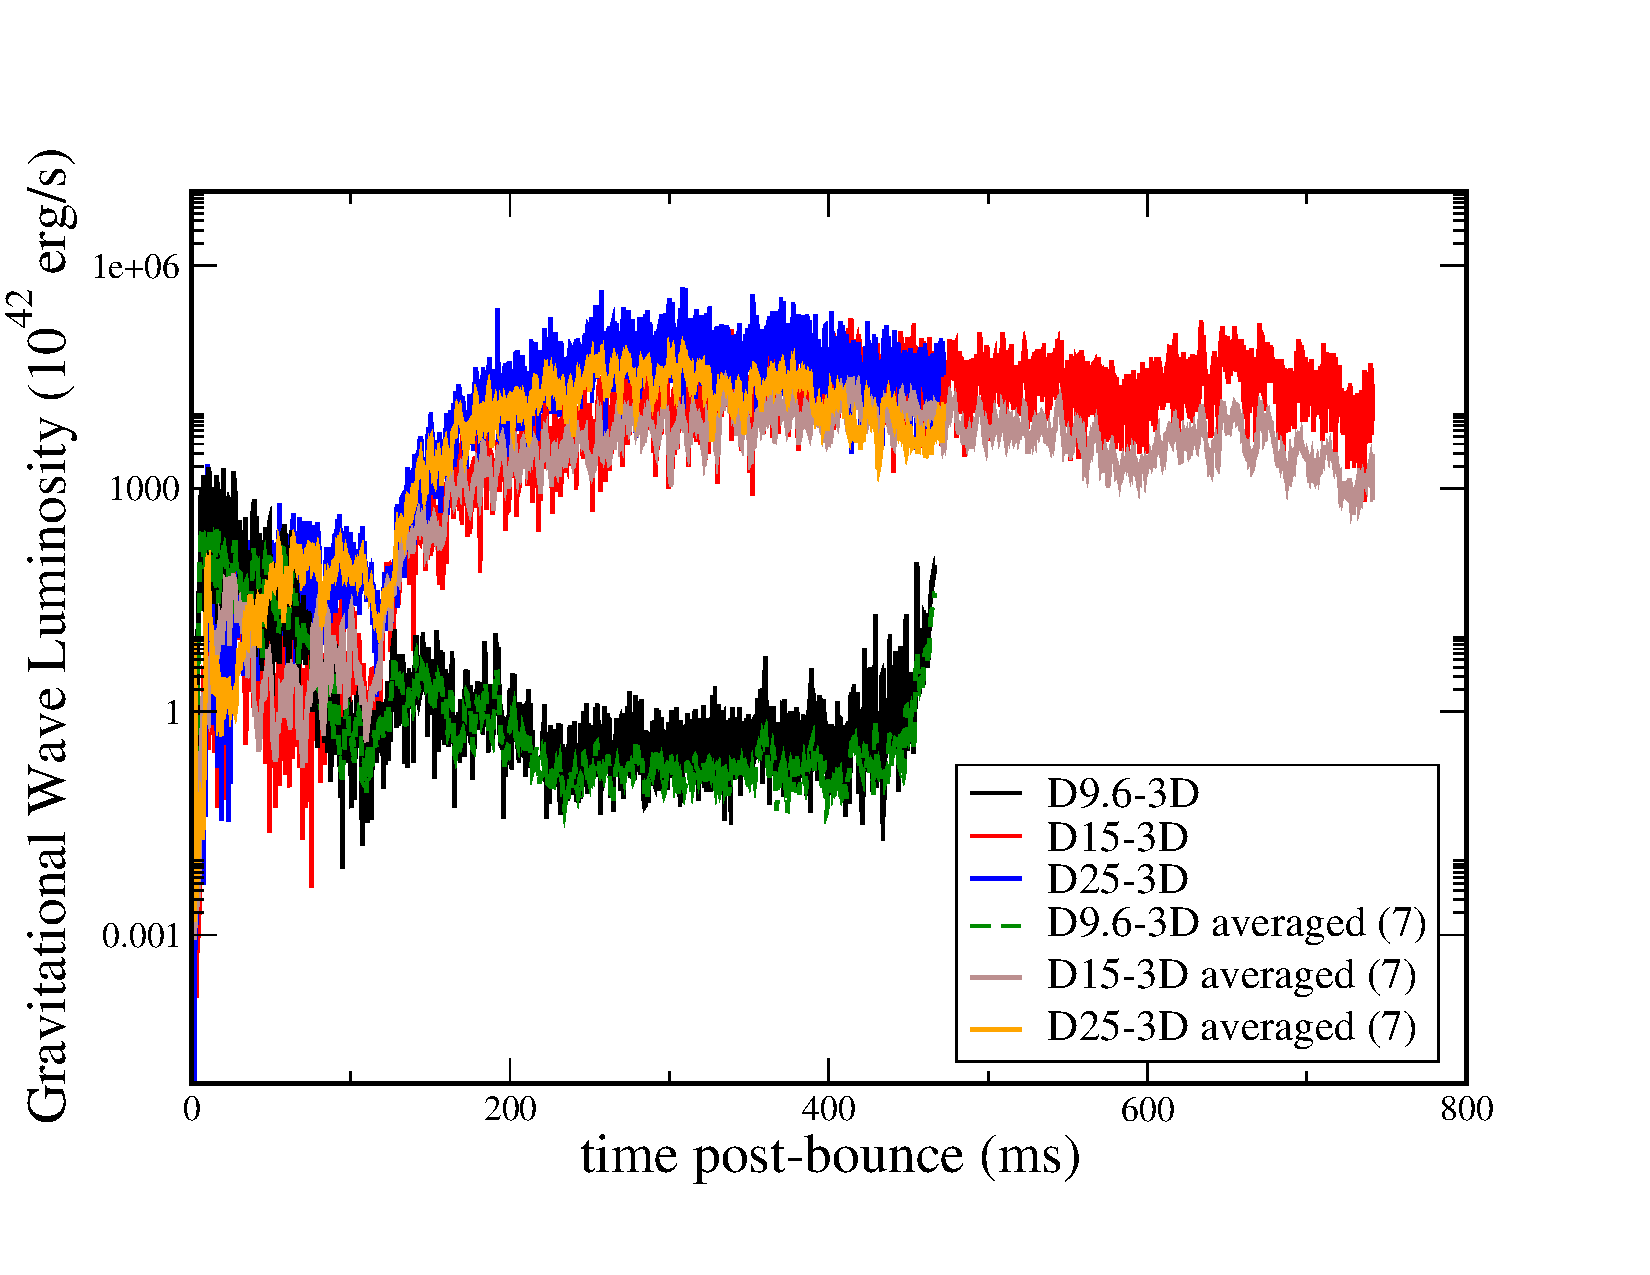
\includegraphics[width=0.7\textwidth]{Figures/Luminosity.pdf}
  \end{figure}

\end{frame}

\begin{frame}

  \begin{columns}[c]

    \column{0.5\textwidth}
    \begin{figure}
      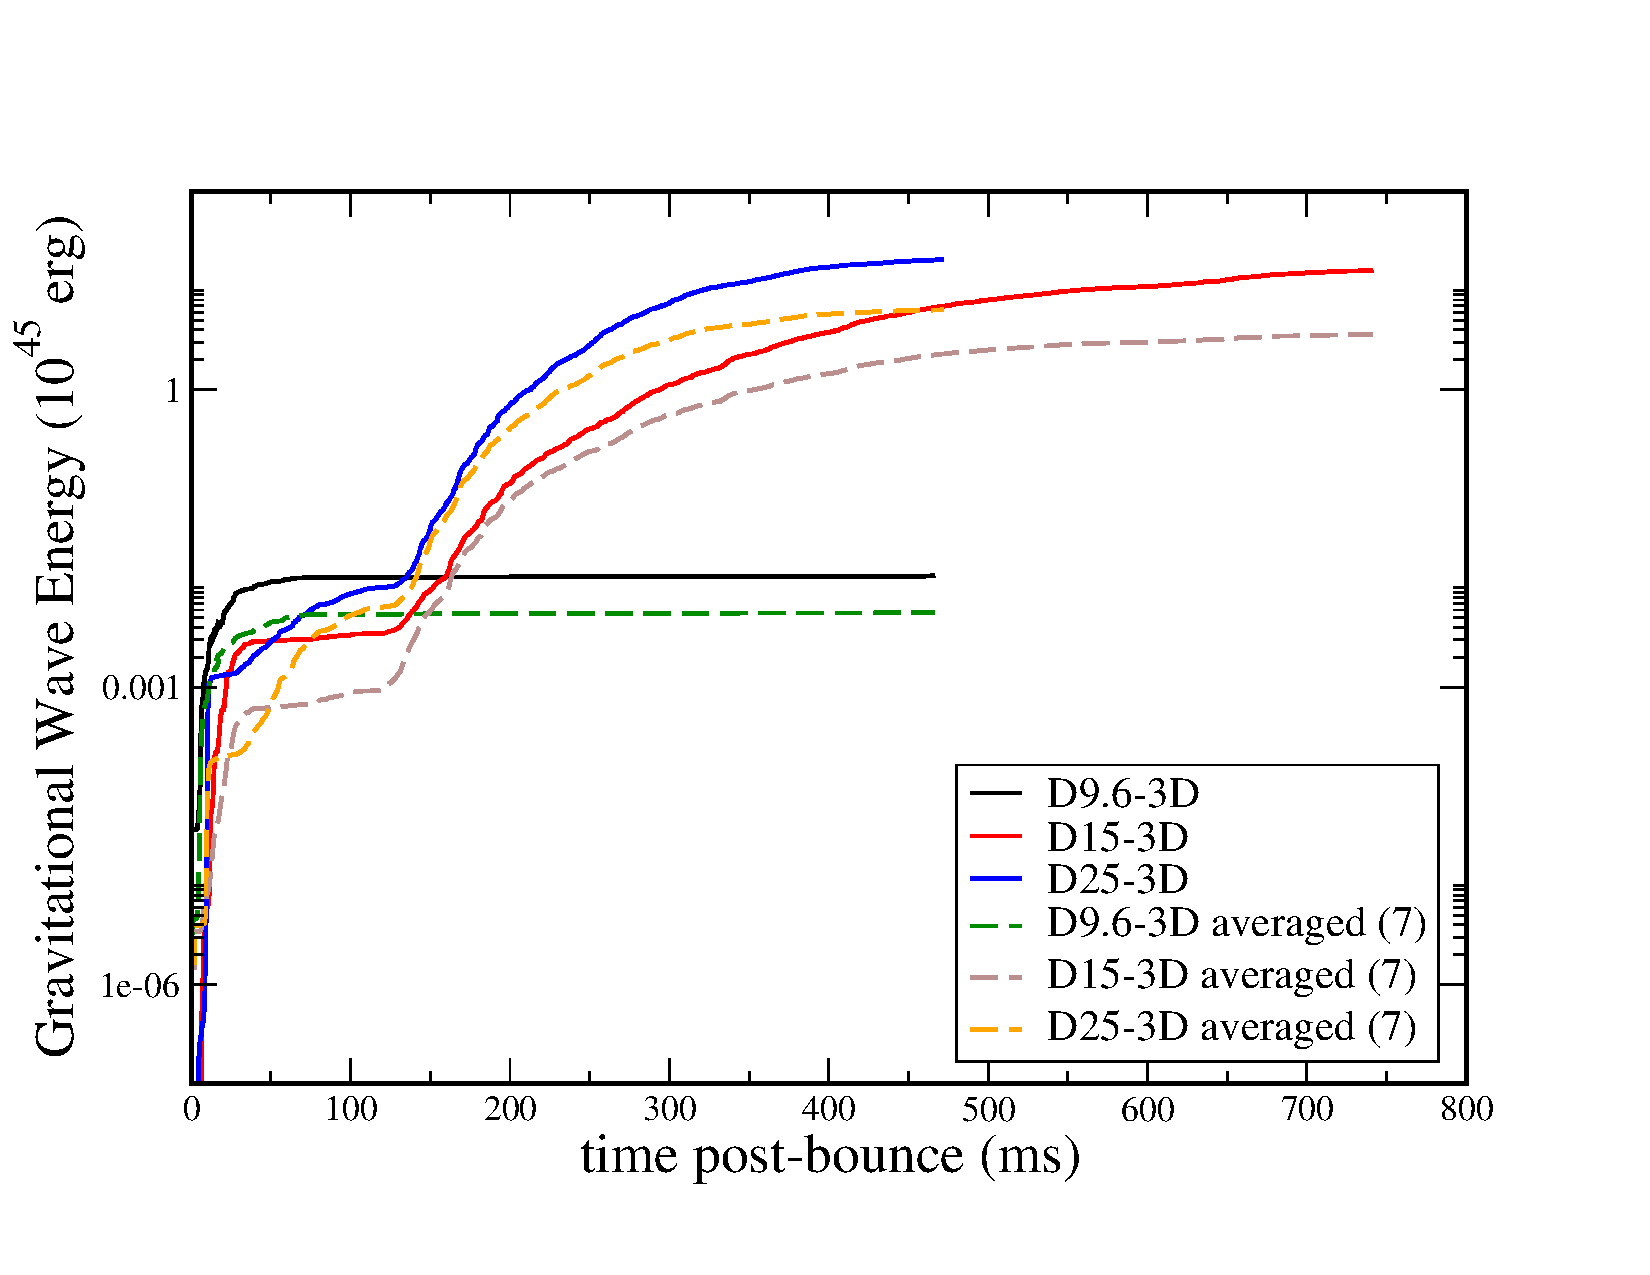
\includegraphics[width=1.0\textwidth]{Figures/Energy_all.pdf}
    \end{figure}

    \column{0.5\textwidth}
    \begin{figure}
      \includegraphics[width=1.0\textwidth]{Figures/Energy_D15.pdf}
    \end{figure}

  \end{columns}

\end{frame}

\subsection{Spectra}

\begin{frame}

  \centerline{\textbf{Recall: assumed SN distance of 10 kpc}}

  \begin{columns}[c]

    \column{0.33\textwidth}
    \begin{figure}
      \includegraphics[width=1.0\textwidth]{Figures/D9.6_hchar.pdf}
    \end{figure}

    \column{0.33\textwidth}
    \begin{figure}
      \includegraphics[width=1.0\textwidth]{Figures/D15_hchar.pdf}
    \end{figure}

    \column{0.33\textwidth}
    \begin{figure}
      \includegraphics[width=1.0\textwidth]{Figures/D25_hchar.pdf}
    \end{figure}

  \end{columns}

\end{frame}

\subsection{SASI}

\begin{frame}

  \begin{columns}[c]

    \column{0.33\textwidth}
    \begin{figure}
      \textbf{D9.6}
      \includegraphics[width=1.0\textwidth]{Figures/D9.6_com.pdf}
    \end{figure}

    \column{0.33\textwidth}
    \begin{figure}
      \textbf{D15}
      \includegraphics[width=1.0\textwidth]{Figures/D15_com.pdf}
    \end{figure}

    \column{0.33\textwidth}
    \begin{figure}
      \textbf{D25}
      \includegraphics[width=1.0\textwidth]{Figures/D25_com.pdf}
    \end{figure}

  \end{columns}

\end{frame}

\begin{frame}

  \begin{columns}[c]

    \column{0.33\textwidth}
    \begin{figure}
      $t<75\,\ms$
      \includegraphics[width=1.0\textwidth]{Figures/D9.6_PreE.pdf}
    \end{figure}

    \column{0.33\textwidth}
    \begin{figure}
      $t<300\,\ms$
      \includegraphics[width=1.0\textwidth]{Figures/D15_PreE.pdf}
    \end{figure}

    \column{0.33\textwidth}
    \begin{figure}
      $t<180\,\ms$
      \includegraphics[width=1.0\textwidth]{Figures/D25_PreE.pdf}
    \end{figure}

  \end{columns}

\end{frame}

\begin{frame}

  \begin{columns}[c]

    \column{0.33\textwidth}
    \begin{figure}
      $t>75\,\ms$
      \includegraphics[width=1.0\textwidth]{Figures/D9.6_PostE.pdf}
    \end{figure}

    \column{0.33\textwidth}
    \begin{figure}
      $t>300\,\ms$
      \includegraphics[width=1.0\textwidth]{Figures/D15_PostE.pdf}
    \end{figure}

    \column{0.33\textwidth}
    \begin{figure}
      $t>180\,\ms$
      \includegraphics[width=1.0\textwidth]{Figures/D25_PostE.pdf}
    \end{figure}

  \end{columns}

\end{frame}

\subsection{Numerical Method Comparison}

\begin{frame}

  In the weak-field limit,
  \begin{equation*}
    I_{2m}:=\frac{16\,\sqrt{3}\,\pi}{15}\int\rho\,Y^{*}_{2m}\,r^{2}\,dV,
  \end{equation*}
  with
  \begin{equation*}
  dV:=r^{2}\,\sin\theta\,dr\,d\theta\,d\varphi.
  \end{equation*}
  For numerical reasons,
  \begin{equation*}
  A_{2m}:=\frac{G}{c^{4}}\,\frac{d^{2}I_{2m}}{dt^{2}}=\frac{dN_{2m}}{dt},
  \end{equation*}
  where
  \begin{equation*}
  N_{2m}:=\frac{G}{c^{4}}\,\frac{dI_{2m}}{dt}.
  \end{equation*}

\end{frame}

\begin{frame}

  \begin{align*}
  N_{2m}&=\frac{16\,\sqrt{3}\,\pi\,G}{15\,c^{4}}
  \int_{0}^{2\pi}d\varphi'\,\int_{0}^{\pi}d\theta'\int_{a}^{b}dr'\,r'^{3}\\
  &\times\left[2\,\rho\,v^{r}\,Y^{*}_{2m}\,\sin\theta'
  +\rho\,v^{\theta}\,\sin\theta'\,\pd{}{\theta'}Y^{*}_{2m}
  +\rho\,v^{\varphi}\,\pd{}{\varphi'}\,Y^{*}_{2m}\right]\\
  &-\frac{16\,\sqrt{3}\,\pi\,G}{15\,c^{4}}
  \int_{0}^{2\pi}d\varphi'\,\int_{0}^{\pi}d\theta'
  Y^{*}_{2m}\,\sin\theta'\left(r_{b}^{4}\,\rho_{b}\,v_{b}^{r}
  -r_{a}^{4}\,\rho_{a}\,v_{a}^{r}\right)\\
  &=:\bar{N}_{2m}+\Delta N_{2m}.
  \end{align*}

\end{frame}

\begin{frame}

  \centerline{\textbf{D15}}

  \begin{columns}[c]

    \column{0.5\textwidth}
    \begin{figure}
      \includegraphics[width=1.0\textwidth]{Figures/D15_N2mvsN2mbar.pdf}
    \end{figure}

    \column{0.5\textwidth}
    \begin{figure}
      \includegraphics[width=1.0\textwidth]{Figures/D15_N2mvsI2m.pdf}
    \end{figure}

  \end{columns}

\end{frame}

\begin{frame}

  \centerline{\textbf{D25}}

  \begin{columns}[c]

    \column{0.5\textwidth}
    \begin{figure}
      \includegraphics[width=1.0\textwidth]{Figures/D25_N2mvsN2mbar.pdf}
    \end{figure}

    \column{0.5\textwidth}
    \begin{figure}
      \includegraphics[width=1.0\textwidth]{Figures/D25_N2mvsI2m.pdf}
    \end{figure}

  \end{columns}

\end{frame}

\begin{frame}

  \centerline{\textbf{D9.6}}

  \begin{columns}[c]

    \column{0.5\textwidth}
    \begin{figure}
      \includegraphics[width=1.0\textwidth]{Figures/D9.6_N2mvsN2mbar.pdf}
    \end{figure}

    \column{0.5\textwidth}
    \begin{figure}
      \includegraphics[width=1.0\textwidth]{Figures/D9.6_N2mvsI2m.pdf}
    \end{figure}

  \end{columns}

\end{frame}


\subsection{Resolution}

\begin{frame}

  \begin{figure}
    \includegraphics[width=0.7\textwidth]{Figures/C15_D15_rh_Zaxis.pdf}
  \end{figure}

\end{frame}

%-------------------------------------------------------------------------------
\section{Bibliography}
%-------------------------------------------------------------------------------

\begin{frame}

  [1] Mezzacappa, A. et al.
      arXiv:2208.10643 (2022).\newline

  [2] Mezzacappa, A.
      \textit{Annual Review of Nuclear and Particle Science}
      \textbf{55}:467-515 (2005).\newline

  [3] Mezzacappa, A. et al.
      \textit{Phys. Rev. D}
      \textbf{102},023027 (2020).\newline

  [4] M{\"u}ller, B. \textit{Living Rev Comput Astrophys}
      \textbf{6},3 (2020).

\end{frame}

%-------------------------------------------------------------------------------
\section{Conclusions}
%-------------------------------------------------------------------------------

\begin{frame}

  \begin{itemize}
    \item Progenitor structure imprinted on GW signal
    \item D9.6 qualitatively different from D15 and D25
    \item Strains observable with LVK
    \item Definition of PNS surface important
    \item Resolution important
  \end{itemize}

\end{frame}

%-------------------------------------------------------------------------------
\section{Secret Tracks}
%-------------------------------------------------------------------------------

\subsection{Strains}

\begin{frame}

  \begin{align*}
    h^{\textsc{tt}}_{ij}
    &:=\frac{G}{c^{4}}\,\frac{1}{r}\sum\limits_{m=-2}^{+2}
    \frac{d^{2}I_{2m}}{dt^{2}}\left(t-\frac{r}{c}\right)\,f^{2m}_{ij}\\
    h_{+}&:=\frac{h_{\theta\theta}^{\textsc{tt}}}{r^{2}},\\
    h_{\times}
    &:=\frac{h_{\theta\varphi}^{\textsc{tt}}}{r^{2}\,\sin^{2}\theta}
  \end{align*}

\end{frame}

\begin{frame}

  \begin{align*}
    f^{2m}_{ij}&:=\alpha\,r^{2}
    \begin{pmatrix}
    0&0&0\\
    0&W_{2m}&X_{2m}\\
    0&X_{2m}&-W_{2m}\,\sin^{2}\theta
    \end{pmatrix}\\
    X_{2m}&:=2\,\pd{}{\varphi}\left(\pd{}{\theta}-\cot\theta\right)
    Y_{2m}\left(\theta,\varphi\right)\\
    W_{2m}&:=\left(\pd{^{2}}{\theta^{2}}
    -\cot\theta\,\pd{}{\theta}
    -\frac{1}{\sin^{2}\theta}\,\pd{^{2}}{\varphi^{2}}\right)\,
    Y_{2m}\left(\theta,\varphi\right)\\
    \alpha\textrm{ defined such that}&
    \int_{\mathbb{S}^{2}}d\Omega
    \left(f_{lm}\right)_{ab}\left(f^{*}_{l'm'}\right)_{cd}\,
    \gamma^{ac}\,\gamma^{bd}=r^{4}\,\delta_{ll'}\,\delta_{mm'},\\
    &\textrm{where }a,b,c,d\in\left\{\theta,\varphi\right\},\textrm{ and}\\
    \gamma_{ab}&=\begin{pmatrix}1&0\\0&\sin^{2}\theta\end{pmatrix}
  \end{align*}

\end{frame}

\subsection{Luminosity and Energy}

\begin{frame}

  The total luminosity emitted in gravitational waves is given by
  \begin{equation*}
    \frac{dE}{dt}=\frac{c^{3}}{G}\,\frac{1}{32\pi}
    \sum\limits_{m=-2}^{+2}\left<\left|\frac{dA_{2m}}{dt}\right|^{2}\right>,
  \end{equation*}
  where $\left<\right>$ means ``average over several wave cycles".
  The total energy emitted in gravitaional waves is then
  \begin{align*}
    E&=\int_{-\infty}^{+\infty}\frac{dE}{dt}\,dt
    =\frac{c^{3}}{32\pi G}\sum\limits_{m=-2}^{+2}
    \int_{-\infty}^{+\infty}\left|\dot{A}_{2m}\right|^{2}dt\\
    &\stackrel{\mathrm{FT}}{=}
    \frac{c^{3}}{32\pi G}\sum\limits_{m=-2}^{+2}\int_{-\infty}^{+\infty}
    \left|\tilde{\dot{A}}_{2m}\left(2\pi\,f\right)\right|^{2}df\\
    &=\frac{c^{3}}{16\pi G}\sum\limits_{m=-2}^{+2}\int_{0}^{+\infty}
    \left|\tilde{\dot{A}}_{2m}\left(2\pi\,f\right)\right|^{2}df.
  \end{align*}

\end{frame}

\subsection{Spectra}

\begin{frame}

  \begin{equation*}
    \frac{dE}{df}=\frac{c^{3}}{16\pi G}\left(2\pi\,f\right)^{2}
    \sum\limits_{m=-2}^{+2}\left|\tilde{A}_{2m}\right|^{2}
  \end{equation*}

\end{frame}

\begin{frame}

  Using short-time Fourier transform techniques,
  \begin{equation*}
    \tilde{A}_{2m}\left(\tau,f\right)
    =\int_{-\infty}^{+\infty}A_{2m}\left(t\right)\,H\left(t-\tau\right)
    e^{-i\,2\pi\,f\,t}\,dt,
  \end{equation*}
  where $H$ is the Hann window function and they set $\tau=15\,\ms$.

\end{frame}

\subsection{Characteristic Frequency}

\begin{frame}

  Under assumptions of redshift $z=0$,
  \begin{equation*}
  h_{\mathrm{char}}\left(f\right)
  =\sqrt{\frac{2G}{\pi^{2}c^{3}D^{2}}\,\frac{dE}{df}}.
  \end{equation*}
  They set $D=10\,\kpc$.

\end{frame}

\end{document}
